\documentclass[15pt, aspectratio=169]{beamer}
\usepackage[backend=biber]{biblatex}

\usetheme[progressbar=frametitle]{metropolis}
\usepackage{appendixnumberbeamer}

\usepackage{booktabs}
\usepackage[scale=3]{ccicons}

\usepackage{graphicx}

\usepackage{amsmath}

\usepackage{tikz}

\usepackage{pgfplots}
\usepgfplotslibrary{dateplot}

\usepackage[labelformat=empty]{caption}

%\usepackage[dvipsnames]{xcolor}
%\definecolor{Background}{HTML}{F0F0F0}
%\definecolor{Foreground}{HTML}{23373B}




\usepackage{xspace}
\newcommand{\themename}{\textbf{\textsc{metropolis}}\xspace}
\usepackage[utf8]{inputenc}

%\setbeamercovered{transparent}
%\setbeamertemplate{navigation symbols}{}
%\setbeamertemplate{caption}{}
\setbeamertemplate{frame footer}[frame number]

\makeatletter
\setlength{\metropolis@titleseparator@linewidth}{2pt}
\setlength{\metropolis@progressonsectionpage@linewidth}{2pt}
\setlength{\metropolis@progressinheadfoot@linewidth}{2pt}
\makeatother

\addbibresource{/home/giorgio/Bibliography/bibliography.bib}


\title{Preparazione di polvere di biopolimeri}
\subtitle{Stampa 3D tramite Selective Laser Sintering}
% \date{\today}
\date{}
\author{Giorgio De Trane}
\institute{Politecnico di Torino}
\titlegraphic{\hfill
\includegraphics[height=1.5cm]{Pictures/Vector/PDF/polito_logo.pdf}}

\begin{document}

\maketitle

\begin{frame}{Contenuti}
  \setbeamertemplate{section in toc}[sections numbered]
  \tableofcontents[hideallsubsections]
\end{frame}


\section{Introduzione}
  \subsection{Obiettivi}

  \begin{frame}{Obiettivi}

    \onslide+<1-4>{
      \begin{center}
        \alert<1>{Qual è lo scopo di questa tesi?}
      \end{center}
    
    }

    
    \begin{itemize}
      \item <2->\textbf{Preparazione} di polvere di biopolimeri
      \item <3->\textbf{Stampa 3D} di biopolimeri
    \end{itemize}

  %  \onslide<4->{
  %    \begin{center}
  %      La stampa 3D è un processo con molteplici applicazioni
  %    \end{center}
  %  }
  \end{frame}

  \begin{frame}
    \frametitle{Biopolimeri}
    \begin{center}
        Perchè utilizzare i \textbf{biopolimeri}?
    \end{center}
    \begin{figure}[h]
      \centering
      
\includegraphics[width=0.3\textwidth]{Pictures/Vector/PDF/hand_bio.pdf}
      
    \end{figure}

  \end{frame}

  \begin{frame}
    \frametitle{Perchè biopolimeri?}
    \begin{itemize}
      \item <1->\textbf{Biodegradabili}
      \item <2->\textbf{Biocompatibili}
      \item <3->\textbf{Riciclabili}
      \item <4->\textbf{Sostenibili}
    \end{itemize}

    \only<1>{Possono essere smaltiti e degradati attraverso processi enzimatici, esattamente come sono stati prodotti}
    \only<2>{Sono compatibili con i tessuti umani e ampiamente utilizzati in campo biomedico}
    \only<3>{Possono essere rilavorati e riutilizzati per altri scopi}
    \only<4>{Dalla produzione allo smaltimento, in linea con le guidelines dell'UE per la sostenibilità}
    

  \end{frame}

  \begin{frame}
    \frametitle{Stampa 3D}

    
    \begin{center}
      Perchè utilizzare la \textbf{stampa 3D}?
    \end{center}
    \begin{figure}[h]
    \centering
    
\includegraphics[width=0.3\textwidth]{Pictures/Vector/PDF/3d_printing.pdf}

    \end{figure}


  \end{frame}

  \begin{frame}
    \frametitle{Perchè stampa 3D?}
    \begin{itemize}
      \item <1->\textbf{Libertà e flessibilità di design}
      \item <2->\textbf{Geometrie complesse}
      \item <3->\textbf{Minimo spreco di materiale}
      %\item <4->\textbf{Sostenibili}
    \end{itemize}
    \only<1>{Ci si può svincolare dai workflow restrittivi del CAD e della produzione tradizionale}
    \only<2>{Si possono realizzare geometrie complesse e irraggiungibili con altri metodi di produzione}
    \only<3>{Si minimizza l'utilizzo di materiale, riducendo potenzialmente i costi e l'impatto ambientale}
    %\only<4>{Dalla produzione allo smaltimento, in linea con le guidelines dell'UE per la sostenibilità}
    
  \end{frame}
    
  
  
  \subsection{Ricerca}

  \begin{frame}{Ricerca}
    \onslide<1>{
      \begin{center}
        \alert{Cosa dice la letteratura?}
      \end{center}
    }
    \begin{itemize}
      \item <2-> Stato dell'arte dei \textbf{polimeri} nella \textbf{stampa 3D}
      \item <3->  \textbf{Biopolimeri} nella \textbf{stampa 3D}
      \item <4->  Produzione di \textbf{polvere} per \textbf{Selective Laser Sintering}
    \end{itemize}

    \only<2>{Ampiamente utilizzati, ma principalmente polimeri di origine petrolchimica}
    \only<3>{Utilizzo in crescita, ma principalmente in Fused Deposition Modeling}
    \only<4>{Precipitazione chimica o macinatura meccanica criogenica}

    \onslide<5>{\alert<5>{Pochissimi} risultati in letteratura!}

  \end{frame}

  \begin{frame}
    \frametitle{Selective Laser Sintering}

    \onslide*<1>{
      \begin{center}
        \alert<1>{Cosa è il Selective Laser Sintering?}
      \end{center}
      }
  
    \onslide*<2->{L'\textbf{SLS} 
    è una tecnologia di produzione additiva che impiega un laser per \alert<3>{sinterizzare} delle particelle 
    di polvere polimerica o composita}

    \onslide*<3->{
      \begin{figure}[h!]
        \centering
        \includegraphics[width=0.7\textwidth]{Pictures/Vector/PDF/sintering_necks.pdf}
        
      \end{figure}
    }

    %\onslide*<2>{
    %\begin{figure}[h]
    %  \centering
    %  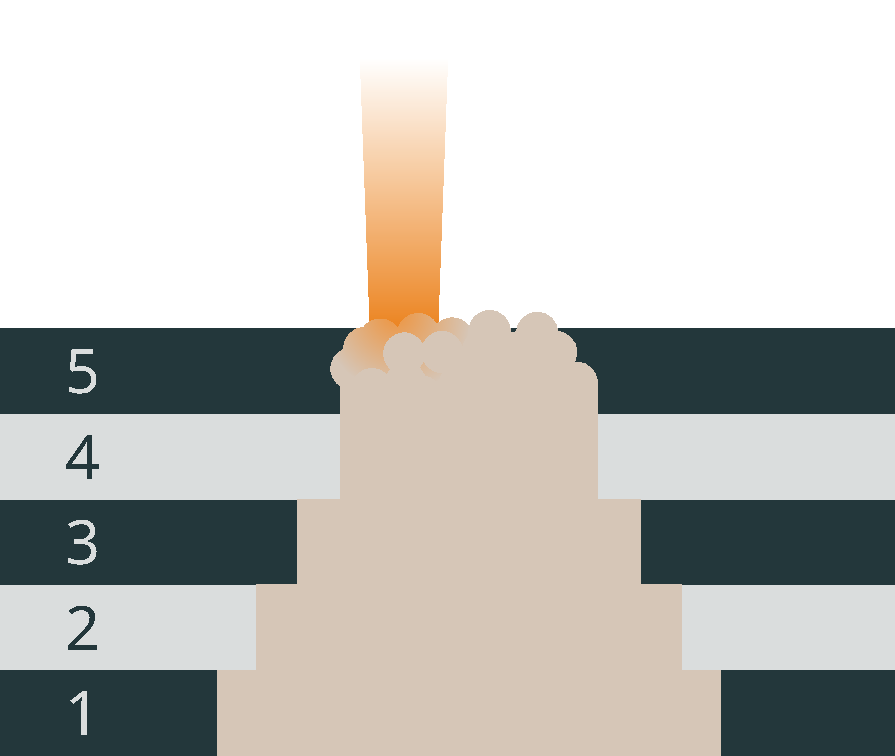
\includegraphics[width=0.5\textwidth]{Pictures/Vector/PDF/SLS_scheme.pdf}
    %\end{figure}
    %}
  
  \end{frame}
  \subsection{Scelta del biopolimero}
  \begin{frame}{Scelta del biopolimero}
    \onslide<1>{
      \begin{center}
        \alert<1>{Quale biopolimero scegliere?}
      \end{center}
    }
    \onslide*<2>{
      \begin{center}
        Finestra di \textbf{sinterizzazione}
      \end{center}
    }
    %\onslide*<2>{Finestra di sinterizzazione}

    \onslide*<3>{
      \begin{center}
        Finestra di \alert{sinterizzazione} \\ 
        \vspace{1 cm}
        Range di temperatura tra la \textbf{cristallizzazione} e la \textbf{fusione} del polimero
      \end{center}
    }

    \onslide*<4->{
      \begin{center}
        \textbf{\alert<4>{PHBH}} \\ 
        \vspace{1 cm}
        (poly)-hydroxy-3-butyrate-3-hexanoate
      \end{center}
    }

    \onslide*<5>{
      \begin{figure}[h]
        \centering
        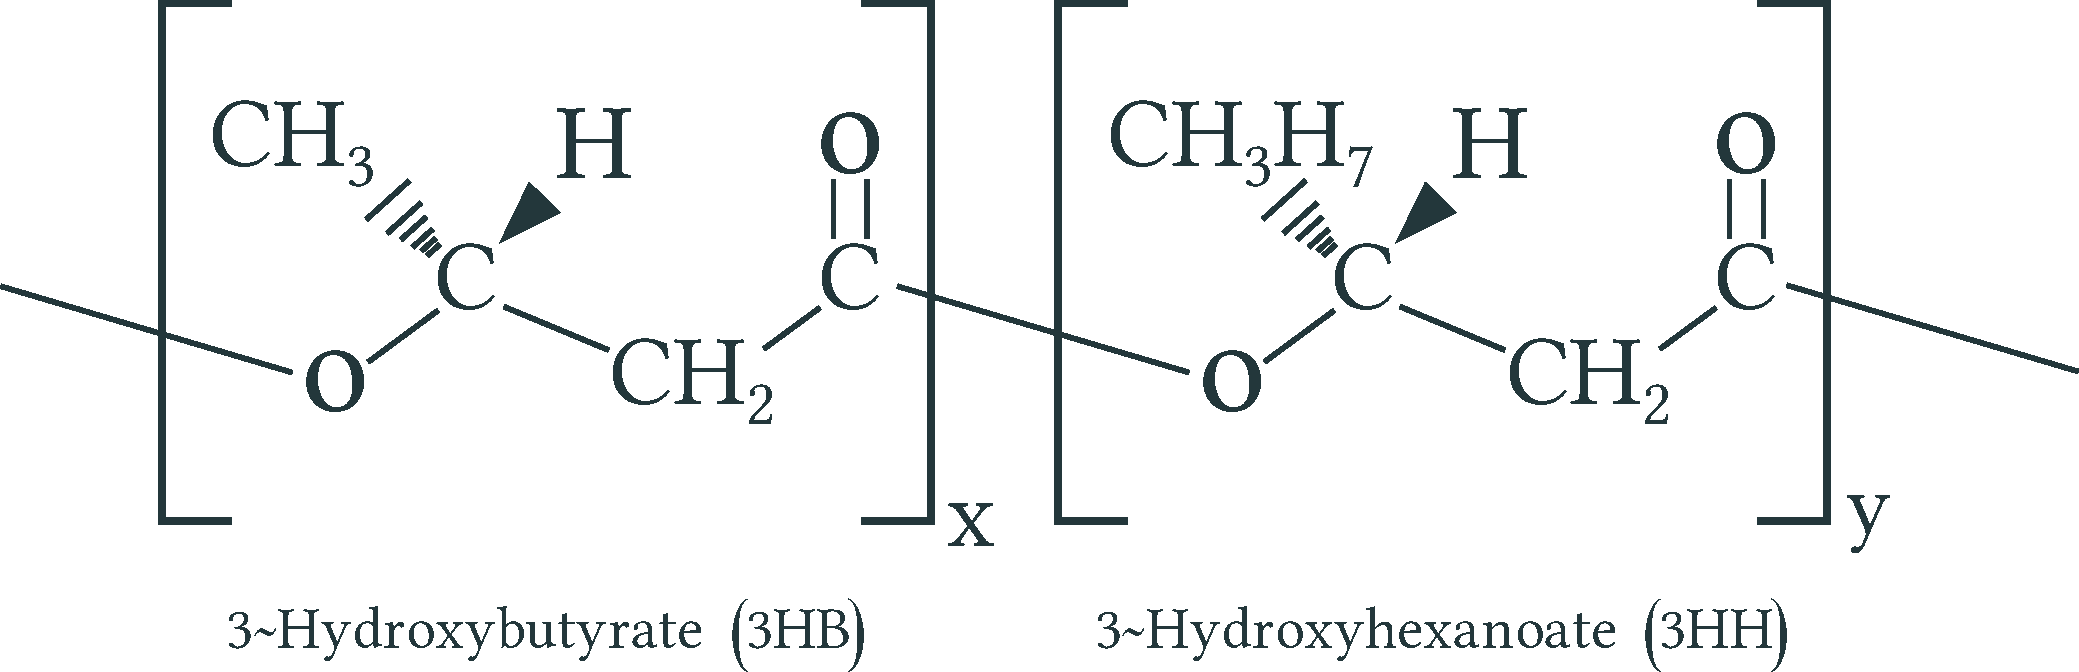
\includegraphics[width=0.5\textwidth]{Pictures/Vector/PDF/phbh_molecule.pdf}
        
      \end{figure}
    }

    \onslide*<6>{
      %\begin{center}
          Copolimero della famiglia dei poliidrossialcanoati (PHA), con la più ampia finestra di sinterizzazione e potenziale per SLS
      %\end{center}
    }
  \end{frame}
\section{Produzione della polvere}

    \begin{frame}{Produzione della polvere}
        \onslide<1>{
          \begin{center}
            \alert<1>{Come si ottiene la polvere?}
          \end{center}
        }
        \onslide<2-3>{
          \begin{center}
            \textbf{Precipitazione chimica}
          \end{center}
        }

        \onslide*<3>{
          
          \begin{figure}[h!]
            \centering
            \includegraphics[width=0.3\textwidth]{Pictures/Vector/PDF/flask.pdf}
          \end{figure}
          
        }

        \onslide<4-7>{
          \begin{center}
            \alert<4>{Quali sono i vantaggi?}
          \end{center}
        }
        \begin{itemize}
          \item <5-7> \textbf{Rendimenti più alti} rispetto alla macinatura criogenica
          \item <6-7> Polveri con una \textbf{distribuzione} di dimensioni più \textbf{uniforme}
          \item <7> Polveri con \textbf{morfologia} adeguata per l'\textbf{SLS}
        \end{itemize}
        
      \end{frame}

      \begin{frame}
        \frametitle{Precipitazione chimica}
      
        
        
        \onslide*<1>{
          \begin{figure}[h]
            \centering
            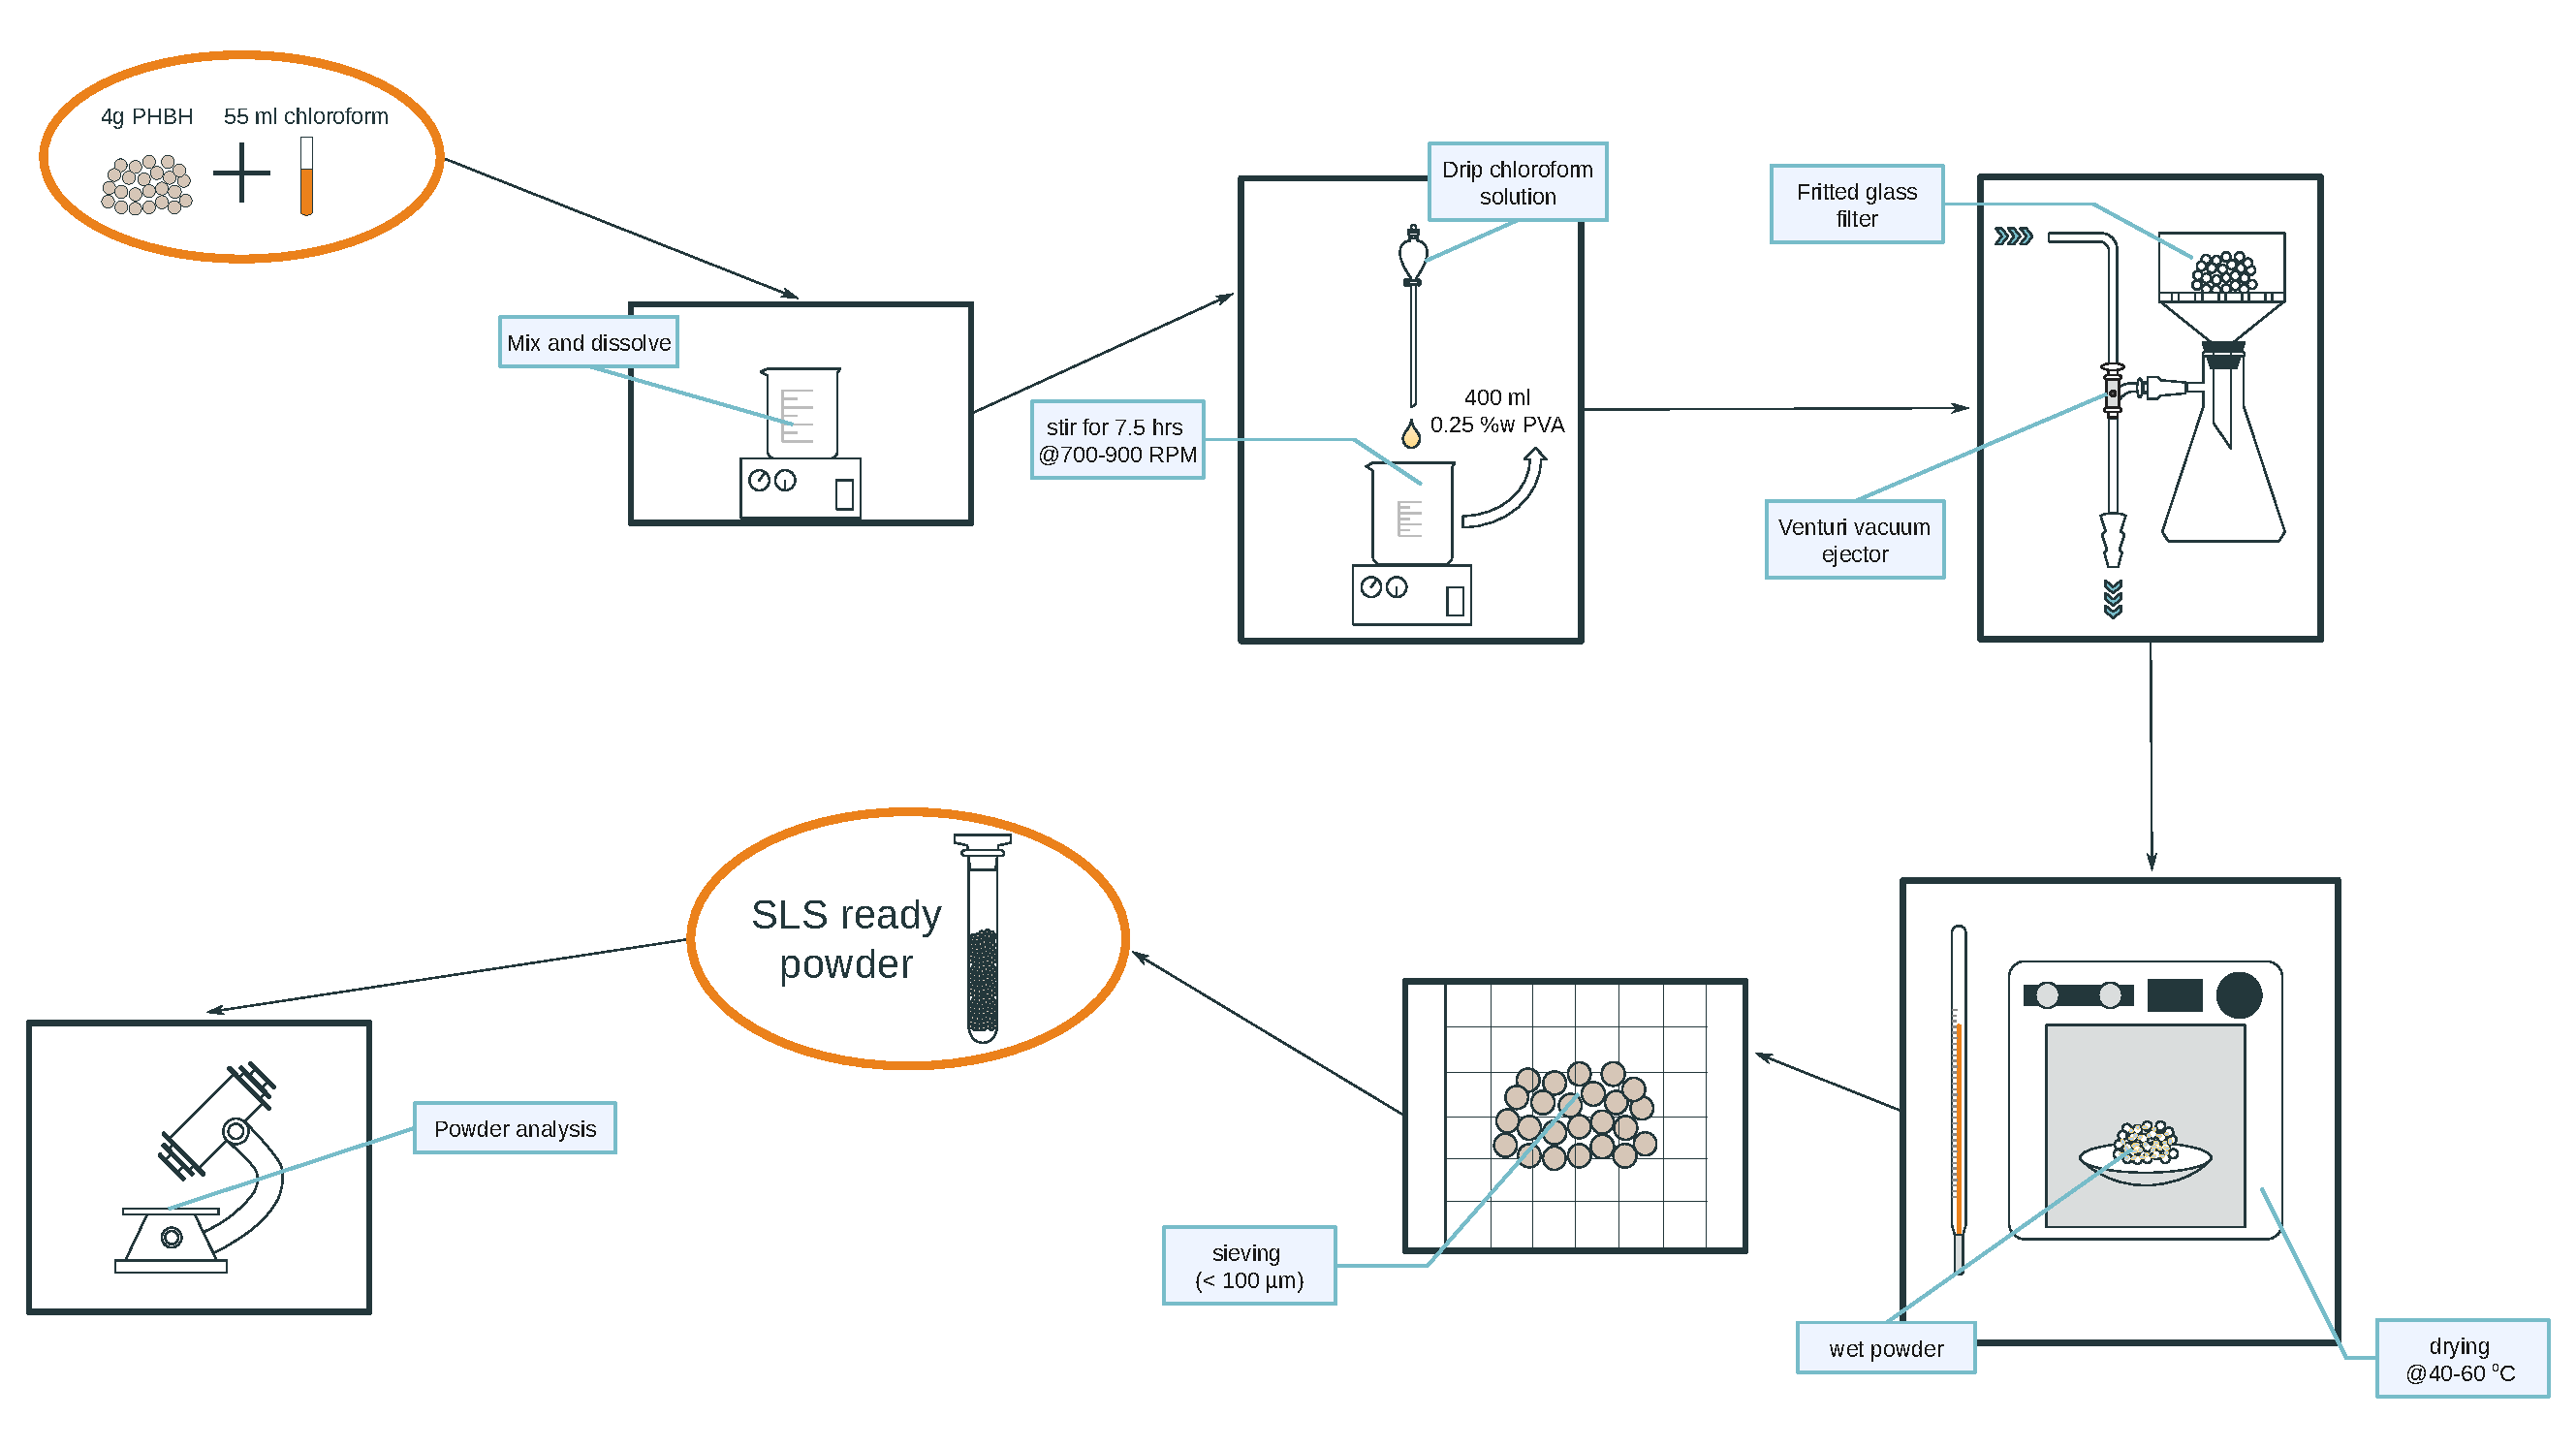
\includegraphics[width=0.8\textwidth]{Pictures/Vector/PDF/process_diagram_readapted.pdf}

          \end{figure}
        }
        \onslide*<2>{
          \begin{figure}[h]
            \centering
            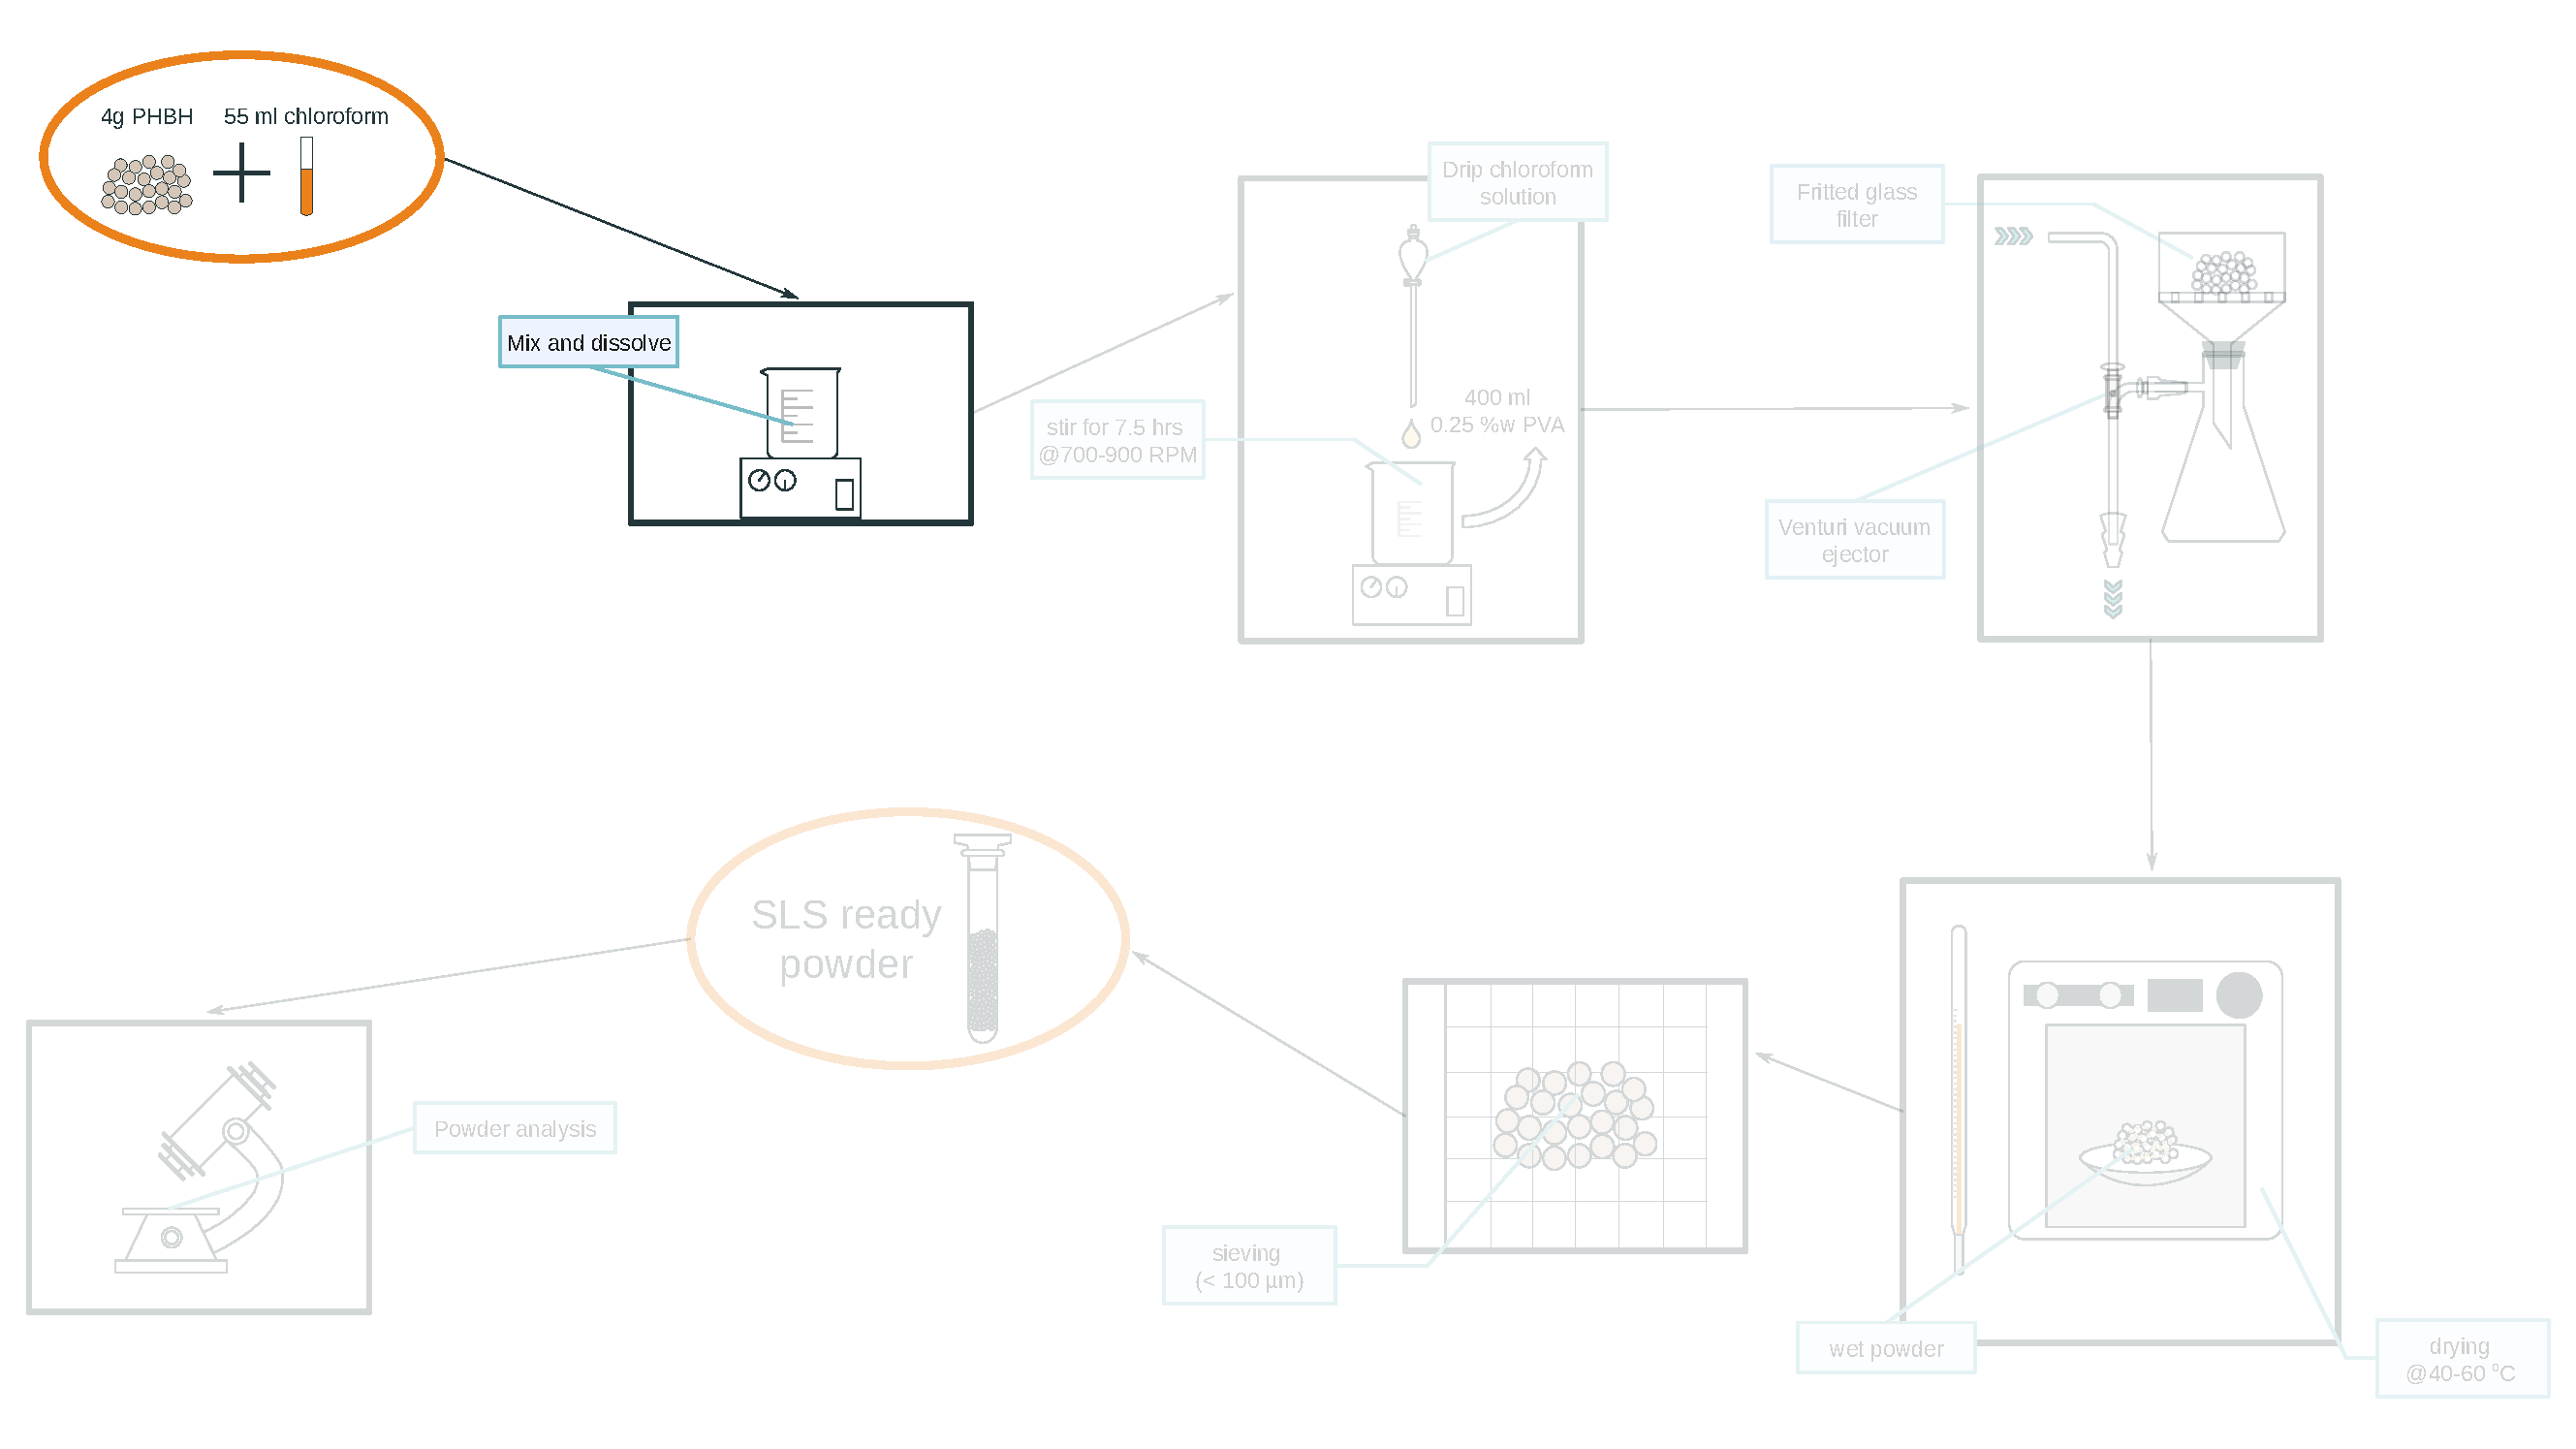
\includegraphics[width=0.8\textwidth]{Pictures/Vector/PDF/process_diagram_readapted-step1.pdf}

          \end{figure}
        }        
        \onslide*<3>{
          \begin{figure}[h]
            \centering
            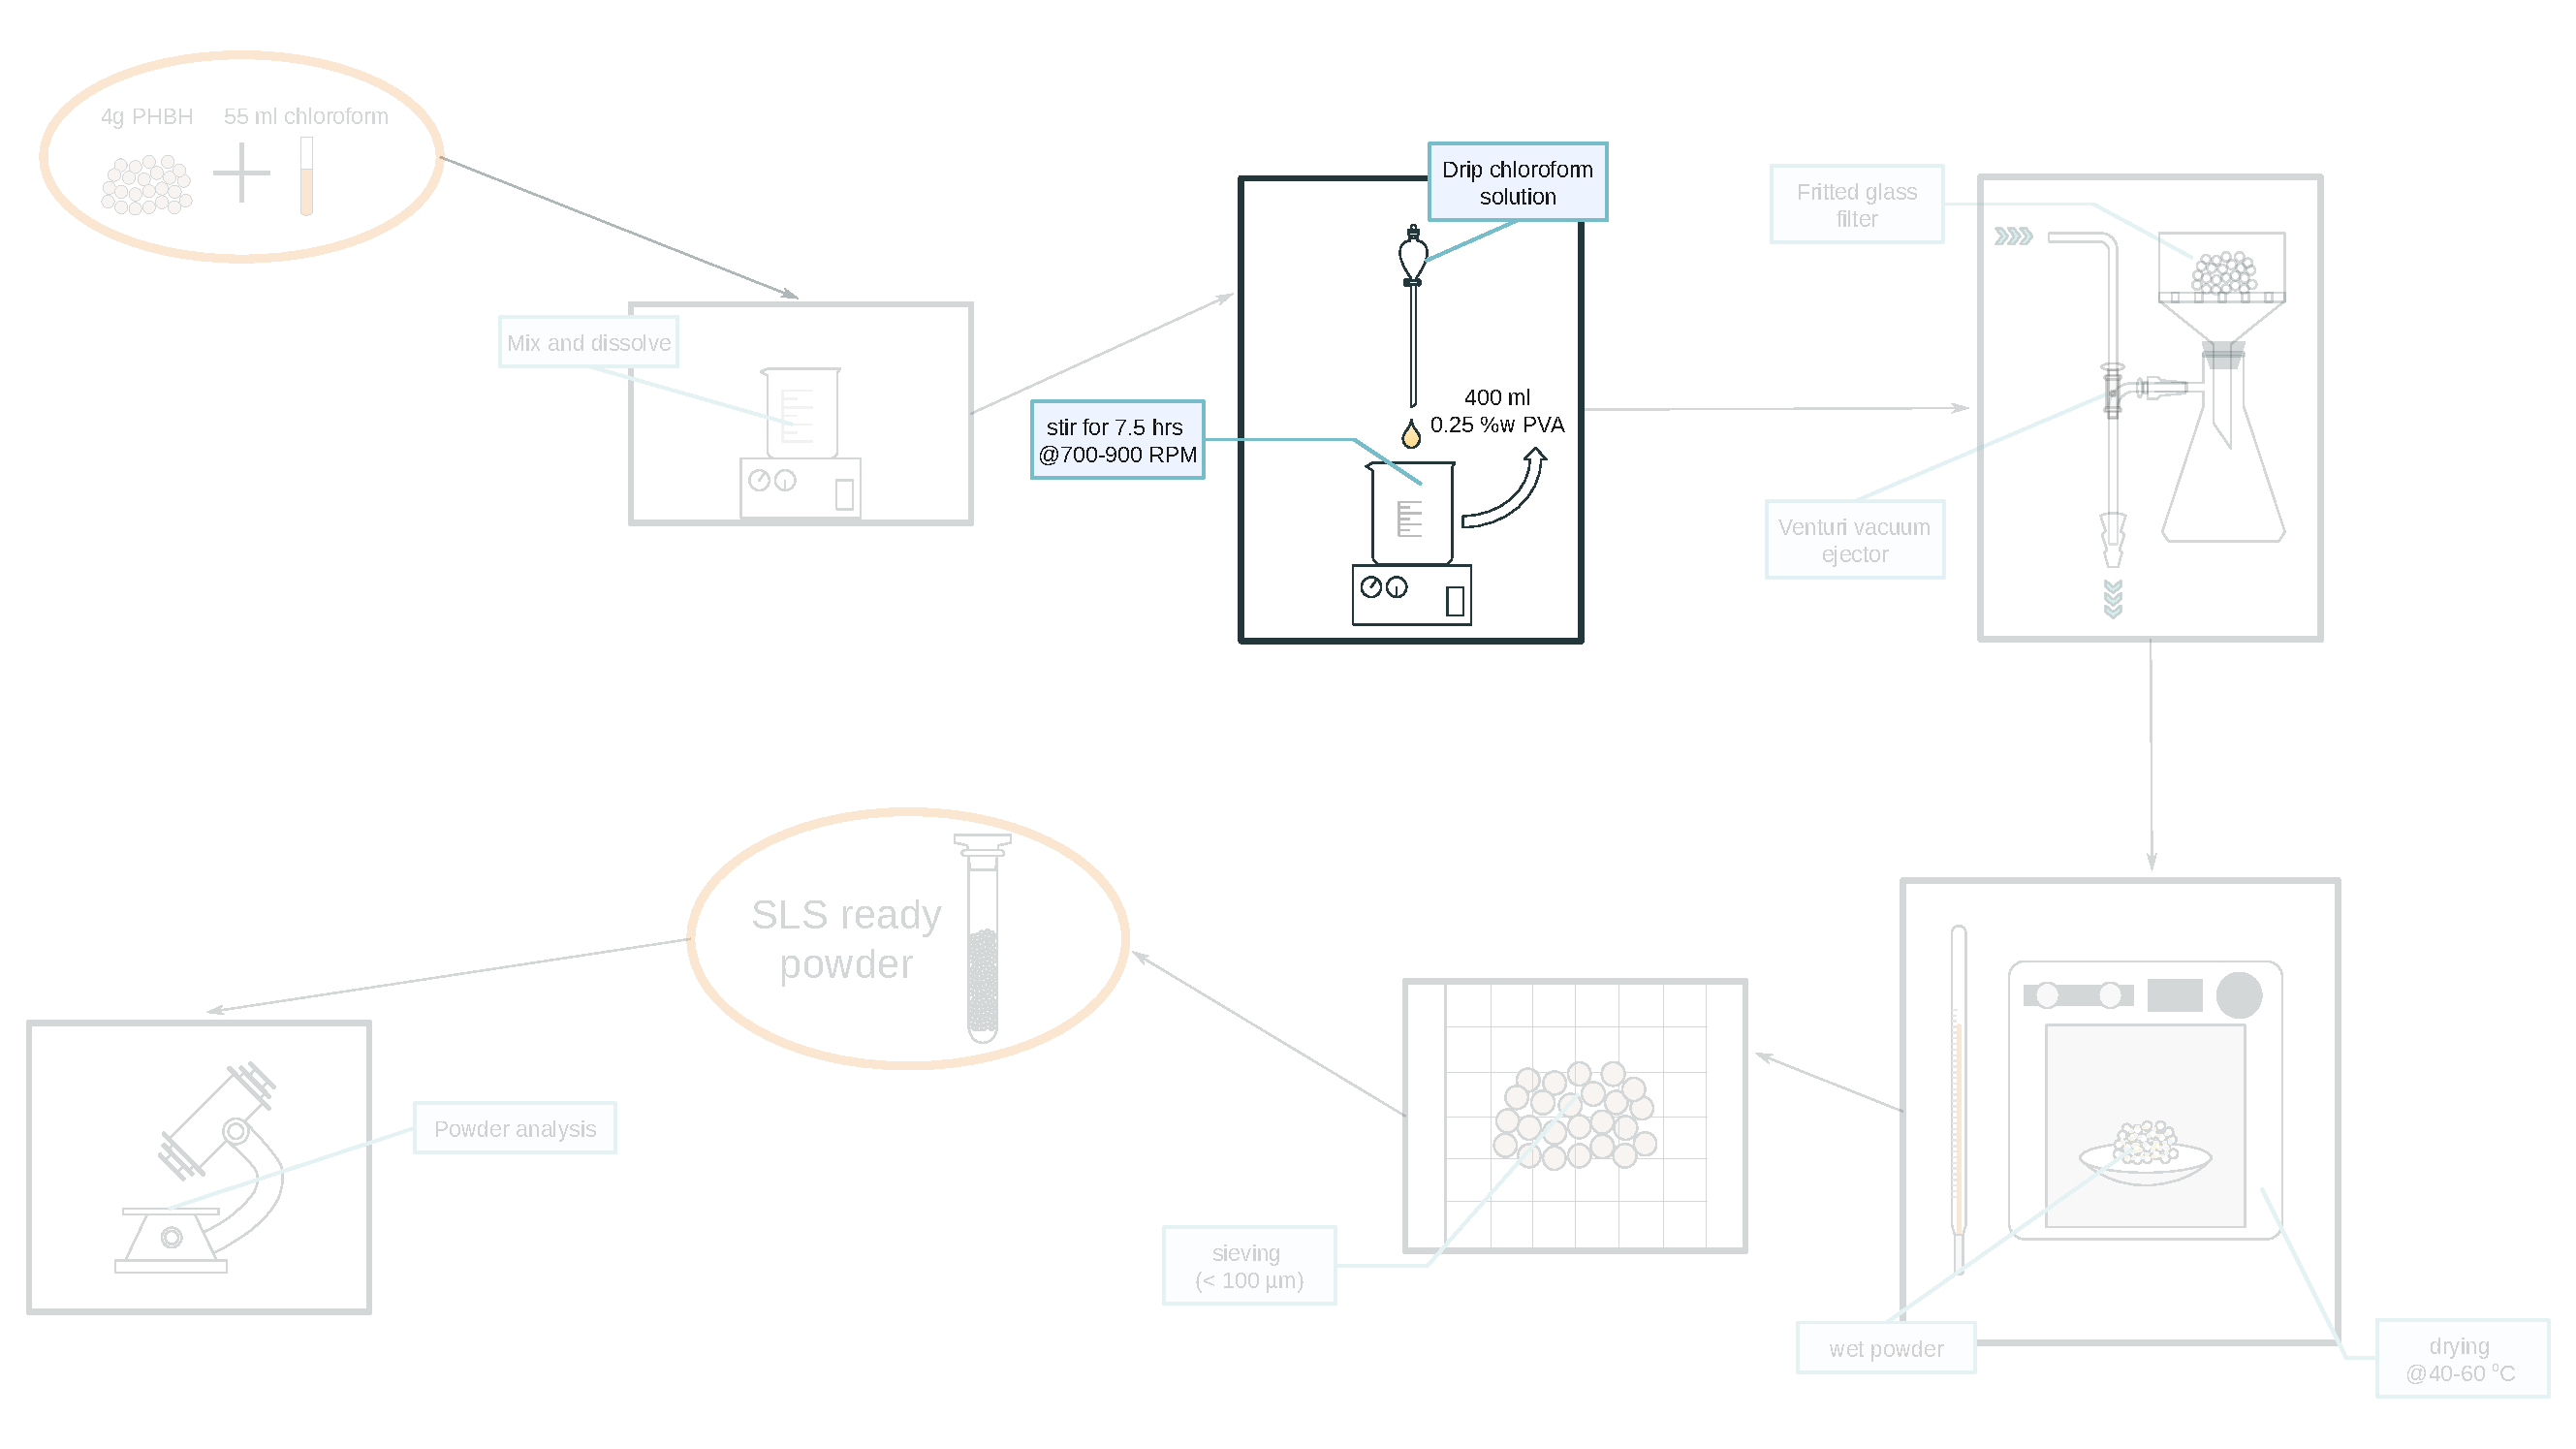
\includegraphics[width=0.8\textwidth]{Pictures/Vector/PDF/process_diagram_readapted-step2.pdf}

          \end{figure}
        }
        \onslide*<4>{
          \begin{figure}[h]
            \centering
            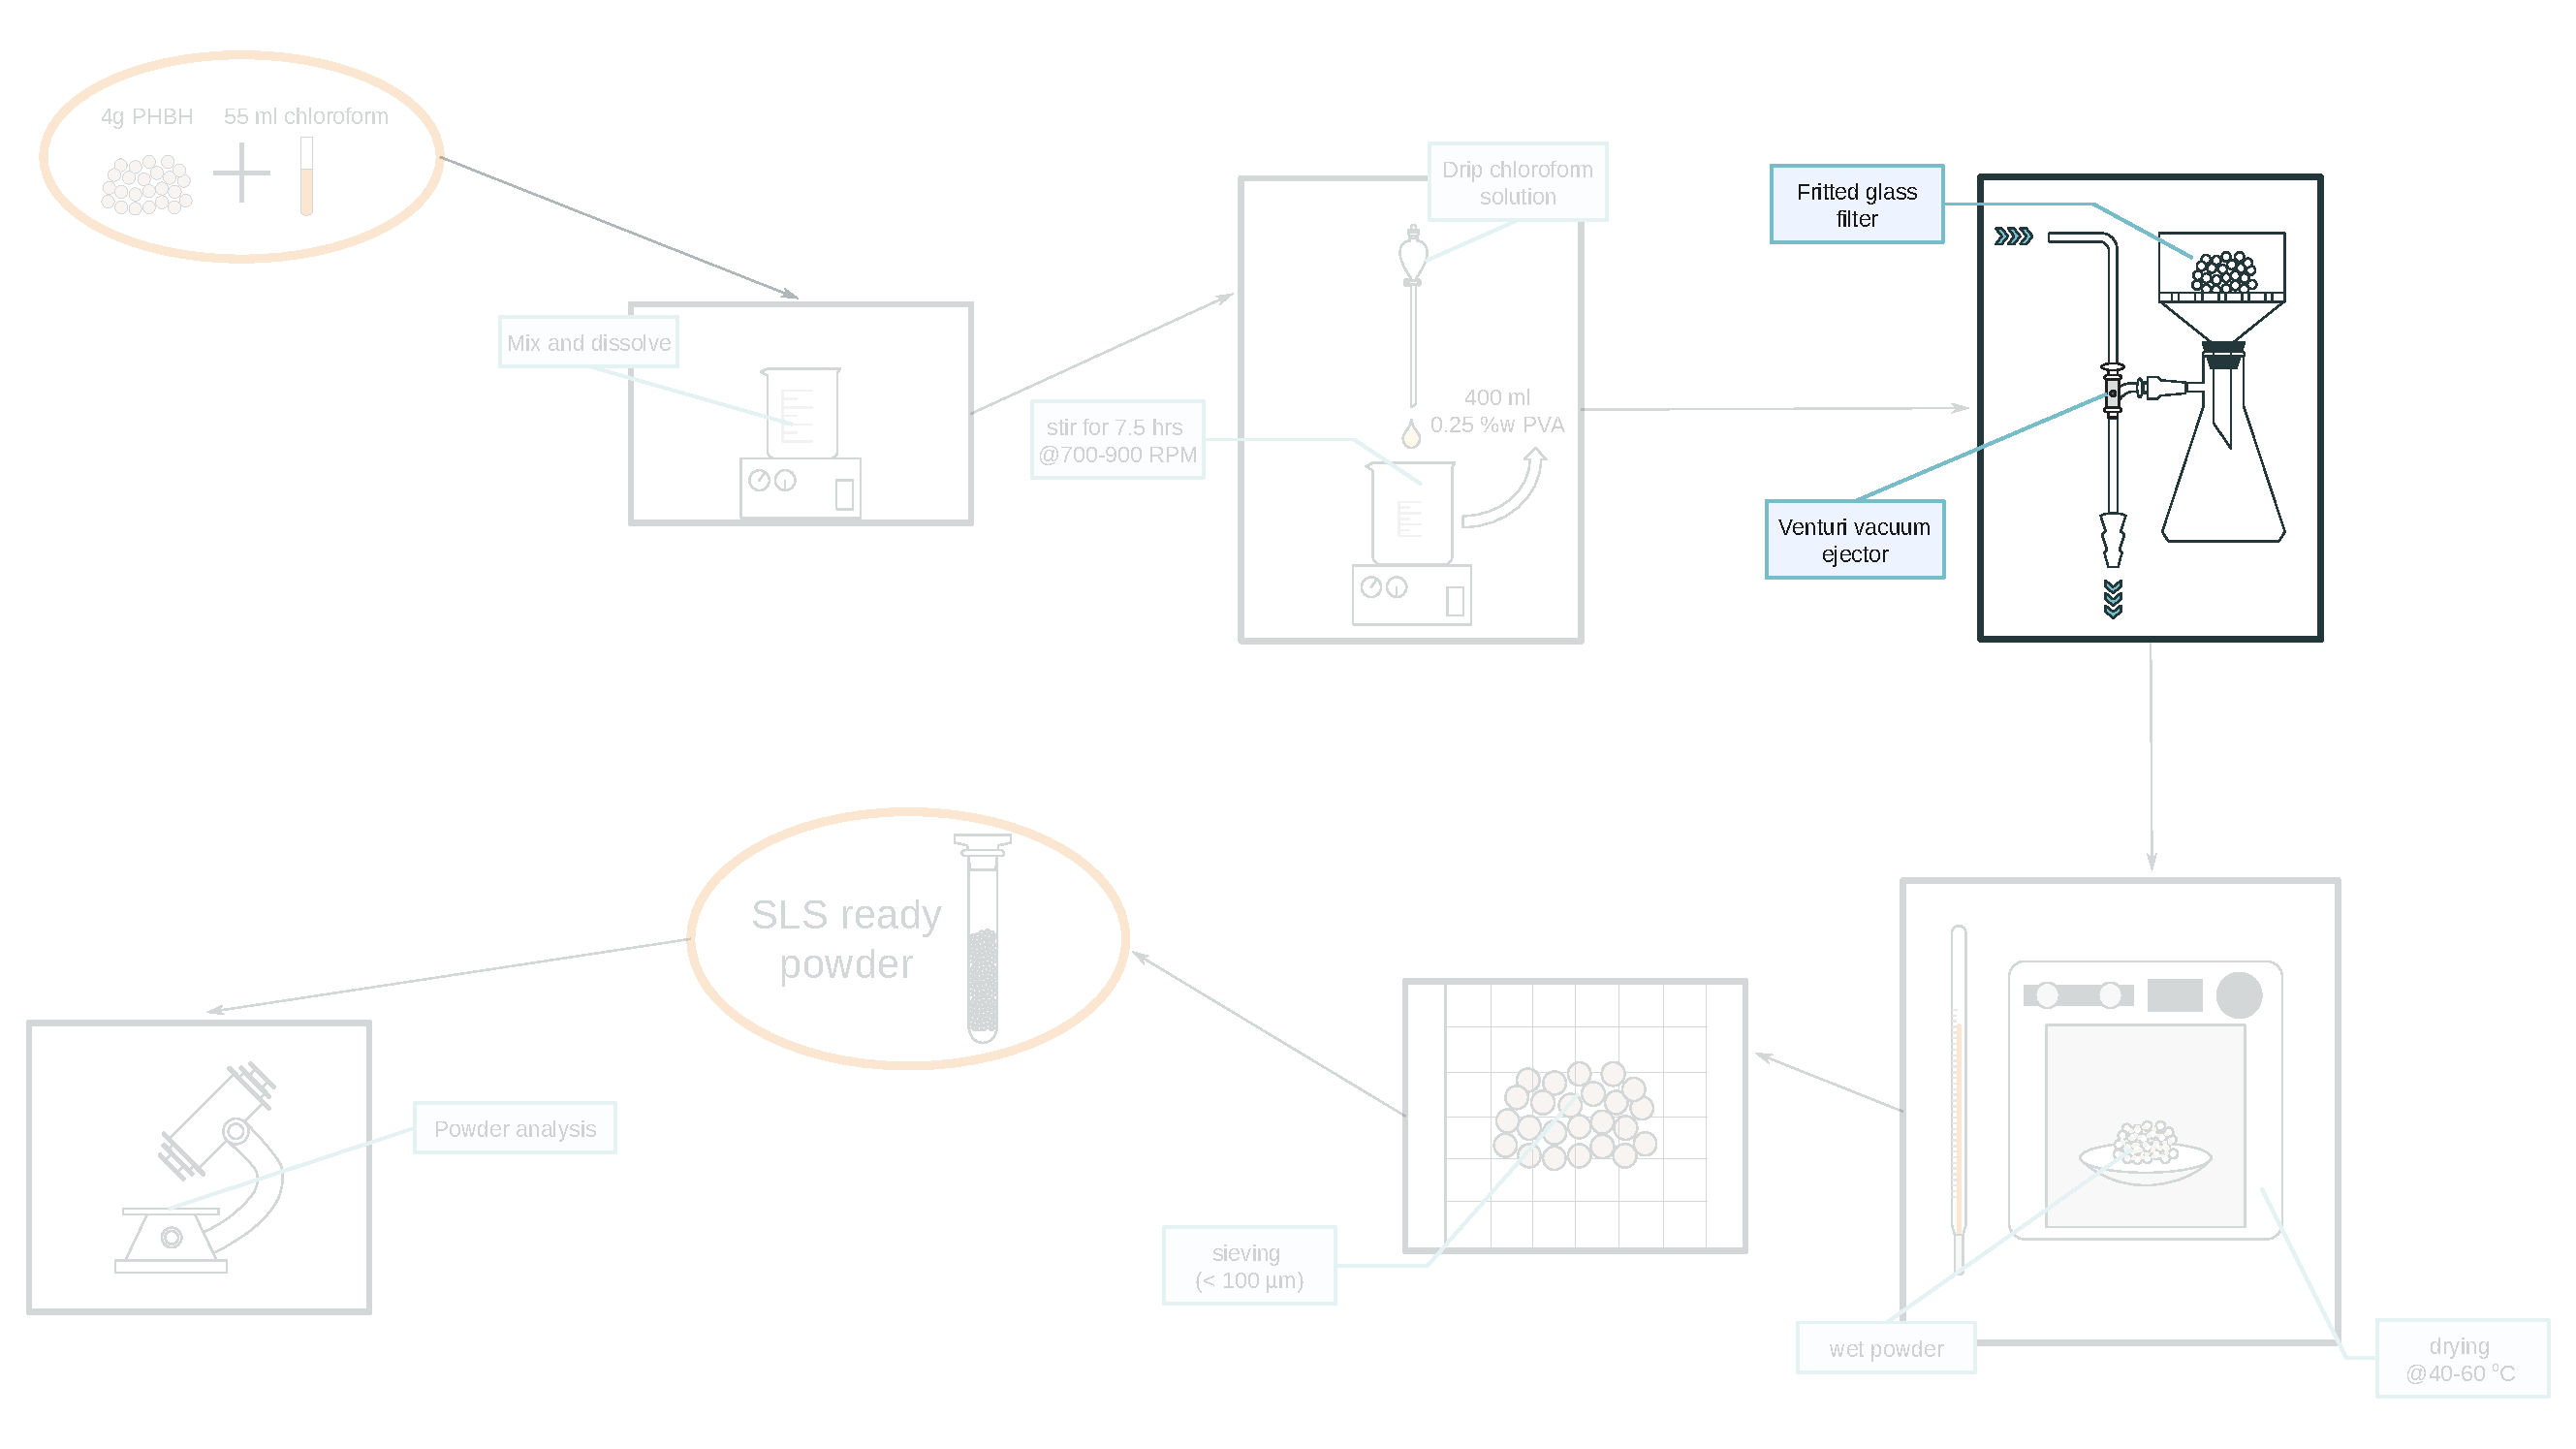
\includegraphics[width=0.8\textwidth]{Pictures/Vector/PDF/process_diagram_readapted-step3.pdf}

          \end{figure}
        }
        \onslide*<5>{
          \begin{figure}[h]
            \centering
            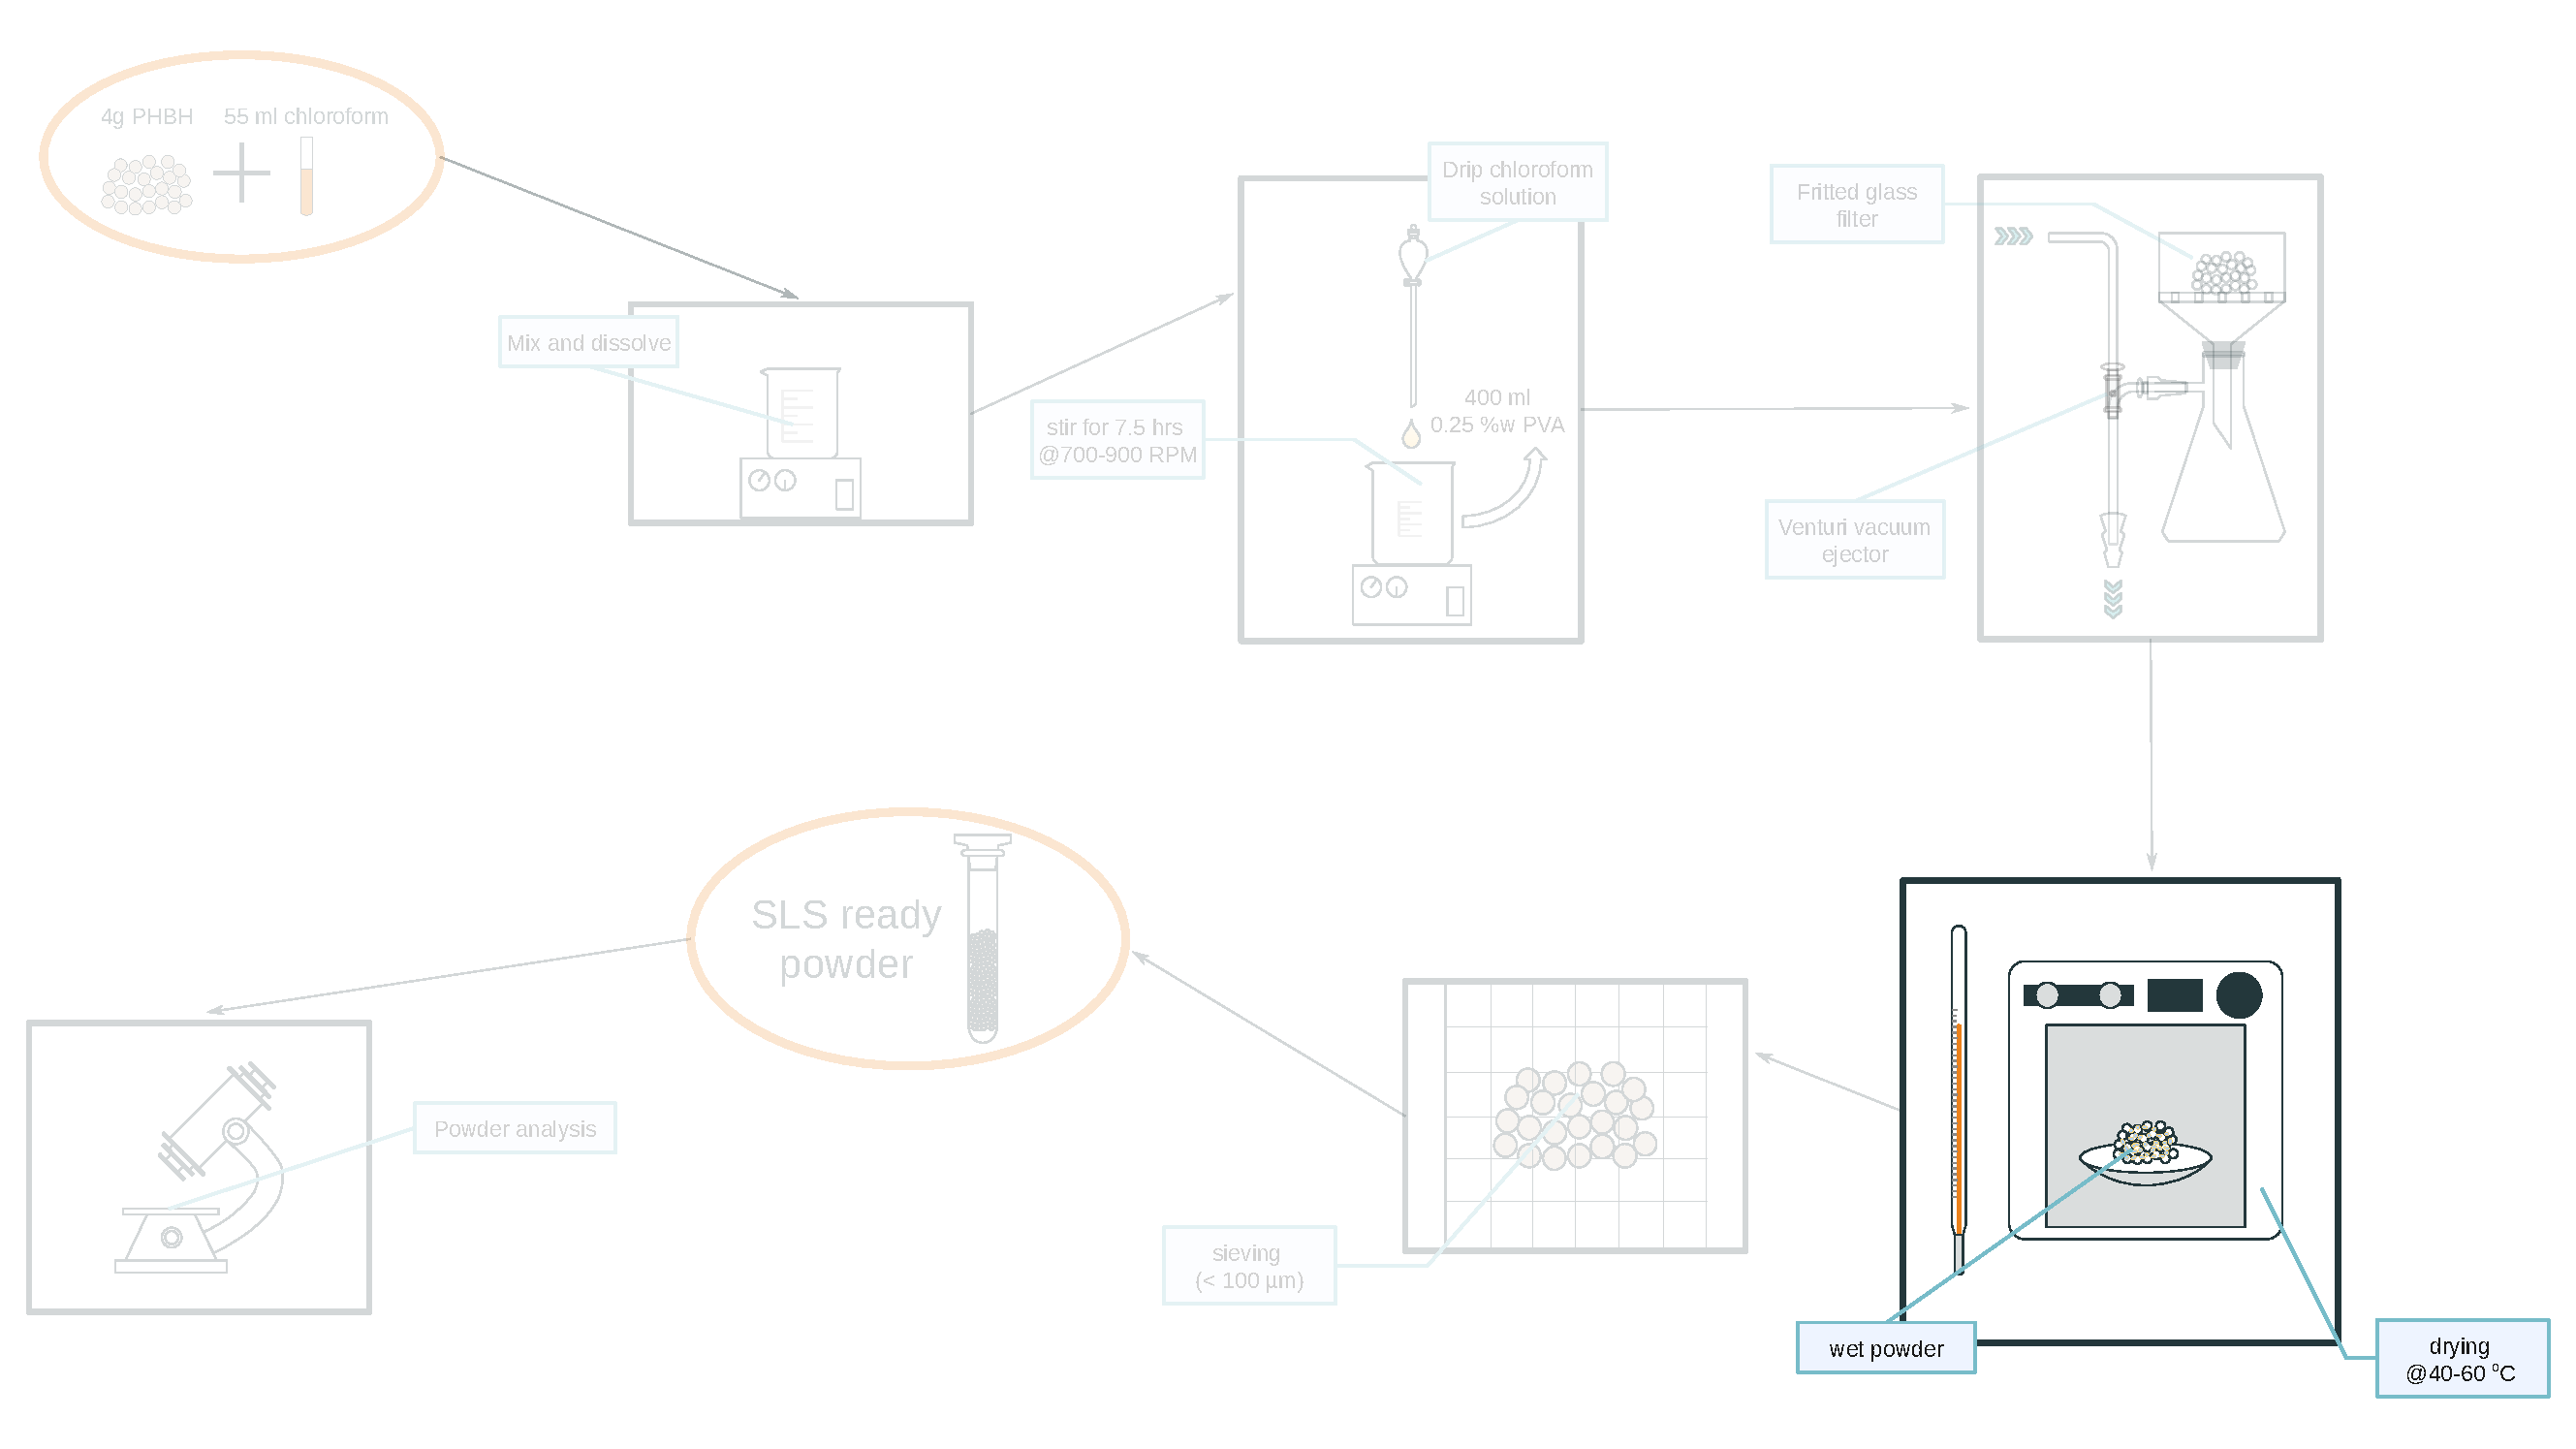
\includegraphics[width=0.8\textwidth]{Pictures/Vector/PDF/process_diagram_readapted-step4.pdf}

          \end{figure}
        }
        \onslide*<6>{
          \begin{figure}[h]
            \centering
            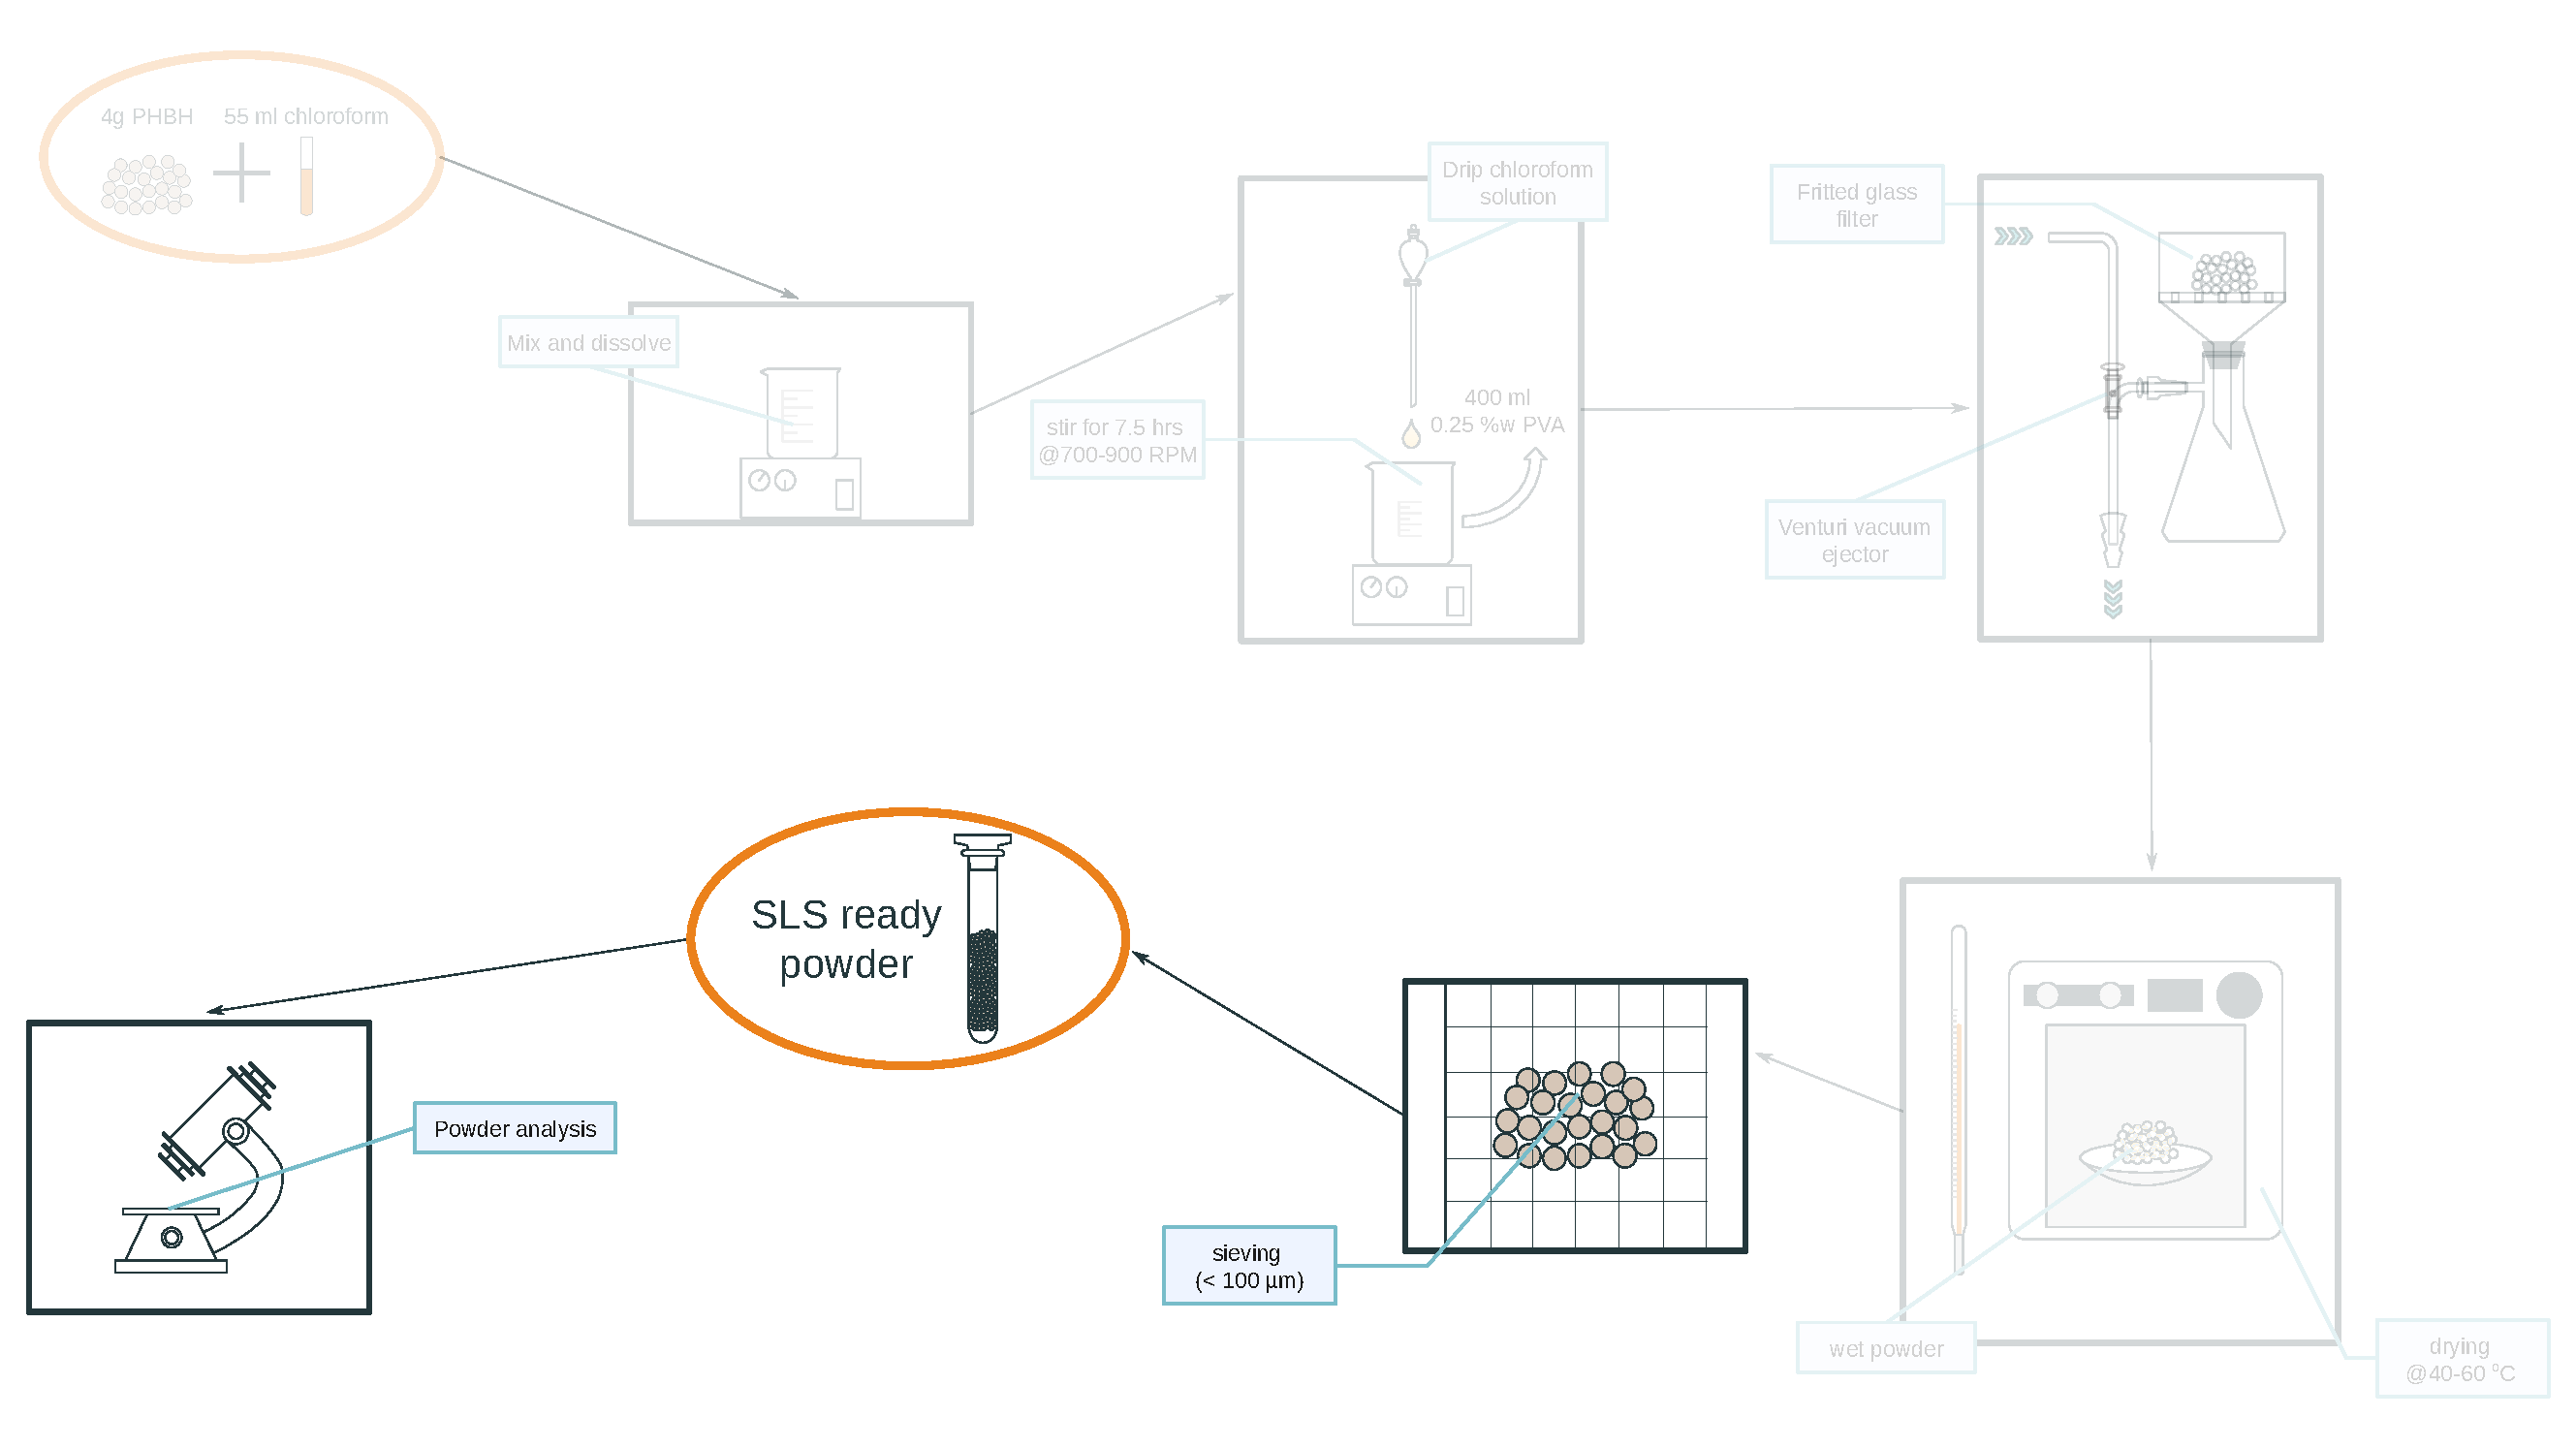
\includegraphics[width=0.8\textwidth]{Pictures/Vector/PDF/process_diagram_readapted-step5.pdf}

          \end{figure}
        }
        \onslide*<7>{
          \begin{center}
            \alert{Qual è la resa del processo di precipitazione?}
          \end{center}
        }
        \onslide*<8->{
          
          \begin{figure}[h!]
            \centering
            \begin{tikzpicture}
              \begin{axis}[
                mbarplot,
                bar width=20pt,
                ylabel={Total yield $[\%]$},
                %xlabel={Pellet to powder yield},
                title={Pellet to powder yield},
                width=0.65\textwidth,
                height=6cm,
                xmax = 0.1,
                xmin = -0.1,
                xticklabels={},
                xtick={0},
                legend style={anchor=north west},
                nodes near coords,
              ]
        
              \onslide*<8->{\addplot plot coordinates {(-0.01, 1)};} 
              \onslide*<9->{\addplot plot coordinates {(0, 30)};}    
              \onslide*<10>{\addplot plot coordinates {(0.01, 75)};}
        
              \legend{Day 1, Previous research, Current}
        
              \end{axis}
            \end{tikzpicture}
          \end{figure}
            
            
            
          
        }
      \end{frame}
  \section{Caratterizzazione della polvere}

    \begin{frame}{Requisiti della polvere}
        \onslide*<1>{
        \begin{center}
          \alert<1>{Quali sono i requisiti fondamentali per una polvere SLS ready?}
        \end{center}  
        }

        \begin{itemize}
          \item <2->  \textbf{Granulometria}
          \item <3->  \textbf{Morfologia}
          \item <4>   \textbf{Stabilità termica}
          
          
        \end{itemize}

        \onslide*<2>{La polvere deve avere una distribuzione media tra \textbf{20 e 80 $\mu m$}}
        \onslide*<3>{Le particelle devono essere \textbf{sferiche}, non vuote, per consentire la formazione efficace di \textbf{colli di sinterizzazione}}
        \onslide*<4>{La polvere deve rimanere \textbf{termicamente inalterata} durante la stampa}

      \end{frame}




    \subsection{Microscopia a Scansione Elettronica}

    \begin{frame}
      \frametitle{Microscopia a Scansione Elettronica}

      \onslide*<1>{
        \begin{center}
          \alert<1>{Microscopia a Scansione Elettronica}
        \end{center}
      }

      \onslide*<2>{La microscopia a scansione elettronica (\textbf{SEM}) è un metodo di analisi che permette di ricostruire la morfologia di una superficie in 3D, sfruttando l'emissione di 
      \textbf{elettroni secondari} da un campione sottoposto ad un fascio di elettroni.}

      \onslide*<3>{
        \begin{figure}[h]
          \centering
          \includegraphics[width=0.9\textwidth]{Pictures/Vector/PDF/SEM_fake.pdf}
        \end{figure}
      }

      \onslide*<4>{
        \begin{center}
          \alert{Come dovrebbe apparire una polvere SLS ideale?}
        \end{center}
      }

      \onslide*<5>{
        \begin{figure}[h]
          \centering
          \caption{DALLE-2 Prompt: \textit{Round particles seen through a SEM microscope}}
          \includegraphics[width=0.4\textwidth]{Pictures/Vector/PDF/DALLE.pdf}
        \end{figure}
      }
      
      \onslide*<6>{

        \begin{figure}[h]
          \centering
          \caption{MAG: 461X}
          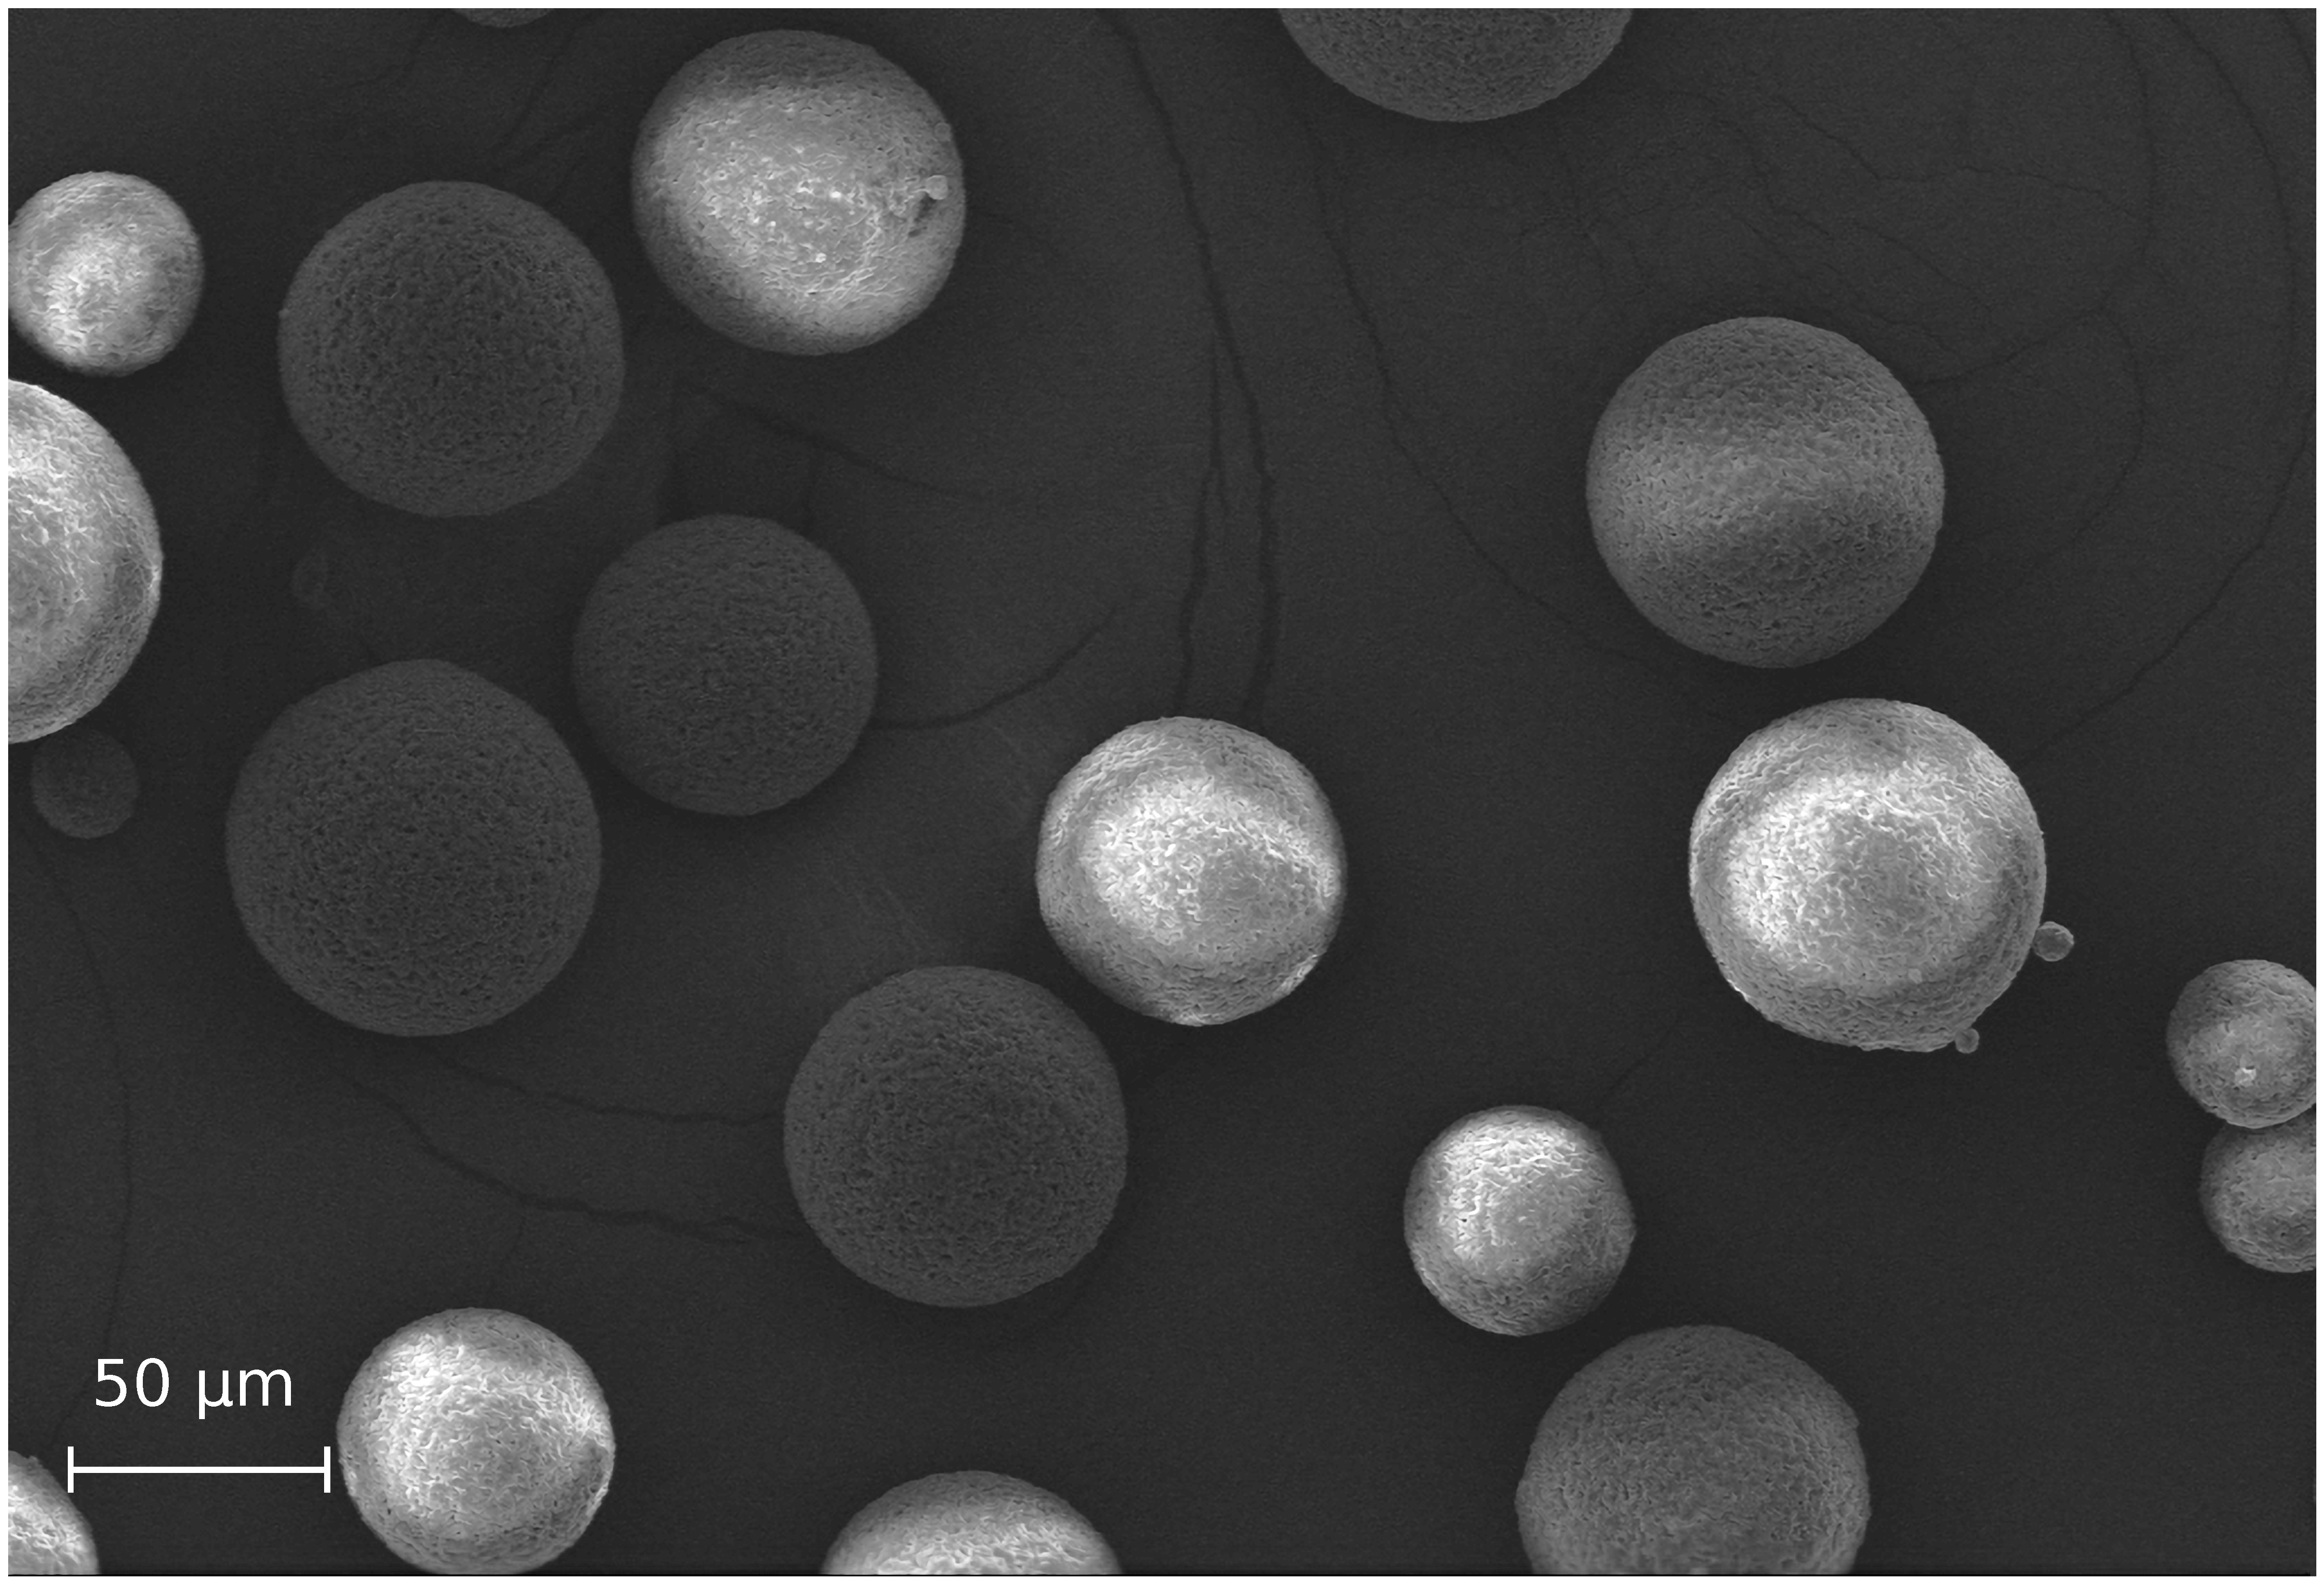
\includegraphics[width=0.6\textwidth]{Pictures/Vector/PDF/SEM/04_02.eps}
        \end{figure}
      }

      \onslide*<7>{
        \begin{figure}[h]
          \centering
          \caption{MAG: 400X}
          \includegraphics[width=0.6\textwidth]{Pictures/Vector/PDF/SEM/sample_06.eps}
        \end{figure}
      }

      \onslide*<8>{
        \begin{figure}[h]
          \centering
          \caption{MAG: 800X}
          \includegraphics[width=0.6\textwidth]{Pictures/Vector/PDF/SEM/sample_03.eps}
        \end{figure}
      }
      
          
    \end{frame}
    \subsection{Distribuzione granulometrica}

    \begin{frame}
      \frametitle{Distribuzione granulometrica}

      \onslide*<1>{
        \begin{center}
          \alert<1>{Qual è la distribuzione granulometrica della polvere ottenuta?}
        \end{center}
      }

      \onslide*<2>{La distribuzione ideale descritta in letteratura per la polvere SLS è tra \textbf{20} e \textbf{80 $\mu m$}}

      \onslide*<3>{I risultati ottenuti per \textbf{z-stack defocusing} di immagini in microscopia ottica (10X) confermano quanto già osservato con la microscopia a scansione elettronica}

      \onslide*<4>{
        \begin{figure}[h]
          \centering
          \caption{Particle size distribution}
          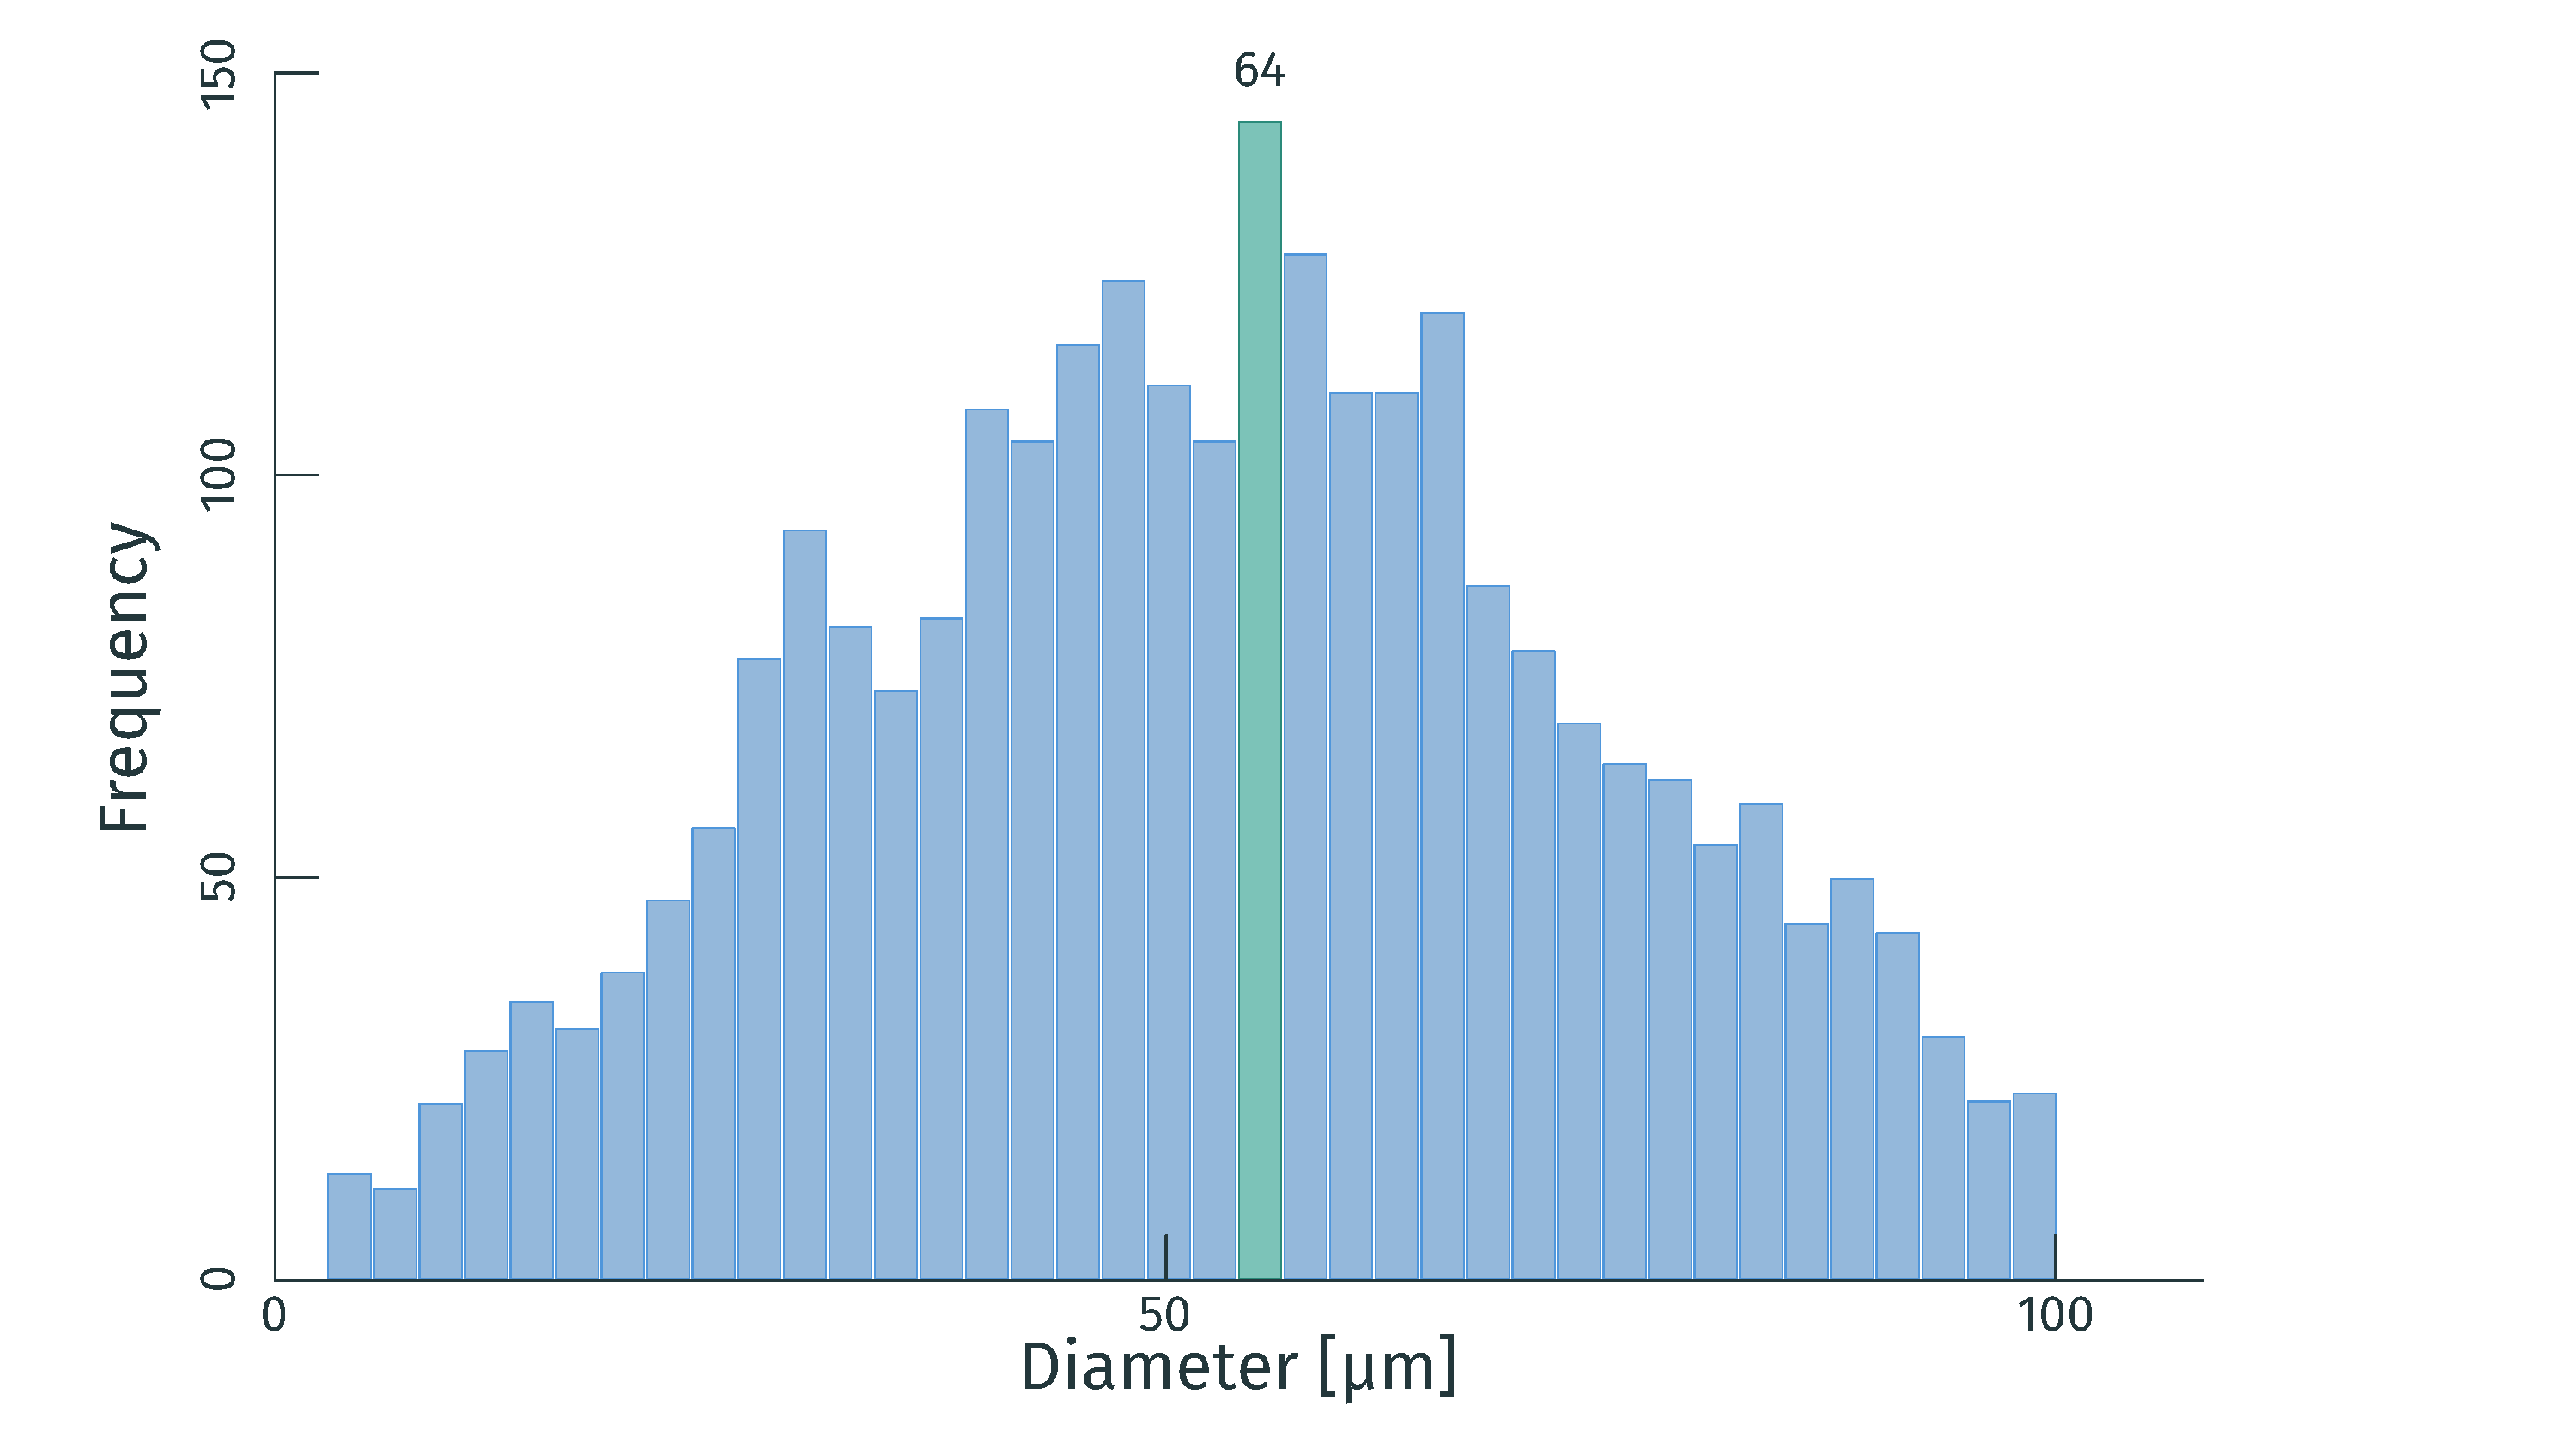
\includegraphics[width=0.8\textwidth]{Pictures/Vector/PDF/PSD.pdf}
        \end{figure}
      }

      \onslide*<5>{
        \begin{figure}[h]
          \centering
          \caption{Particle circularity}
          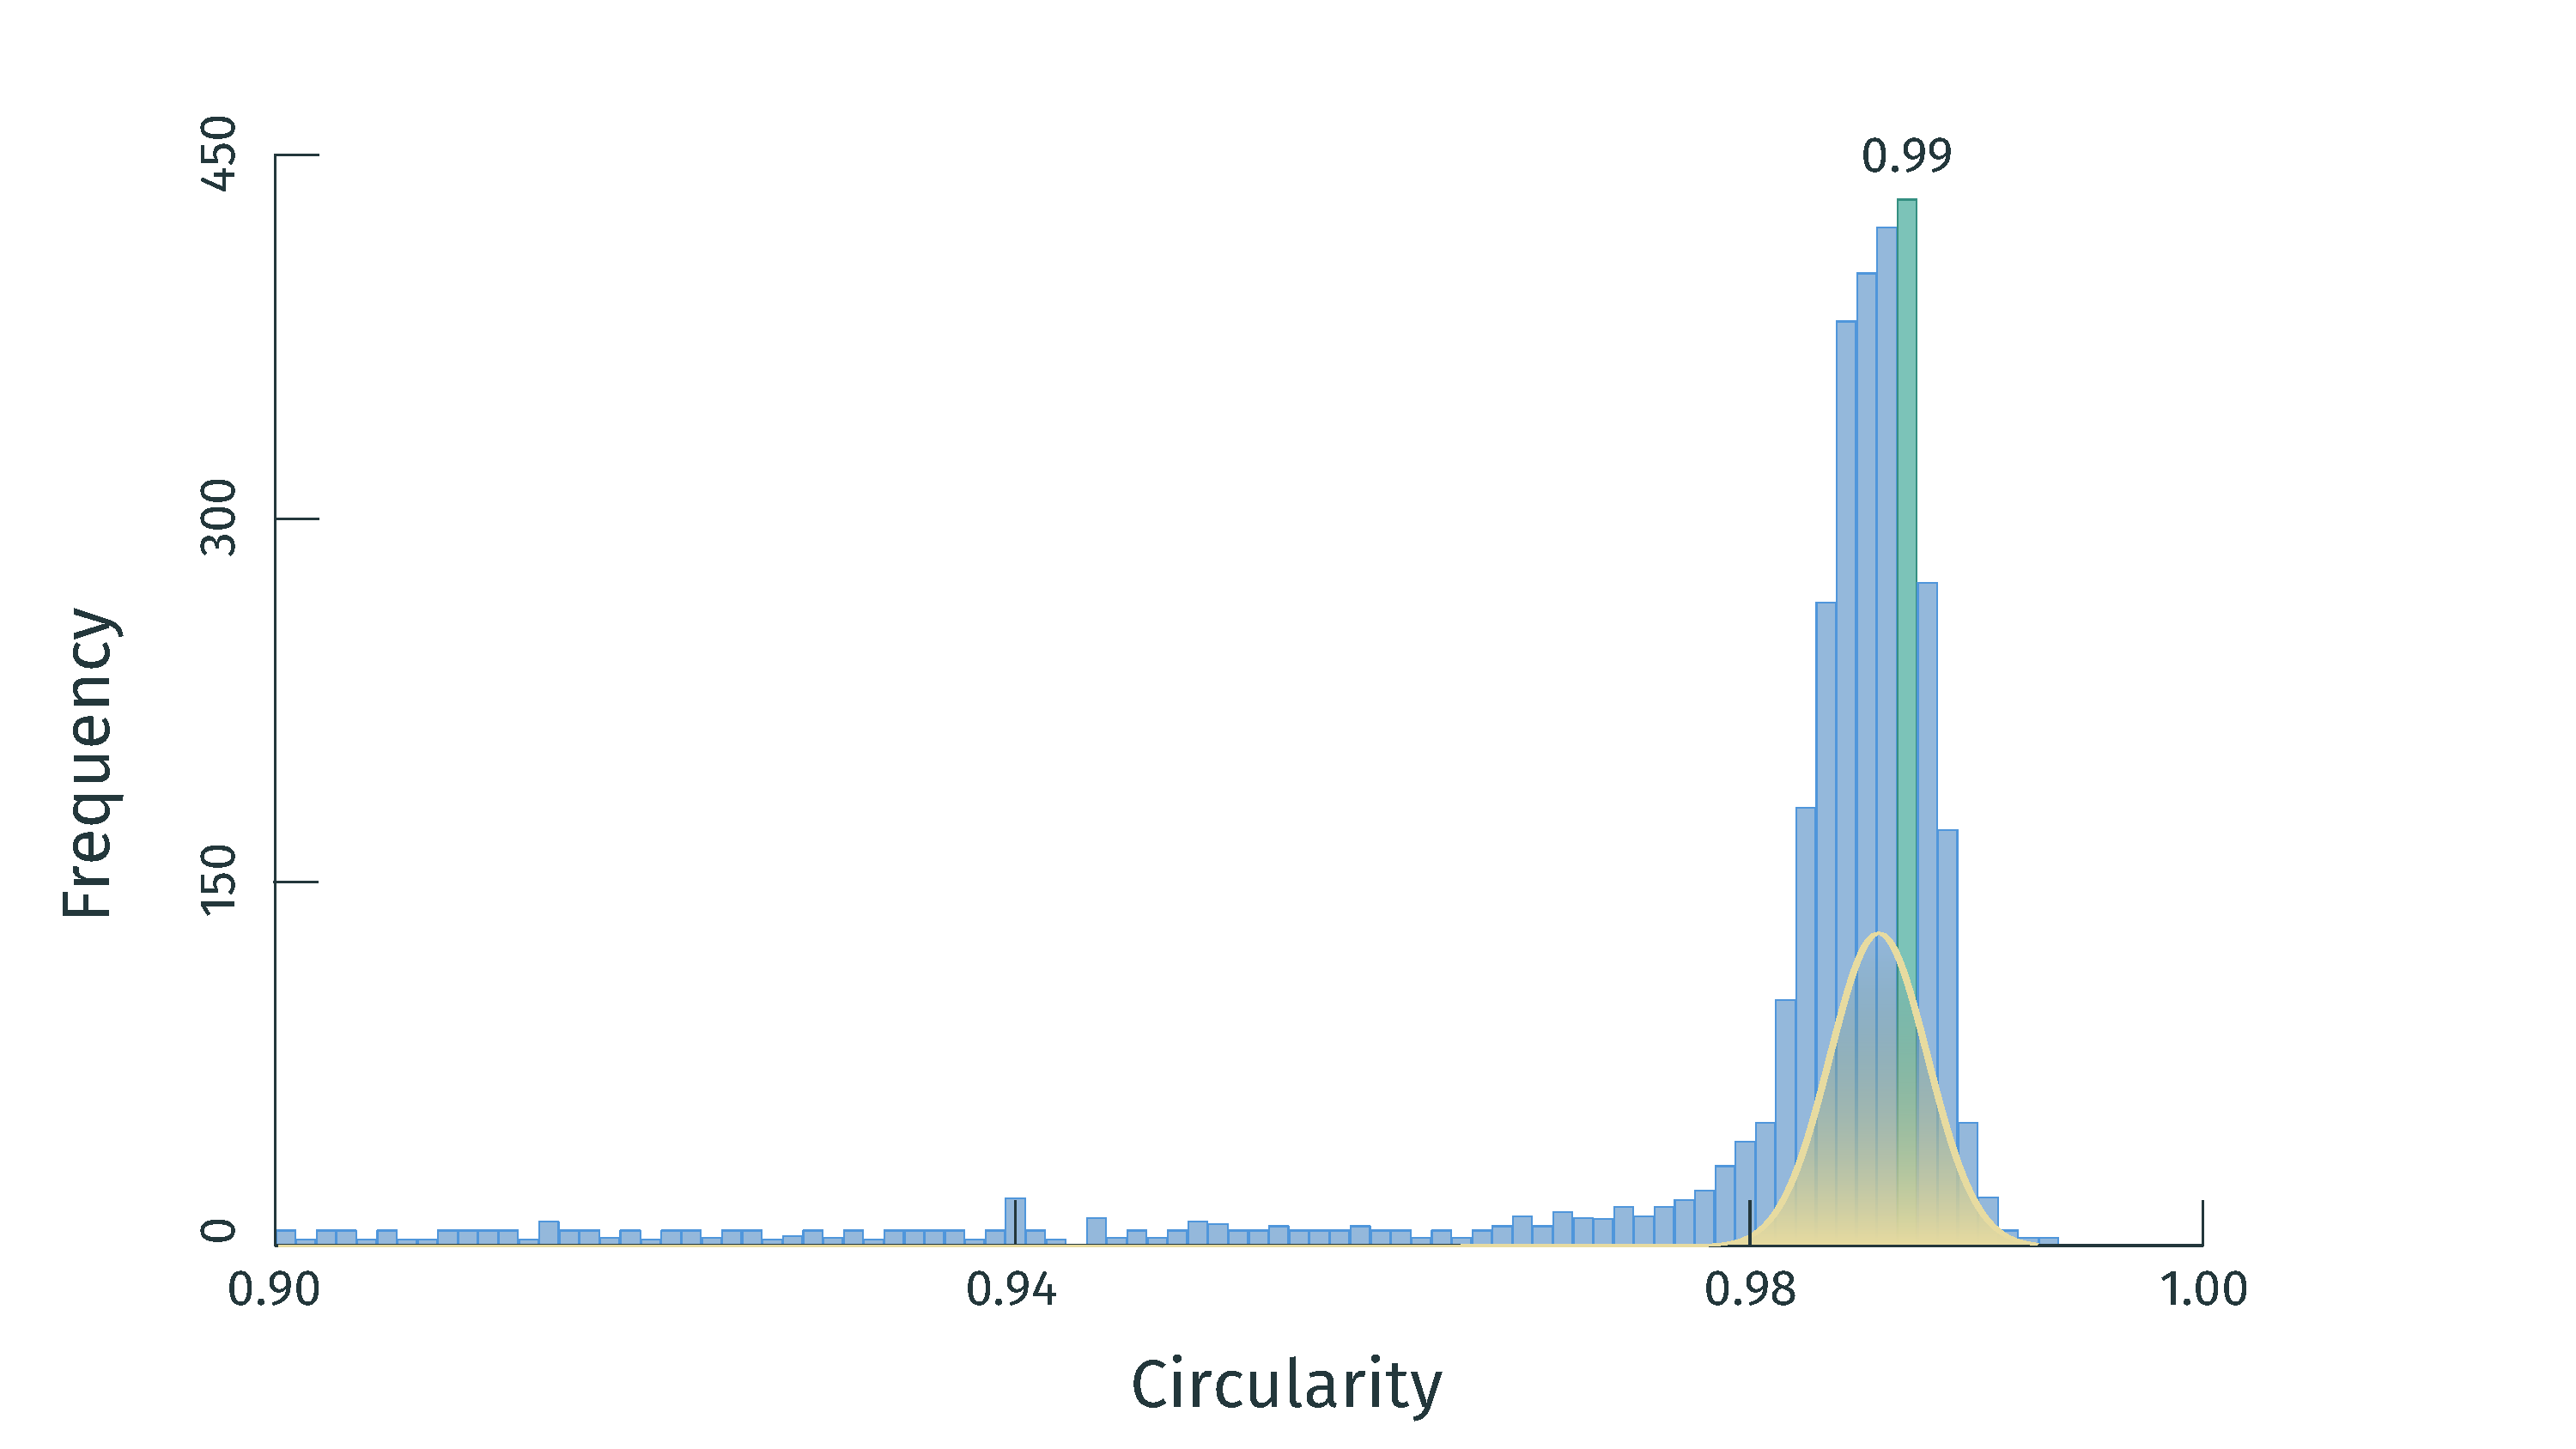
\includegraphics[width=0.8\textwidth]{Pictures/Vector/PDF/PSD_circularity-0.pdf}
        \end{figure}
      }

      \onslide*<6>{
        \begin{figure}[h]
          \centering
          \caption{Particle circularity}
          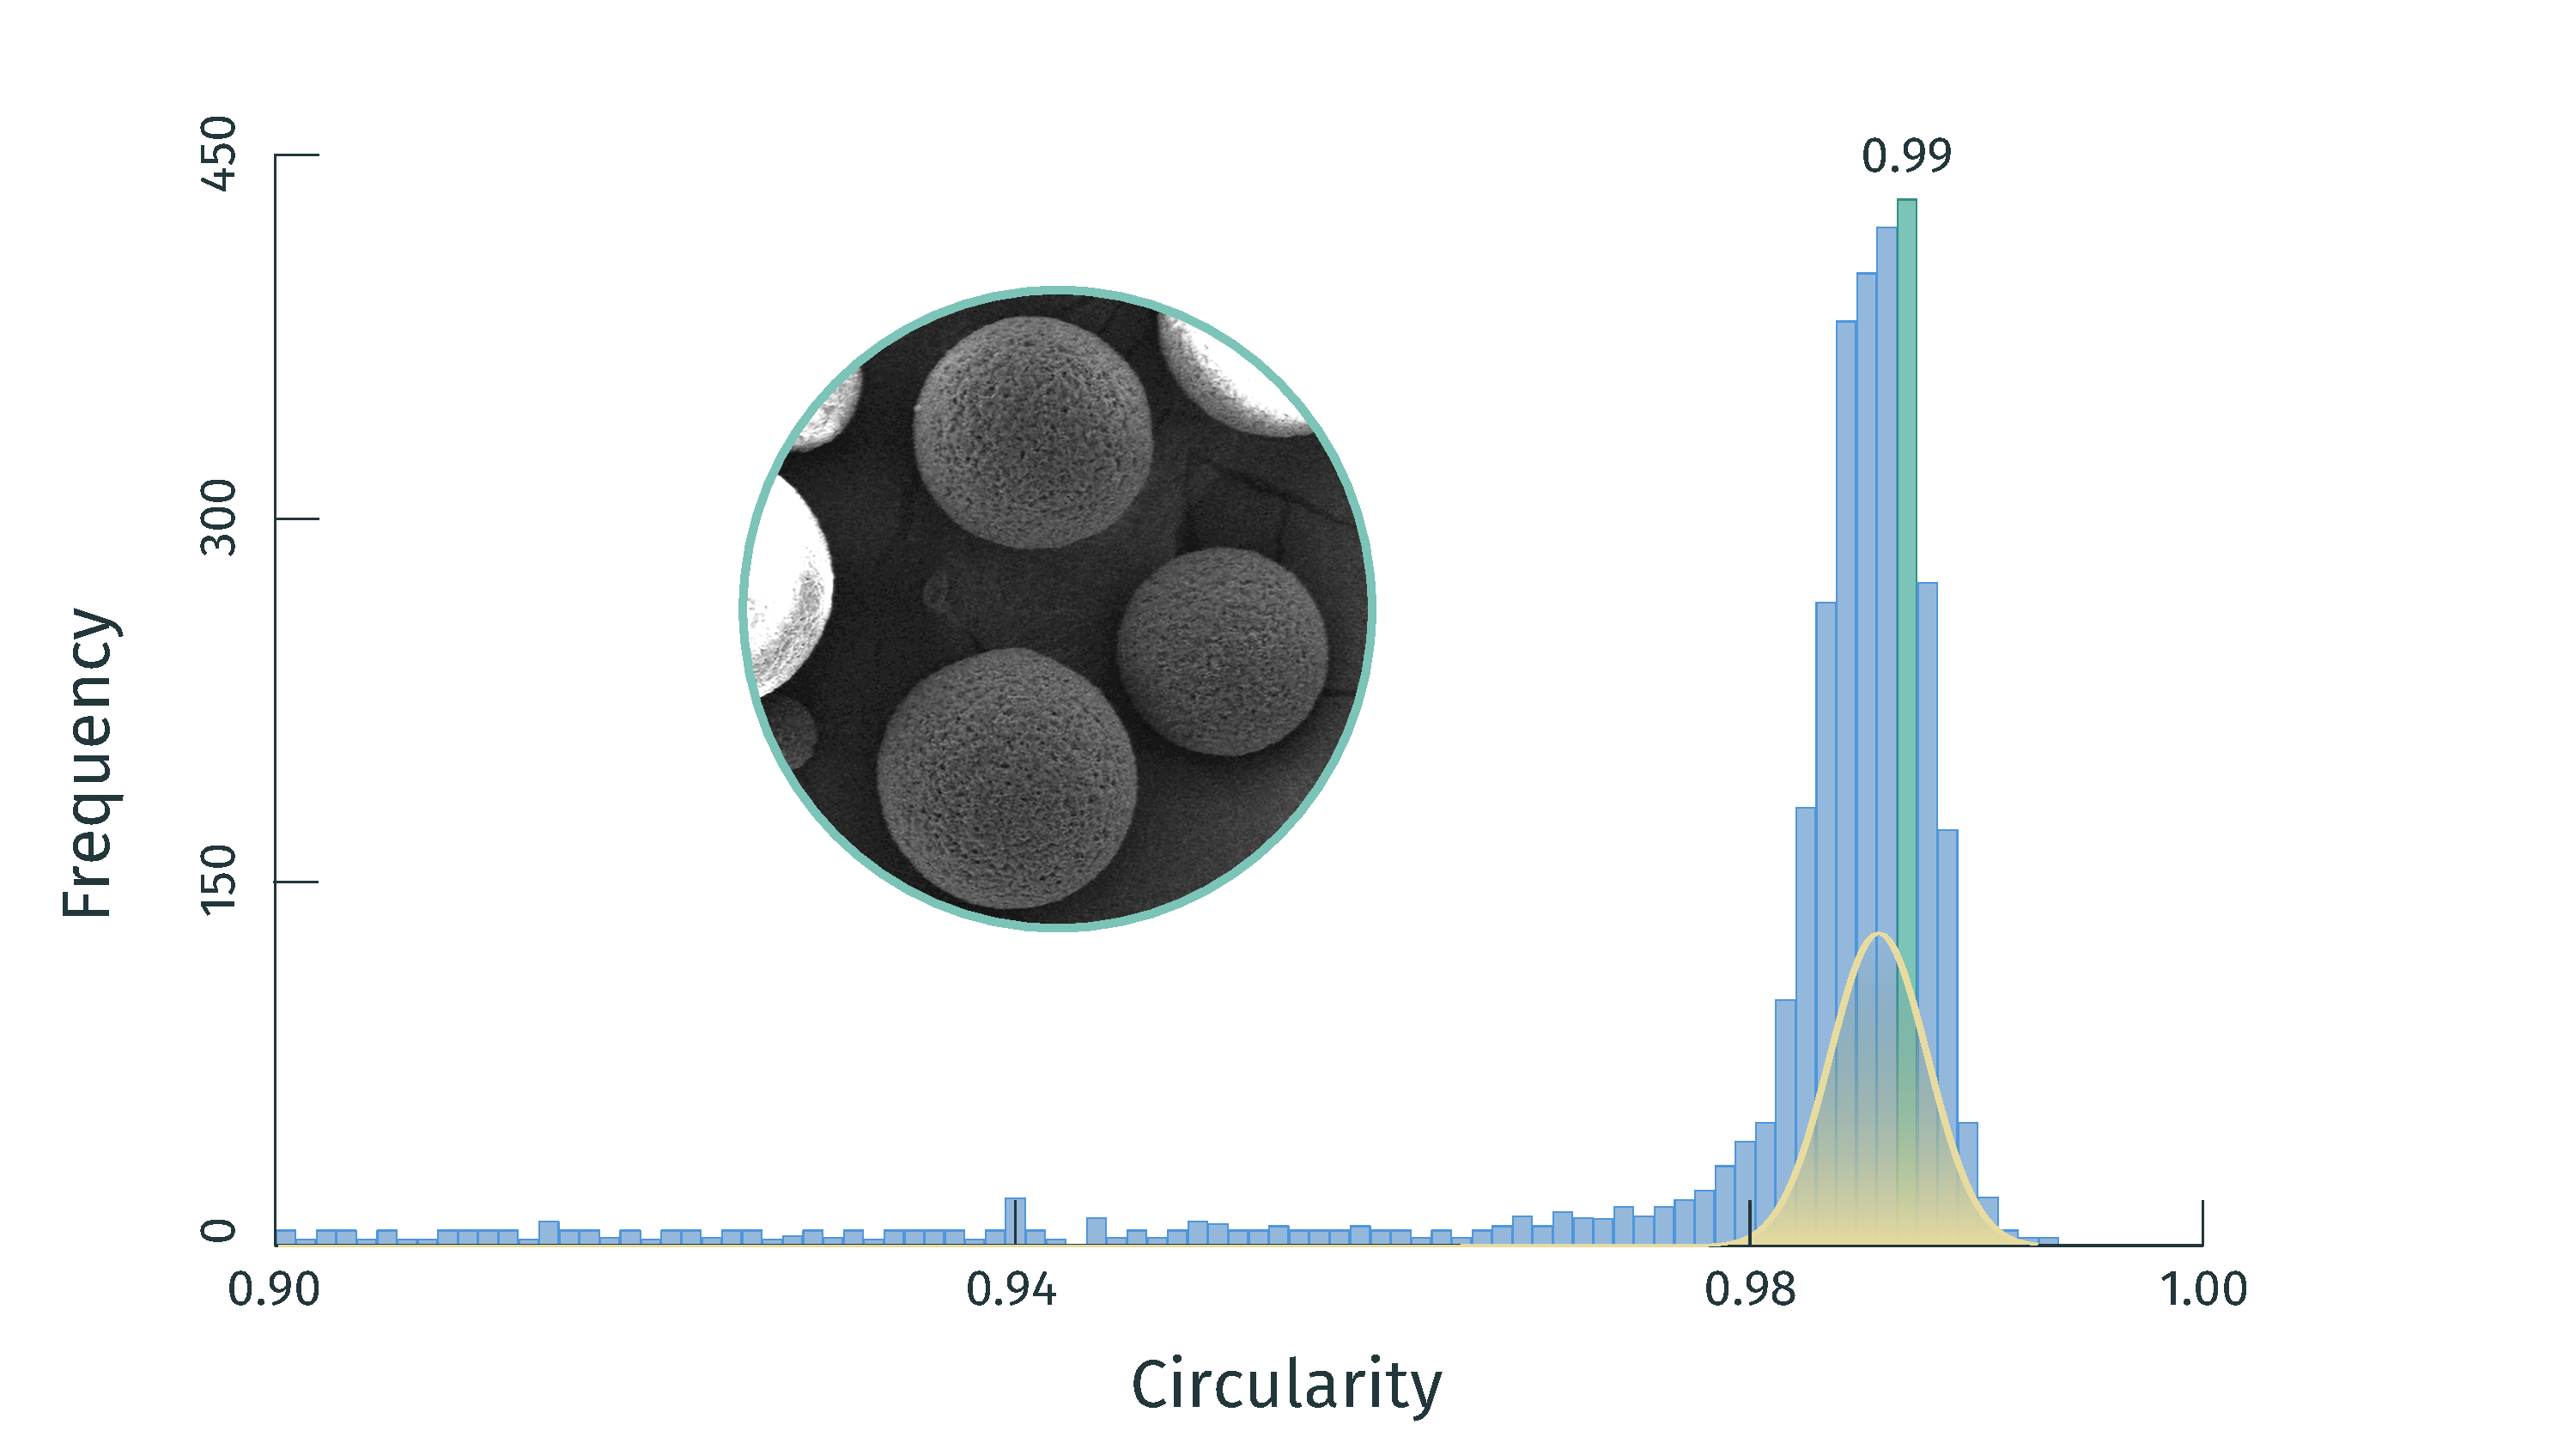
\includegraphics[width=0.8\textwidth]{Pictures/Vector/PDF/PSD_circularity.pdf}
        \end{figure}
      }


    \end{frame}

    \subsection{Stabilità termica}


    \begin{frame}
      \frametitle{Stabilità termica}

      \onslide*<1>{
        \begin{center}
          \alert<1>{Quali sono le caratteristiche termiche della polvere ottenuta?}
        \end{center}
        }
      
      \onslide*<2->{La polvere è stata sottoposta a due analisi fondamentali:}

      \begin{itemize}
        \item <3-> \textbf{Calorimetria Differenziale a Scansione}
        \item <4>  \textbf{Analisi Termogravimetrica}
      \end{itemize}
    
    \end{frame}
      \subsubsection{Calorimetria Differenziale a Scansione}

        \begin{frame}
          \frametitle{Calorimetria Differenziale a Scansione}

          \onslide*<1>{La calorimetria differenziale a scansione (\textbf{DSC}) è un metodo di analisi che permette di studiare la variazione di energia di un campione sottoposto ad un aumento e decremento graduale di temperatura.}
          \onslide*<2->{
            \begin{center}
              Cosa permette di individuare nei \textbf{polimeri}?
            \end{center}
          }
            \begin{itemize}
              \item <3-> \textbf{Temperature di fusione}
              \item <4-> \textbf{Temperature di cristallizzazione}
              \item <5-> \textbf{Finestra di sinterizzazione}
            \end{itemize}
        
        \end{frame}

        \begin{frame}
          \frametitle{DSC}
        
          \onslide*<1>{La prova è stata svolta in \textit{aria} in un intervallo di temperatura da \textit{-50 a 180 $ ^{\circ}C$}, su campioni di \textbf{polvere} e \textbf{pellet}, con una rampa 
          di riscaldamento di \textit{10 $ ^{\circ}C$/min}}

          \onslide*<2>{
            \begin{figure}[h]
              \centering
              \caption{DSC of a pellet and a powder sample}
              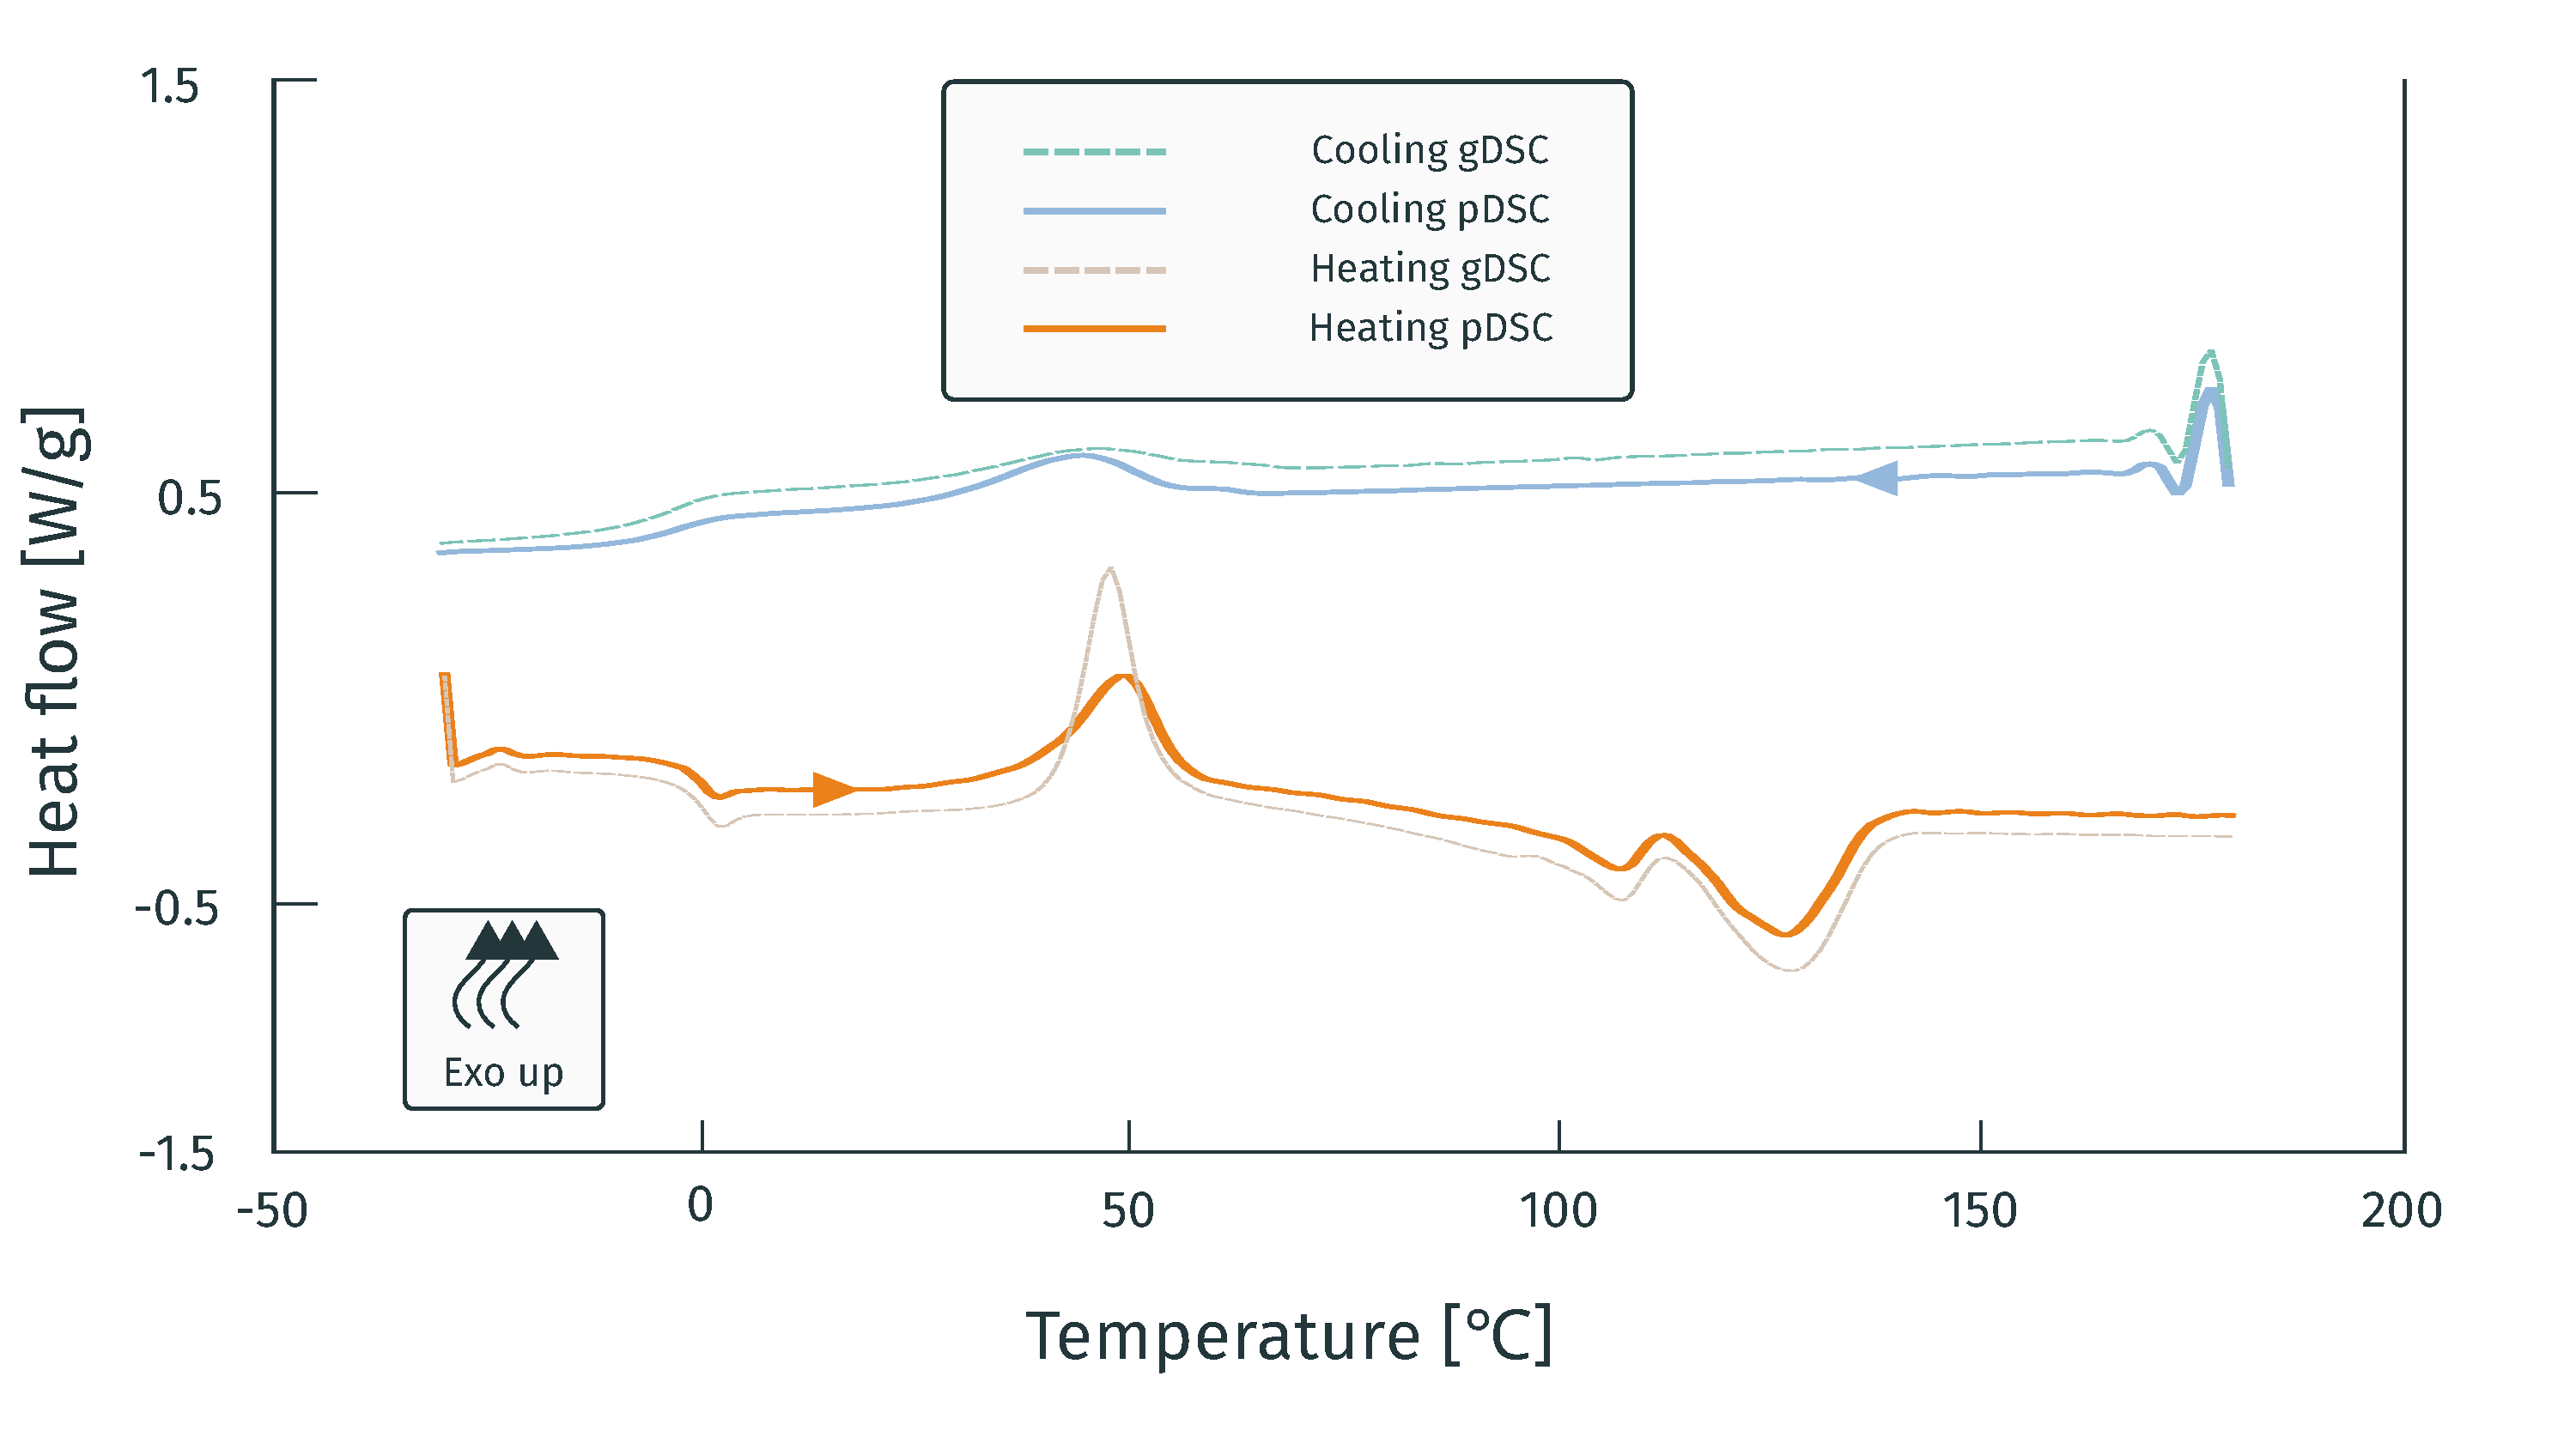
\includegraphics[width=0.8\textwidth]{Pictures/Vector/PDF/DSC/DSC.pdf}
            \end{figure}
          }

          \onslide*<3>{
            \begin{figure}[h]
              \centering
              \caption{Heating phase}
              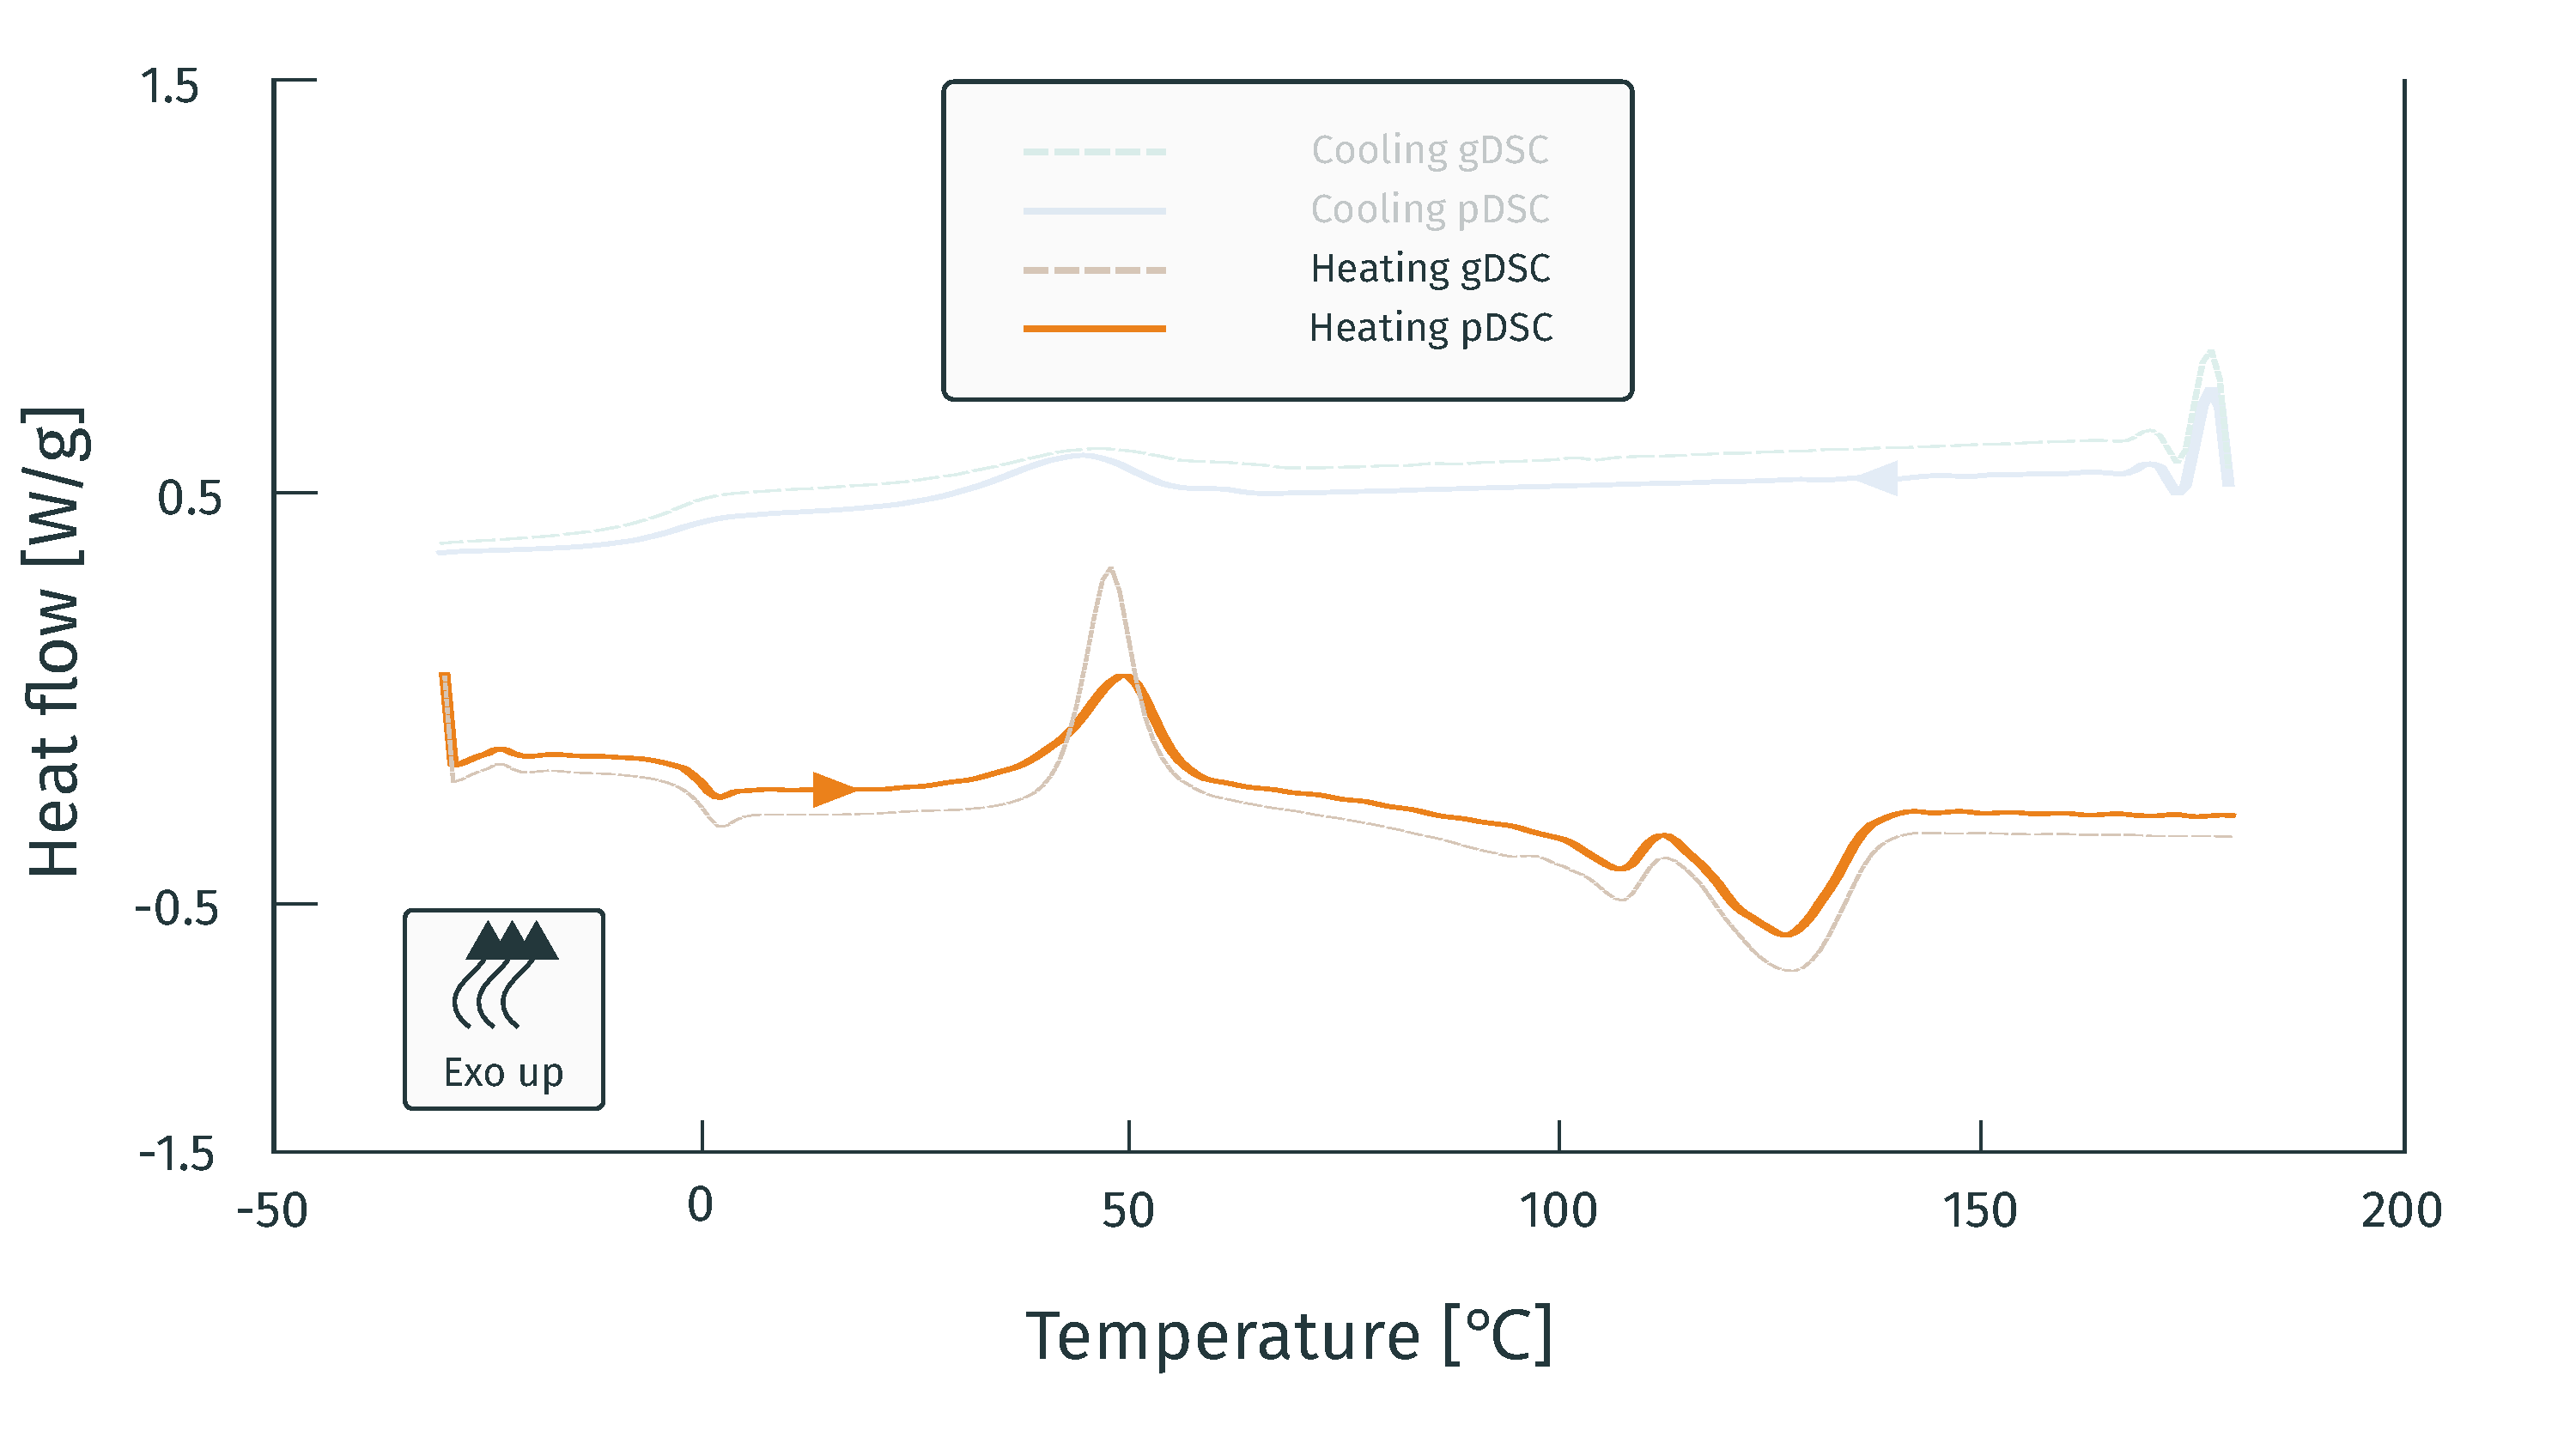
\includegraphics[width=0.8\textwidth]{Pictures/Vector/PDF/DSC/DSC_heating.pdf}
            \end{figure}
          }

          \onslide*<4>{
            \begin{figure}[h]
              \centering
              \caption{Cooling phase} 
              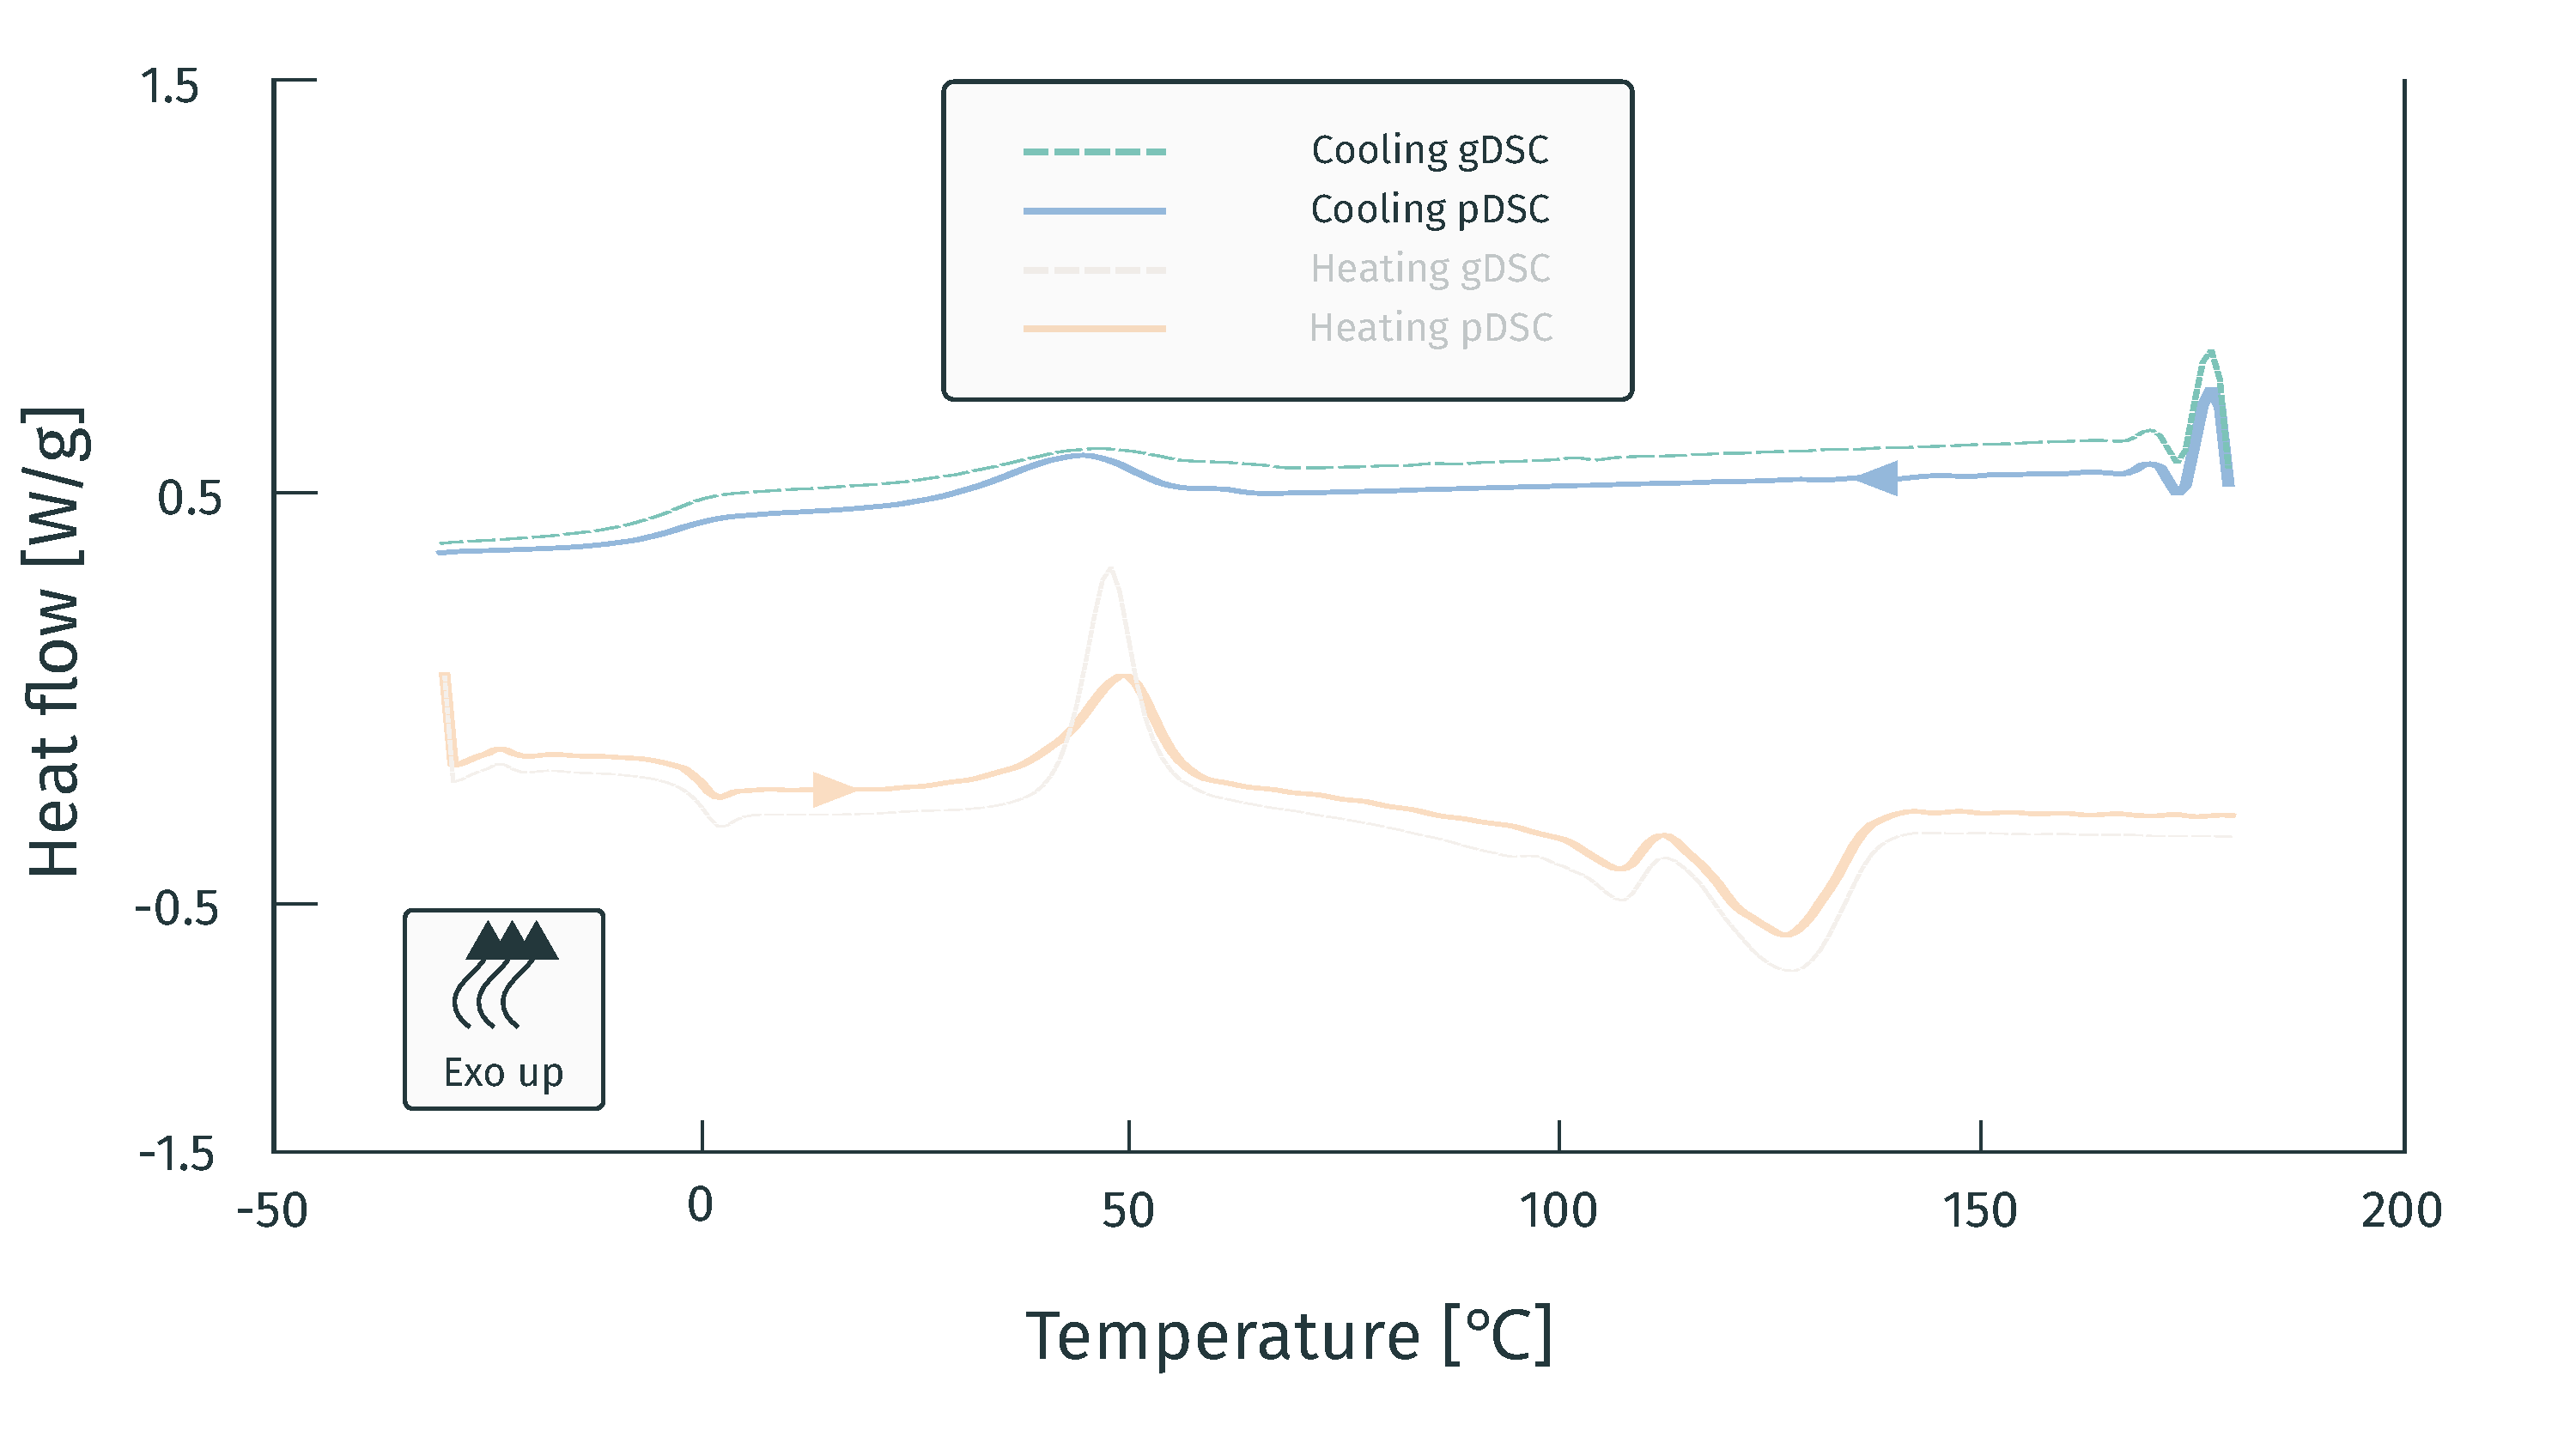
\includegraphics[width=0.8\textwidth]{Pictures/Vector/PDF/DSC/DSC_cooling.pdf}
            \end{figure}
          }

          \onslide*<5>{

            \begin{figure}[h]
              \centering
              \caption{Cold crystallyzation}
              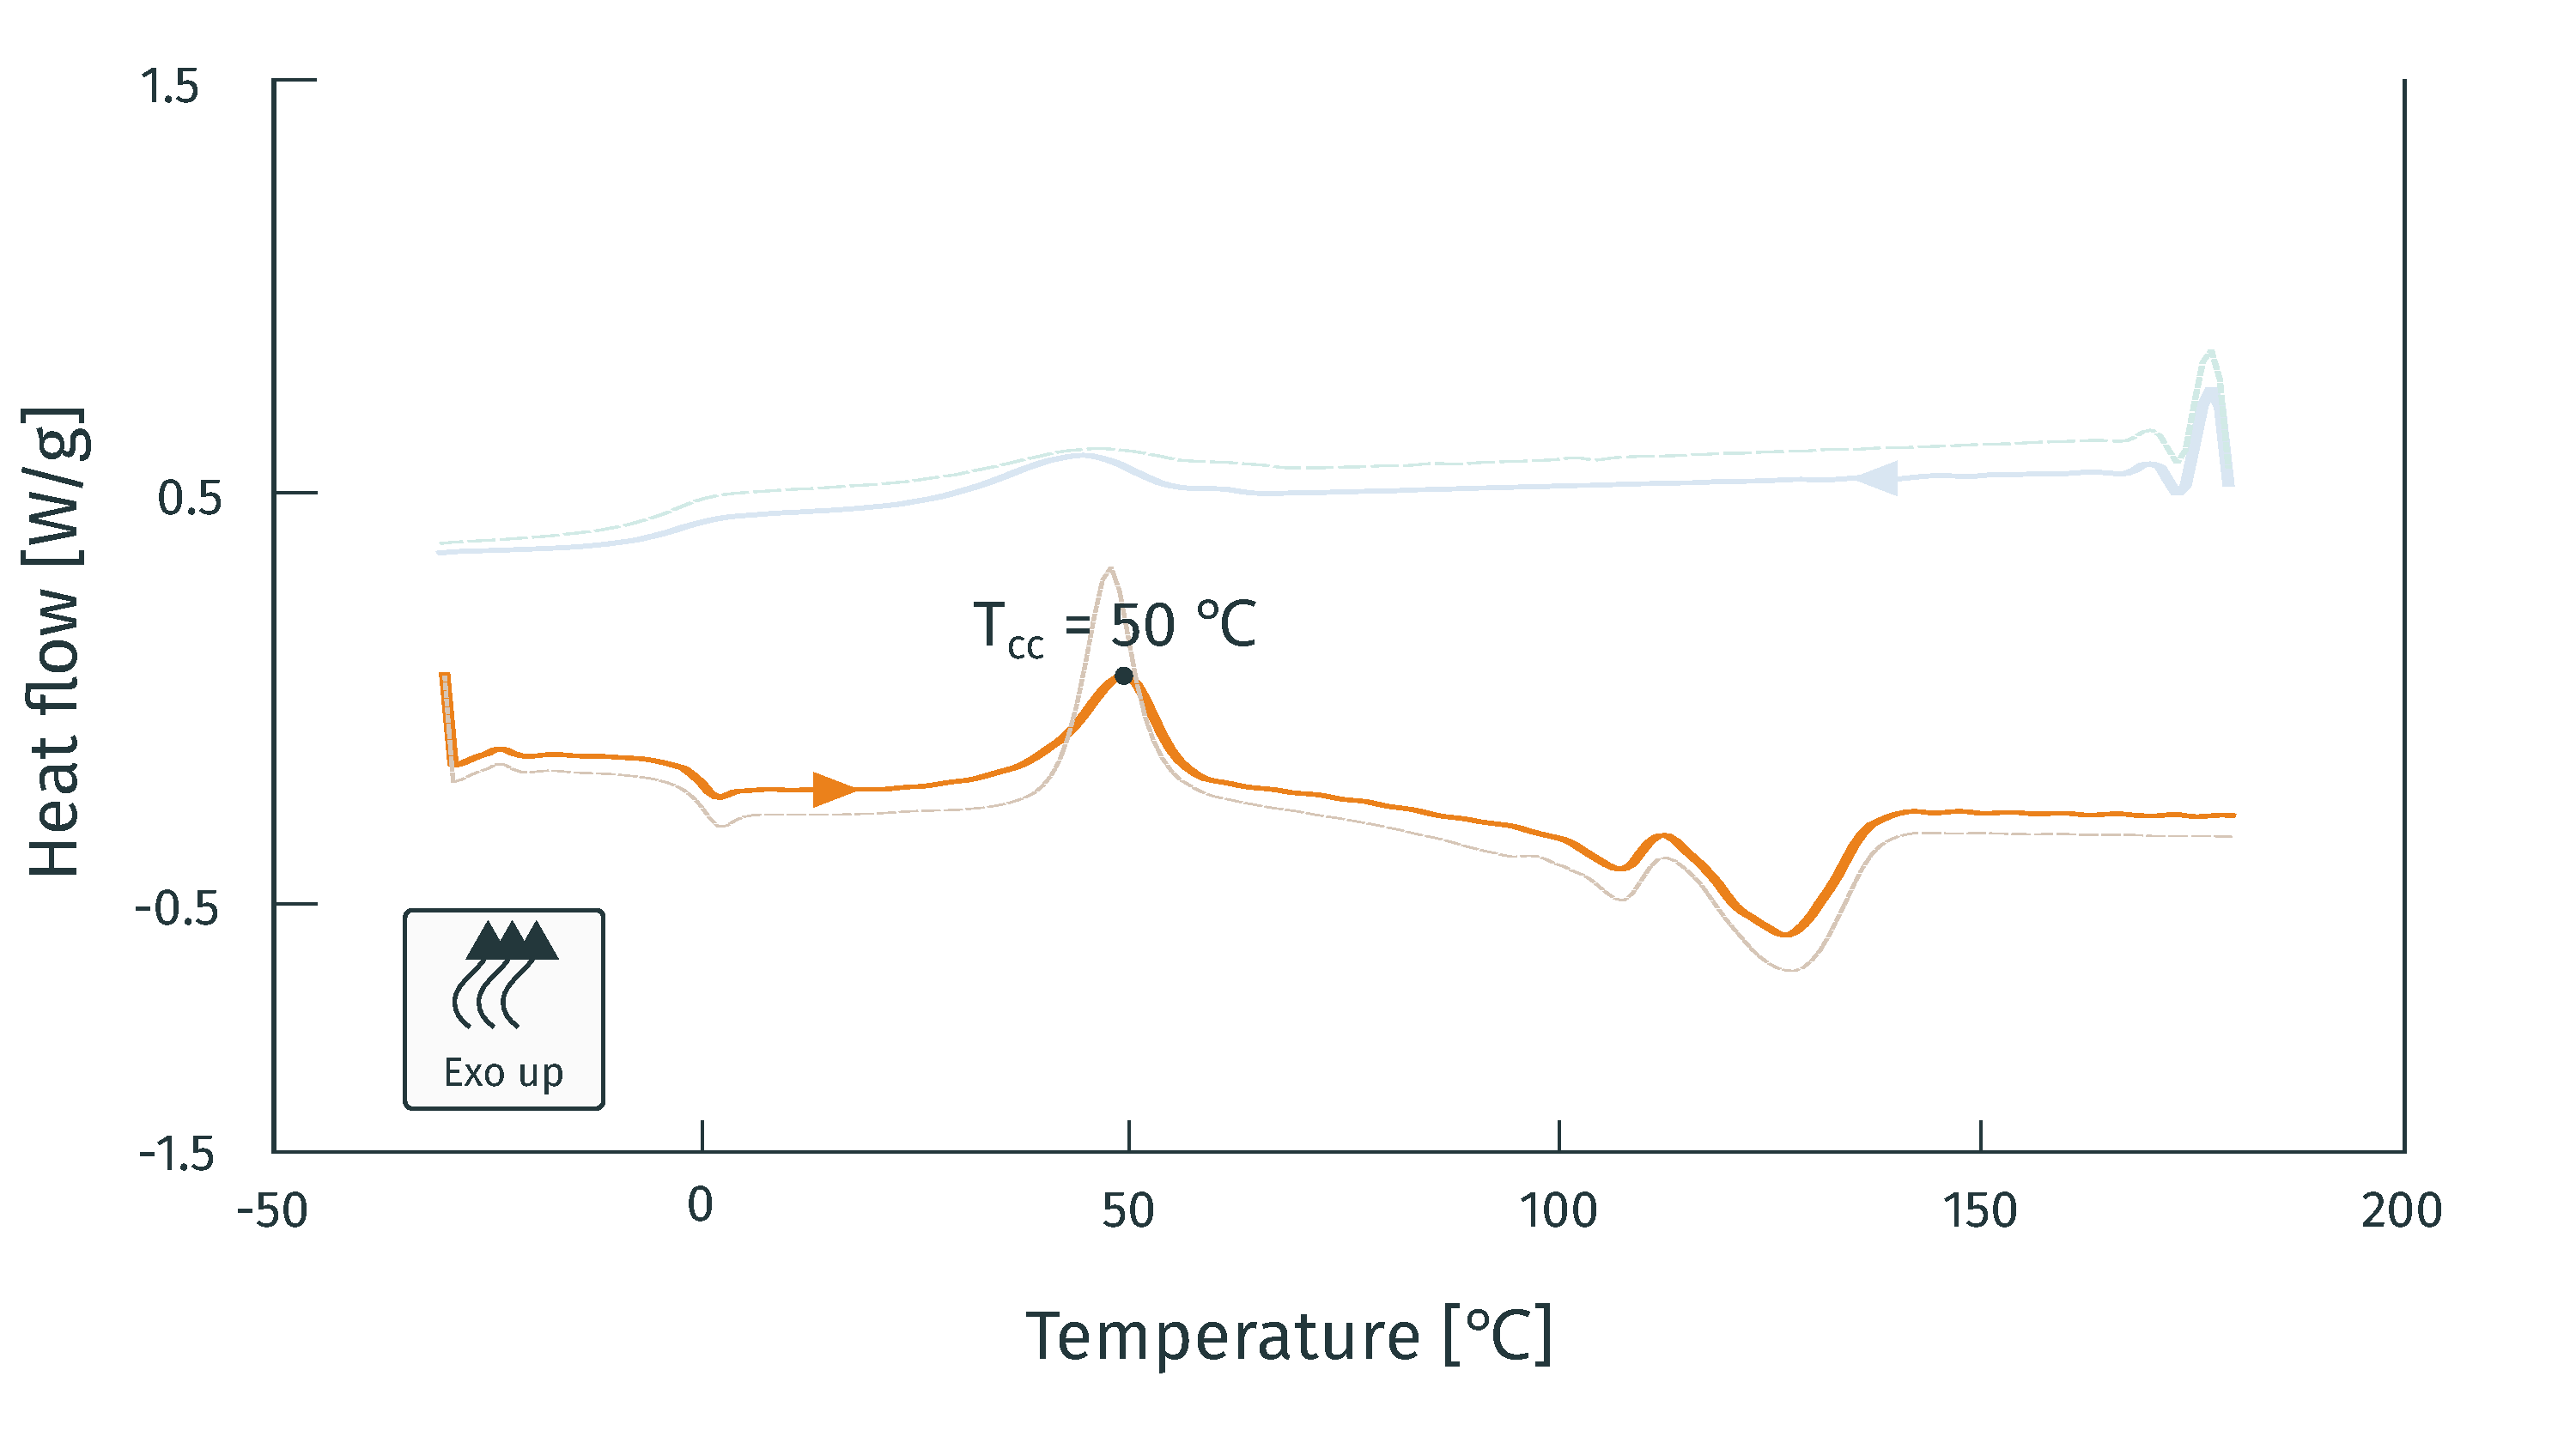
\includegraphics[width=0.8\textwidth]{Pictures/Vector/PDF/DSC/DSC_points-1.pdf}
            \end{figure}
          }

          \onslide*<6>{

            \begin{figure}[h]
              \centering
              \caption{Melting points}
              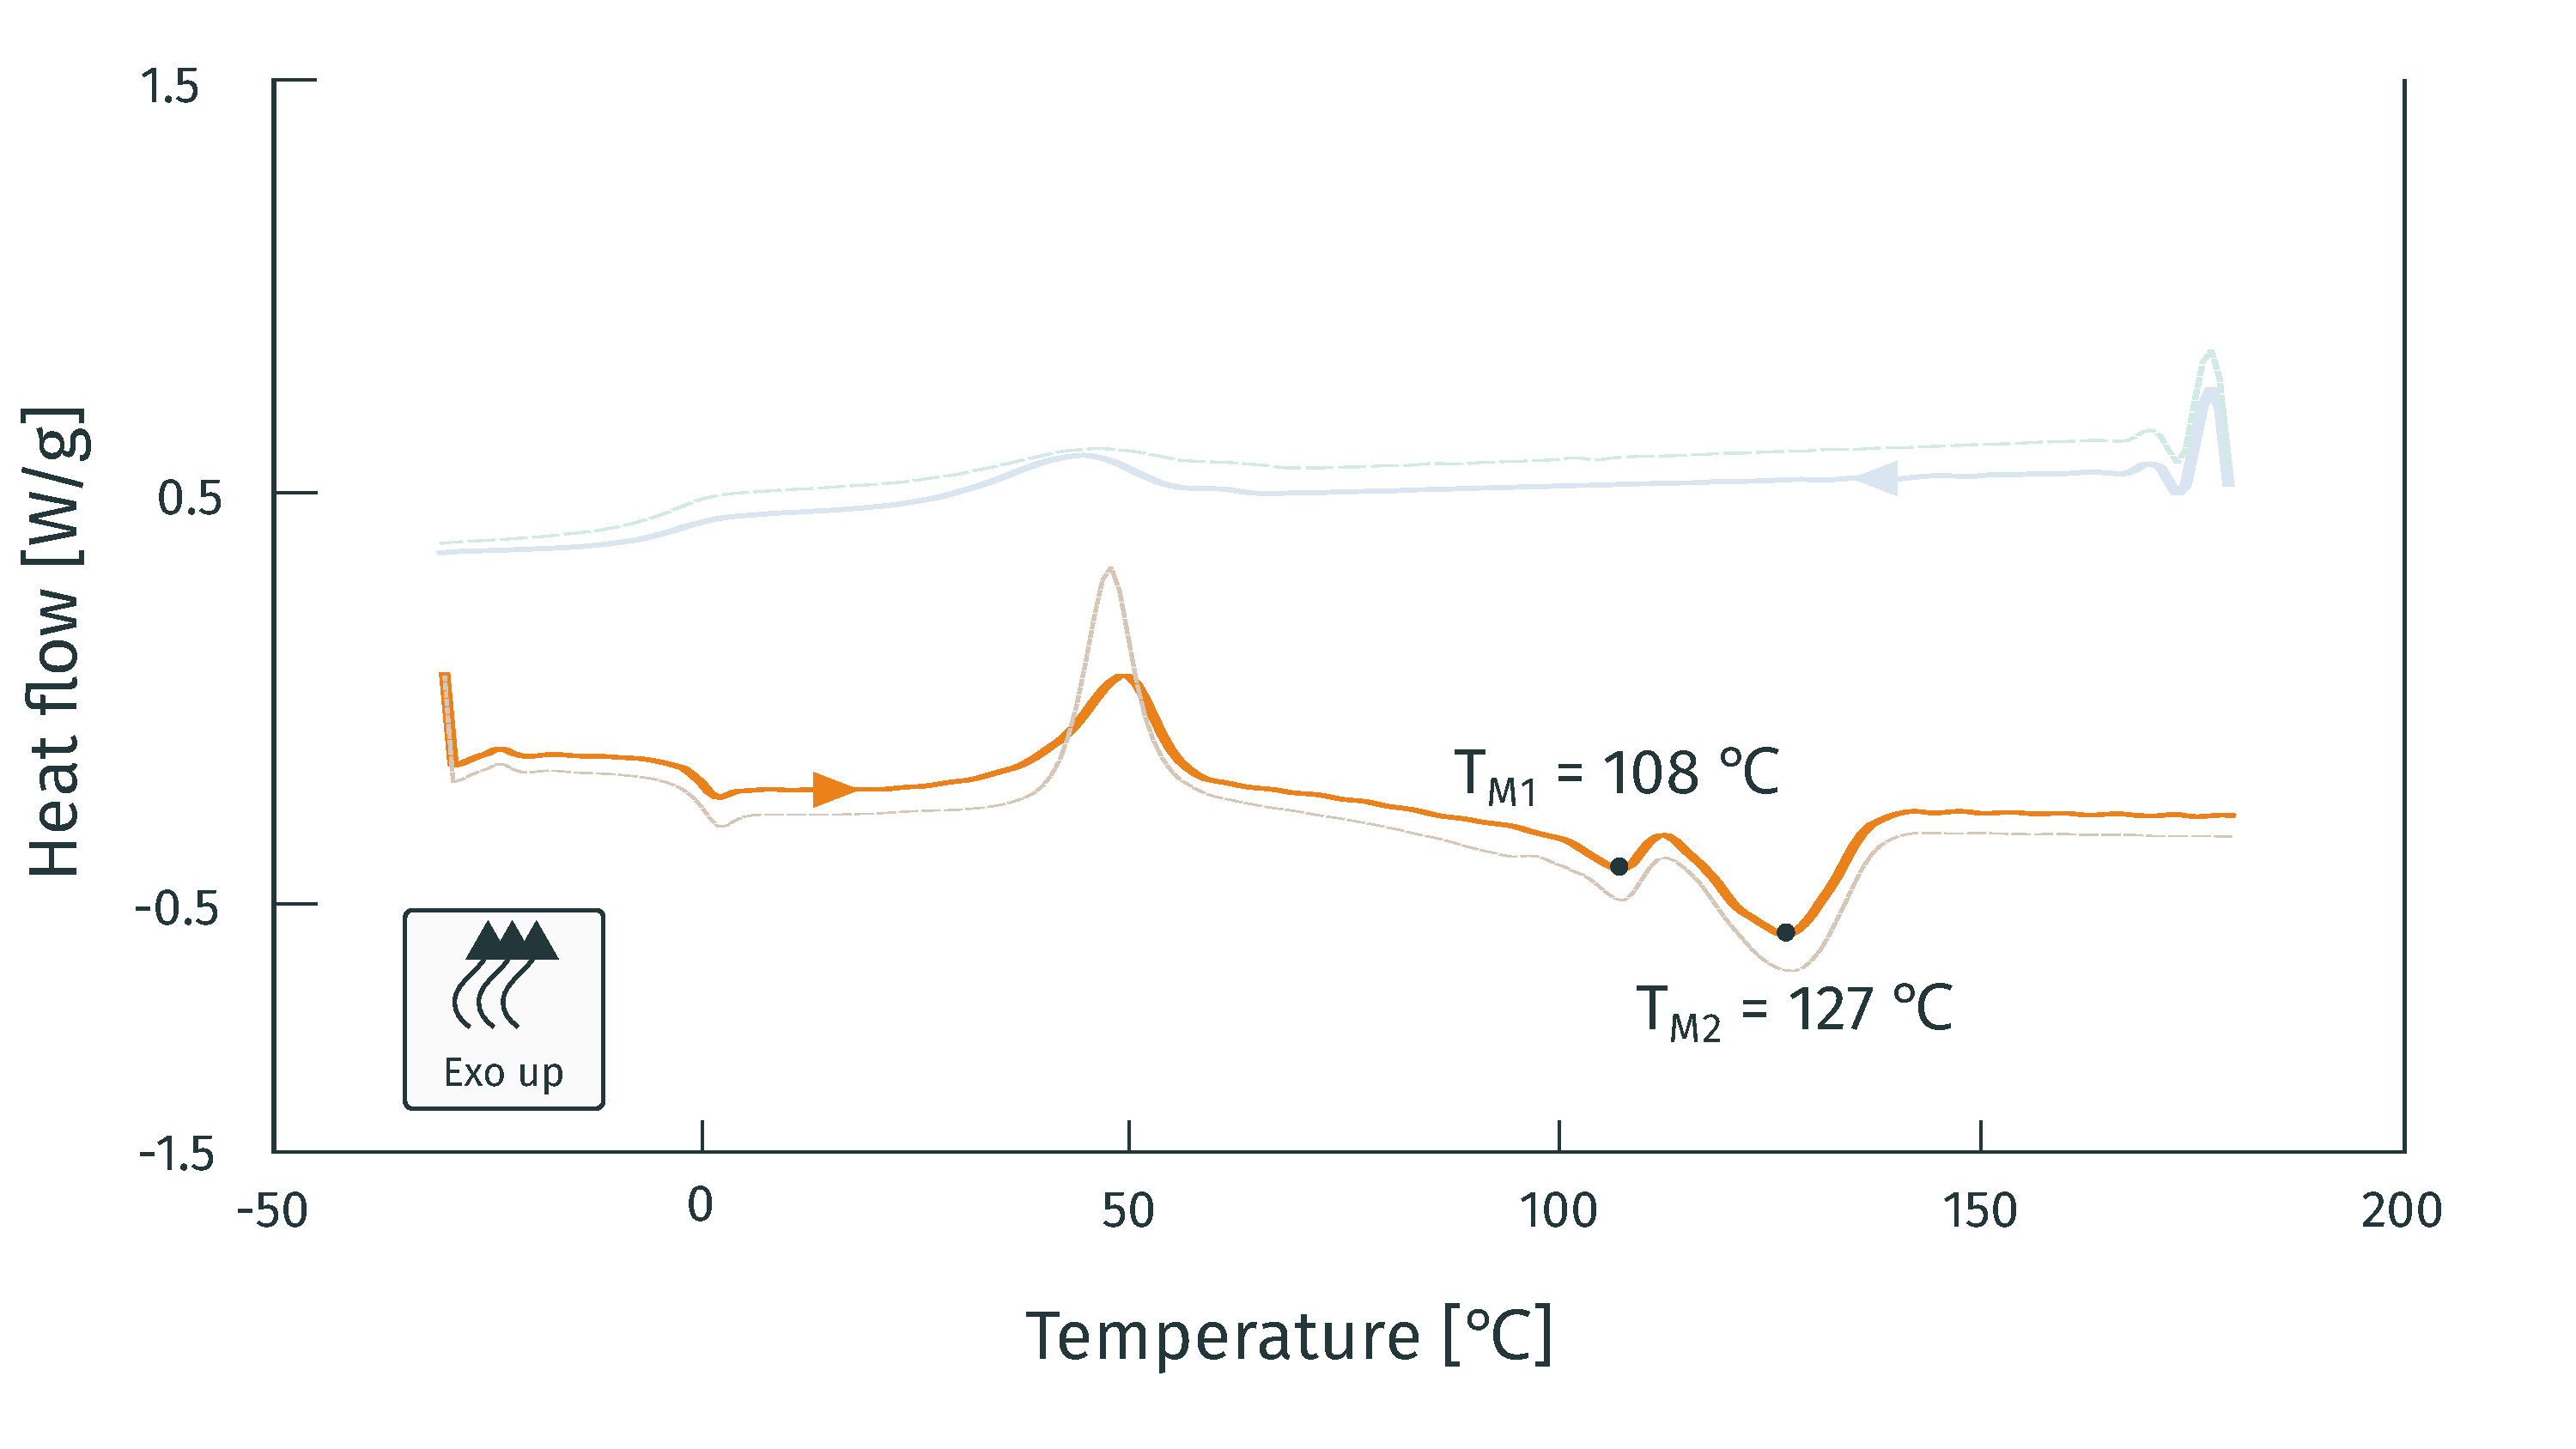
\includegraphics[width=0.8\textwidth]{Pictures/Vector/PDF/DSC/DSC_points-2.pdf}
            \end{figure}
          }

          \onslide*<7>{

            \begin{figure}[h]
              \centering
              \caption{Sintering window}
              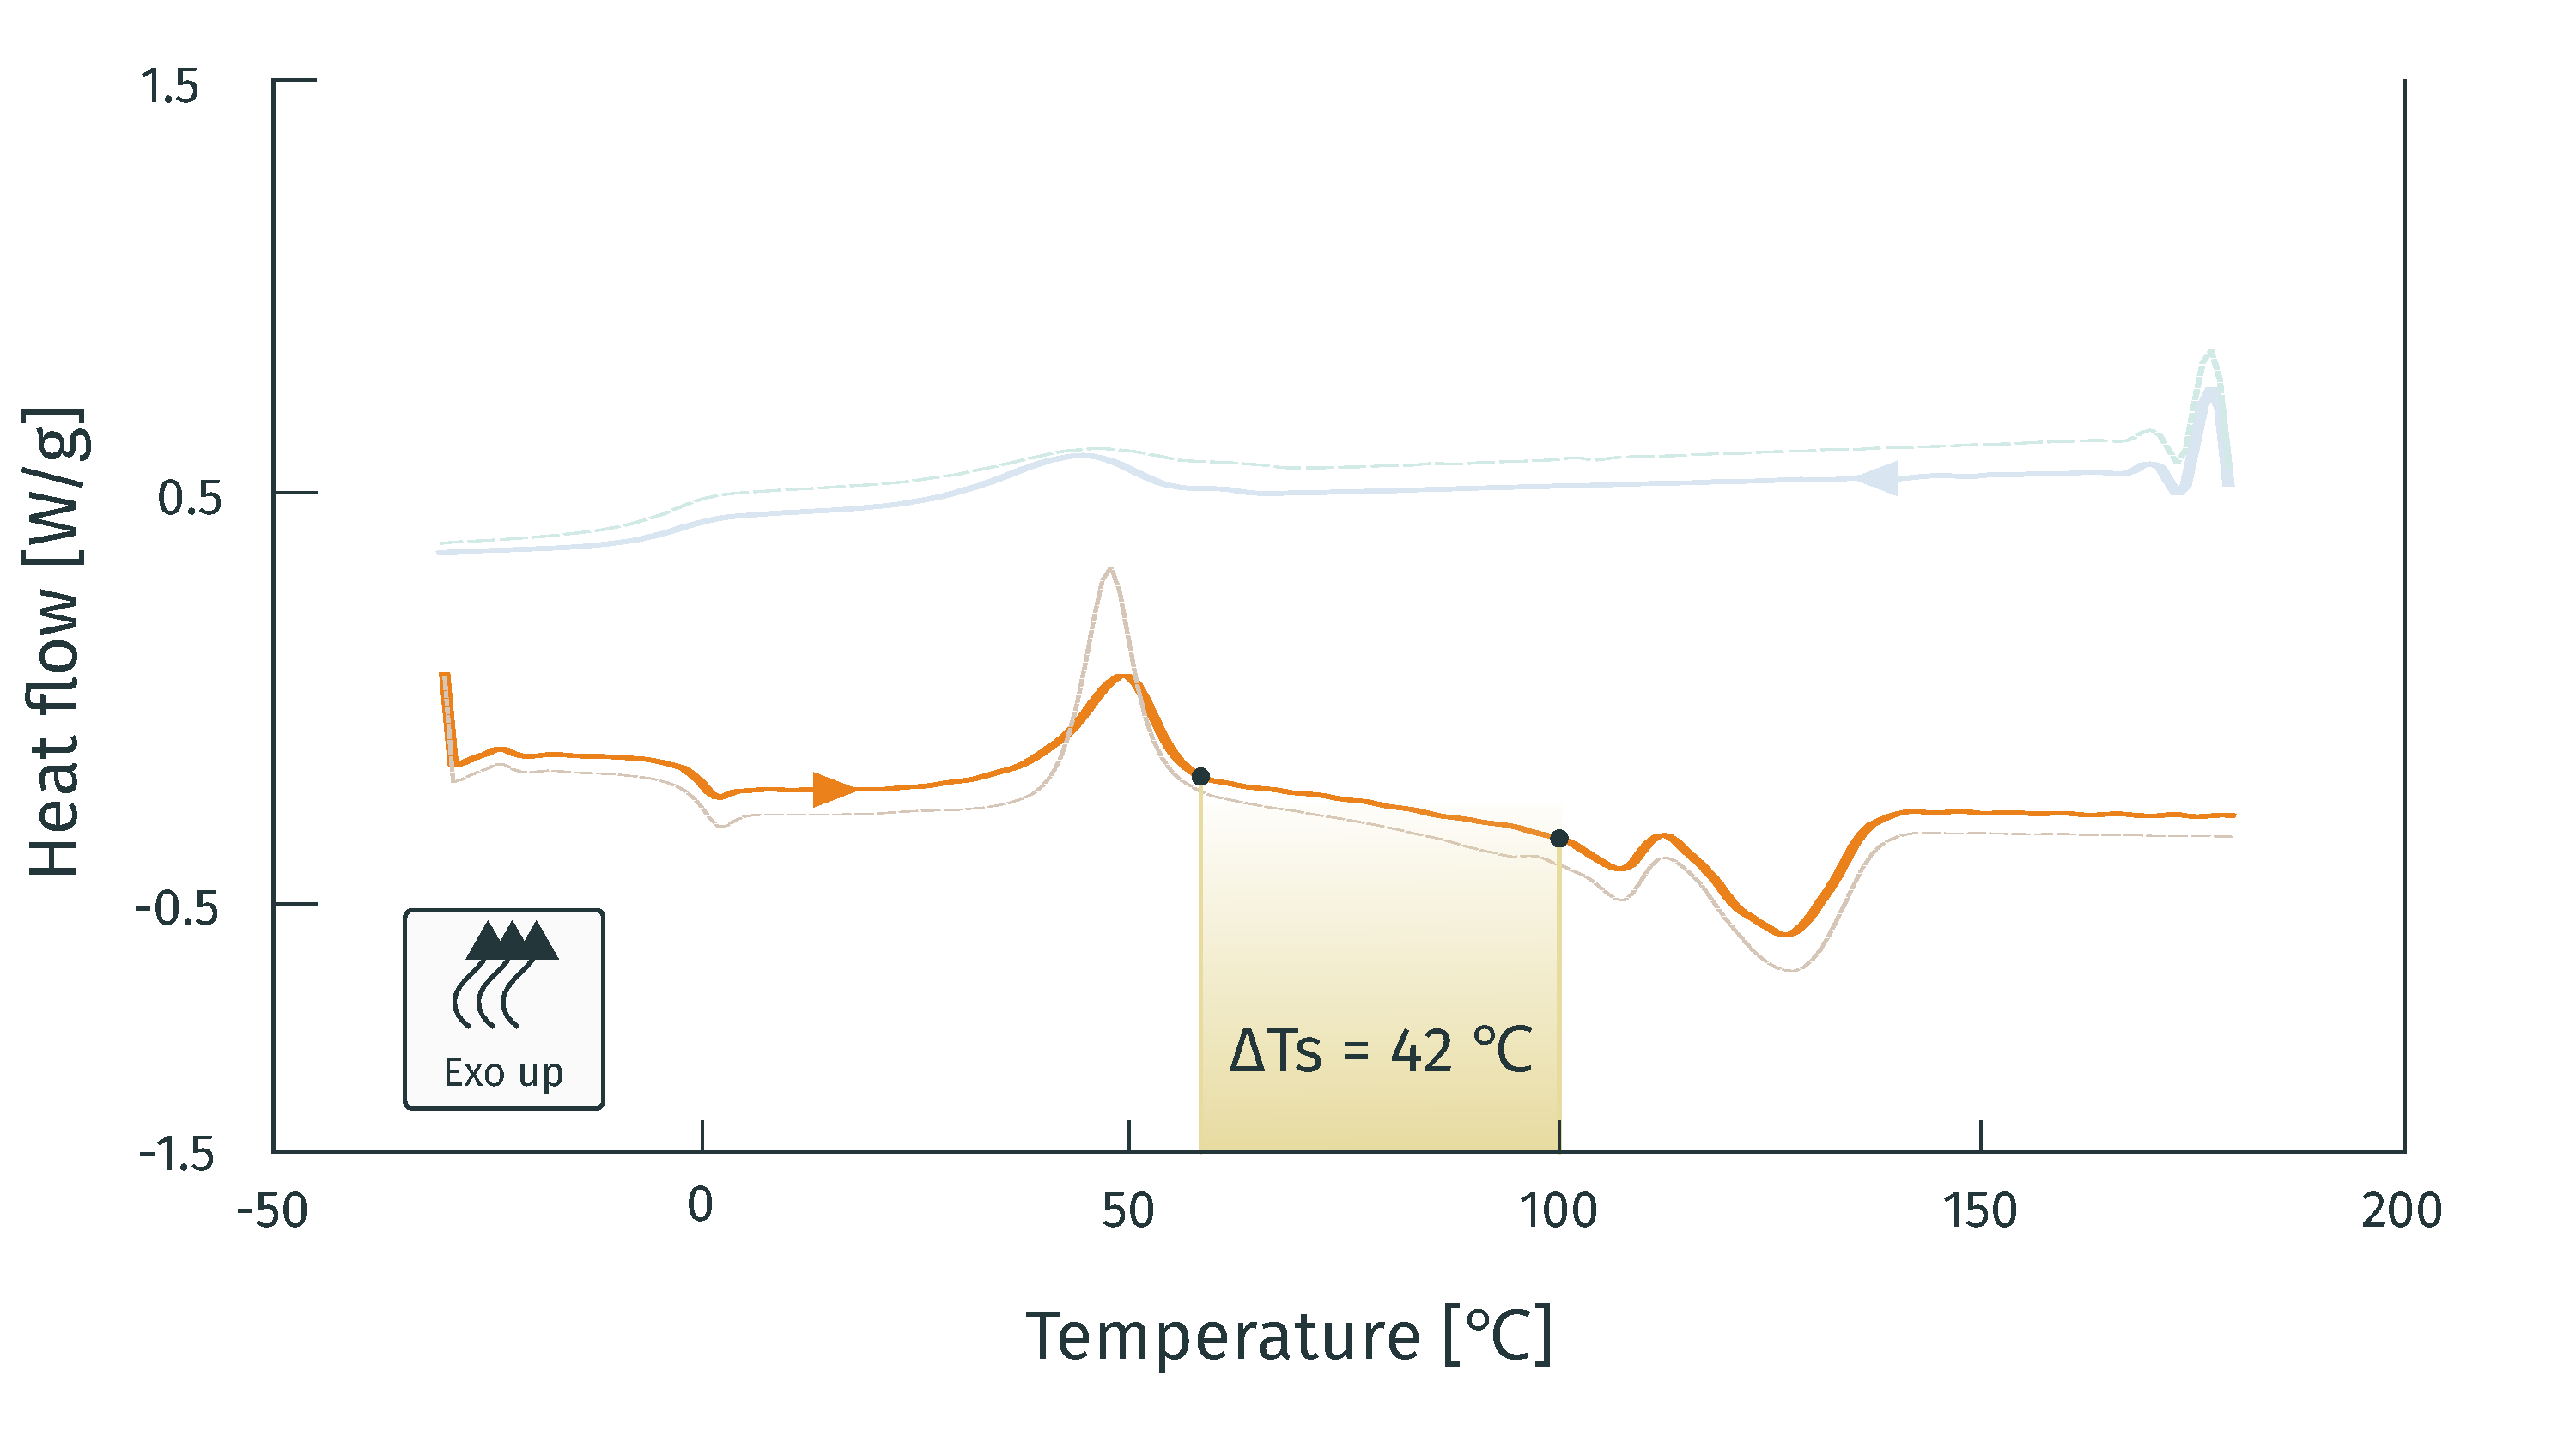
\includegraphics[width=0.8\textwidth]{Pictures/Vector/PDF/DSC/DSC_points-3.pdf}
            \end{figure}
          }

          \onslide*<8>{

            \begin{figure}[h]
              \centering
              \caption{Crystallization}
              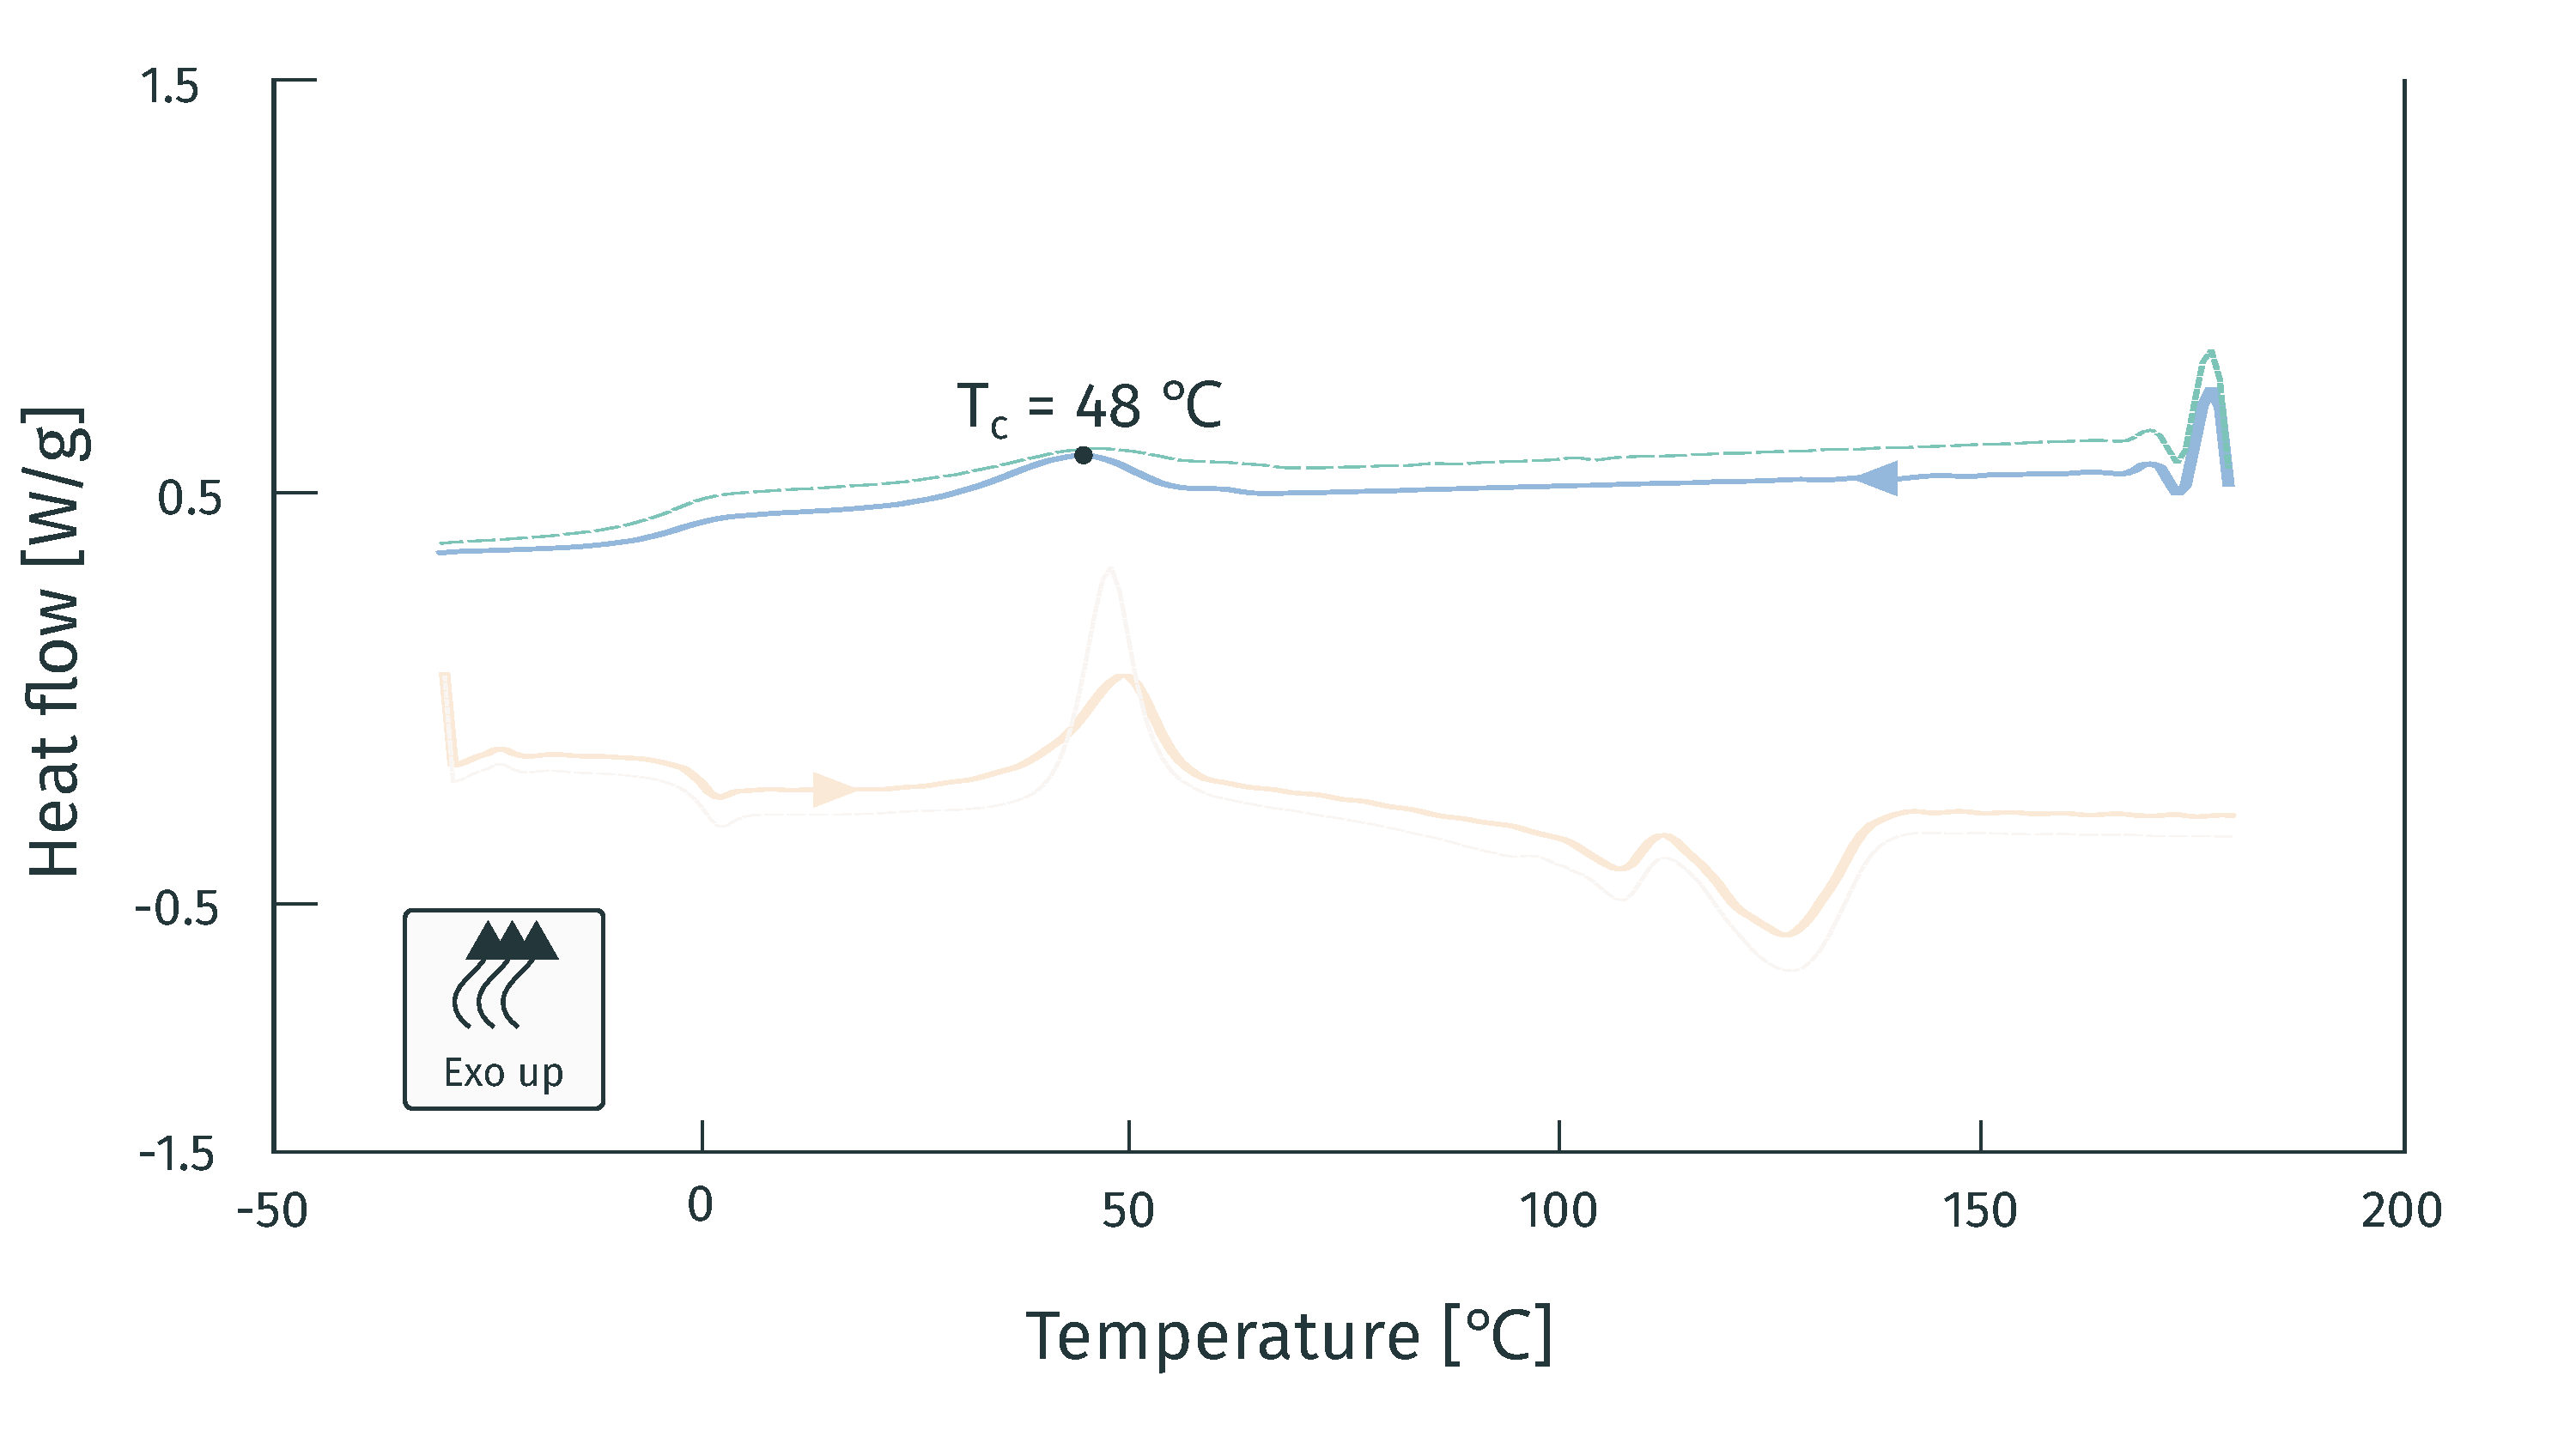
\includegraphics[width=0.8\textwidth]{Pictures/Vector/PDF/DSC/DSC_points-4.pdf}
            \end{figure}
          }
        
        \end{frame}
      \subsubsection{Analisi termogravimetrica}

        \begin{frame}
          \frametitle{Analisi termogravimetrica}

          \onslide*<1>{L'analisi termogravimetrica (\textbf{TGA}) permette di studiare la degradazione di un campione sottoposto ad un aumento graduale di temperatura.}
          \onslide*<2>{Campioni di \textbf{pellet} e \textbf{polvere} di PHBH sono stati analizzati per verificare che il processo di precipitazione non alterasse il materiale.}
          \onslide*<3>{La prova è stata svolta in \textit{aria} con una rampa di riscaldamento da \textit{25 a 900 $ ^{\circ}C$}, con \textbf{massa normalizzata} su quella iniziale del campione.}

          \onslide*<4>{
            \begin{figure}[h]
              \centering
              \caption{TGA pellet}
              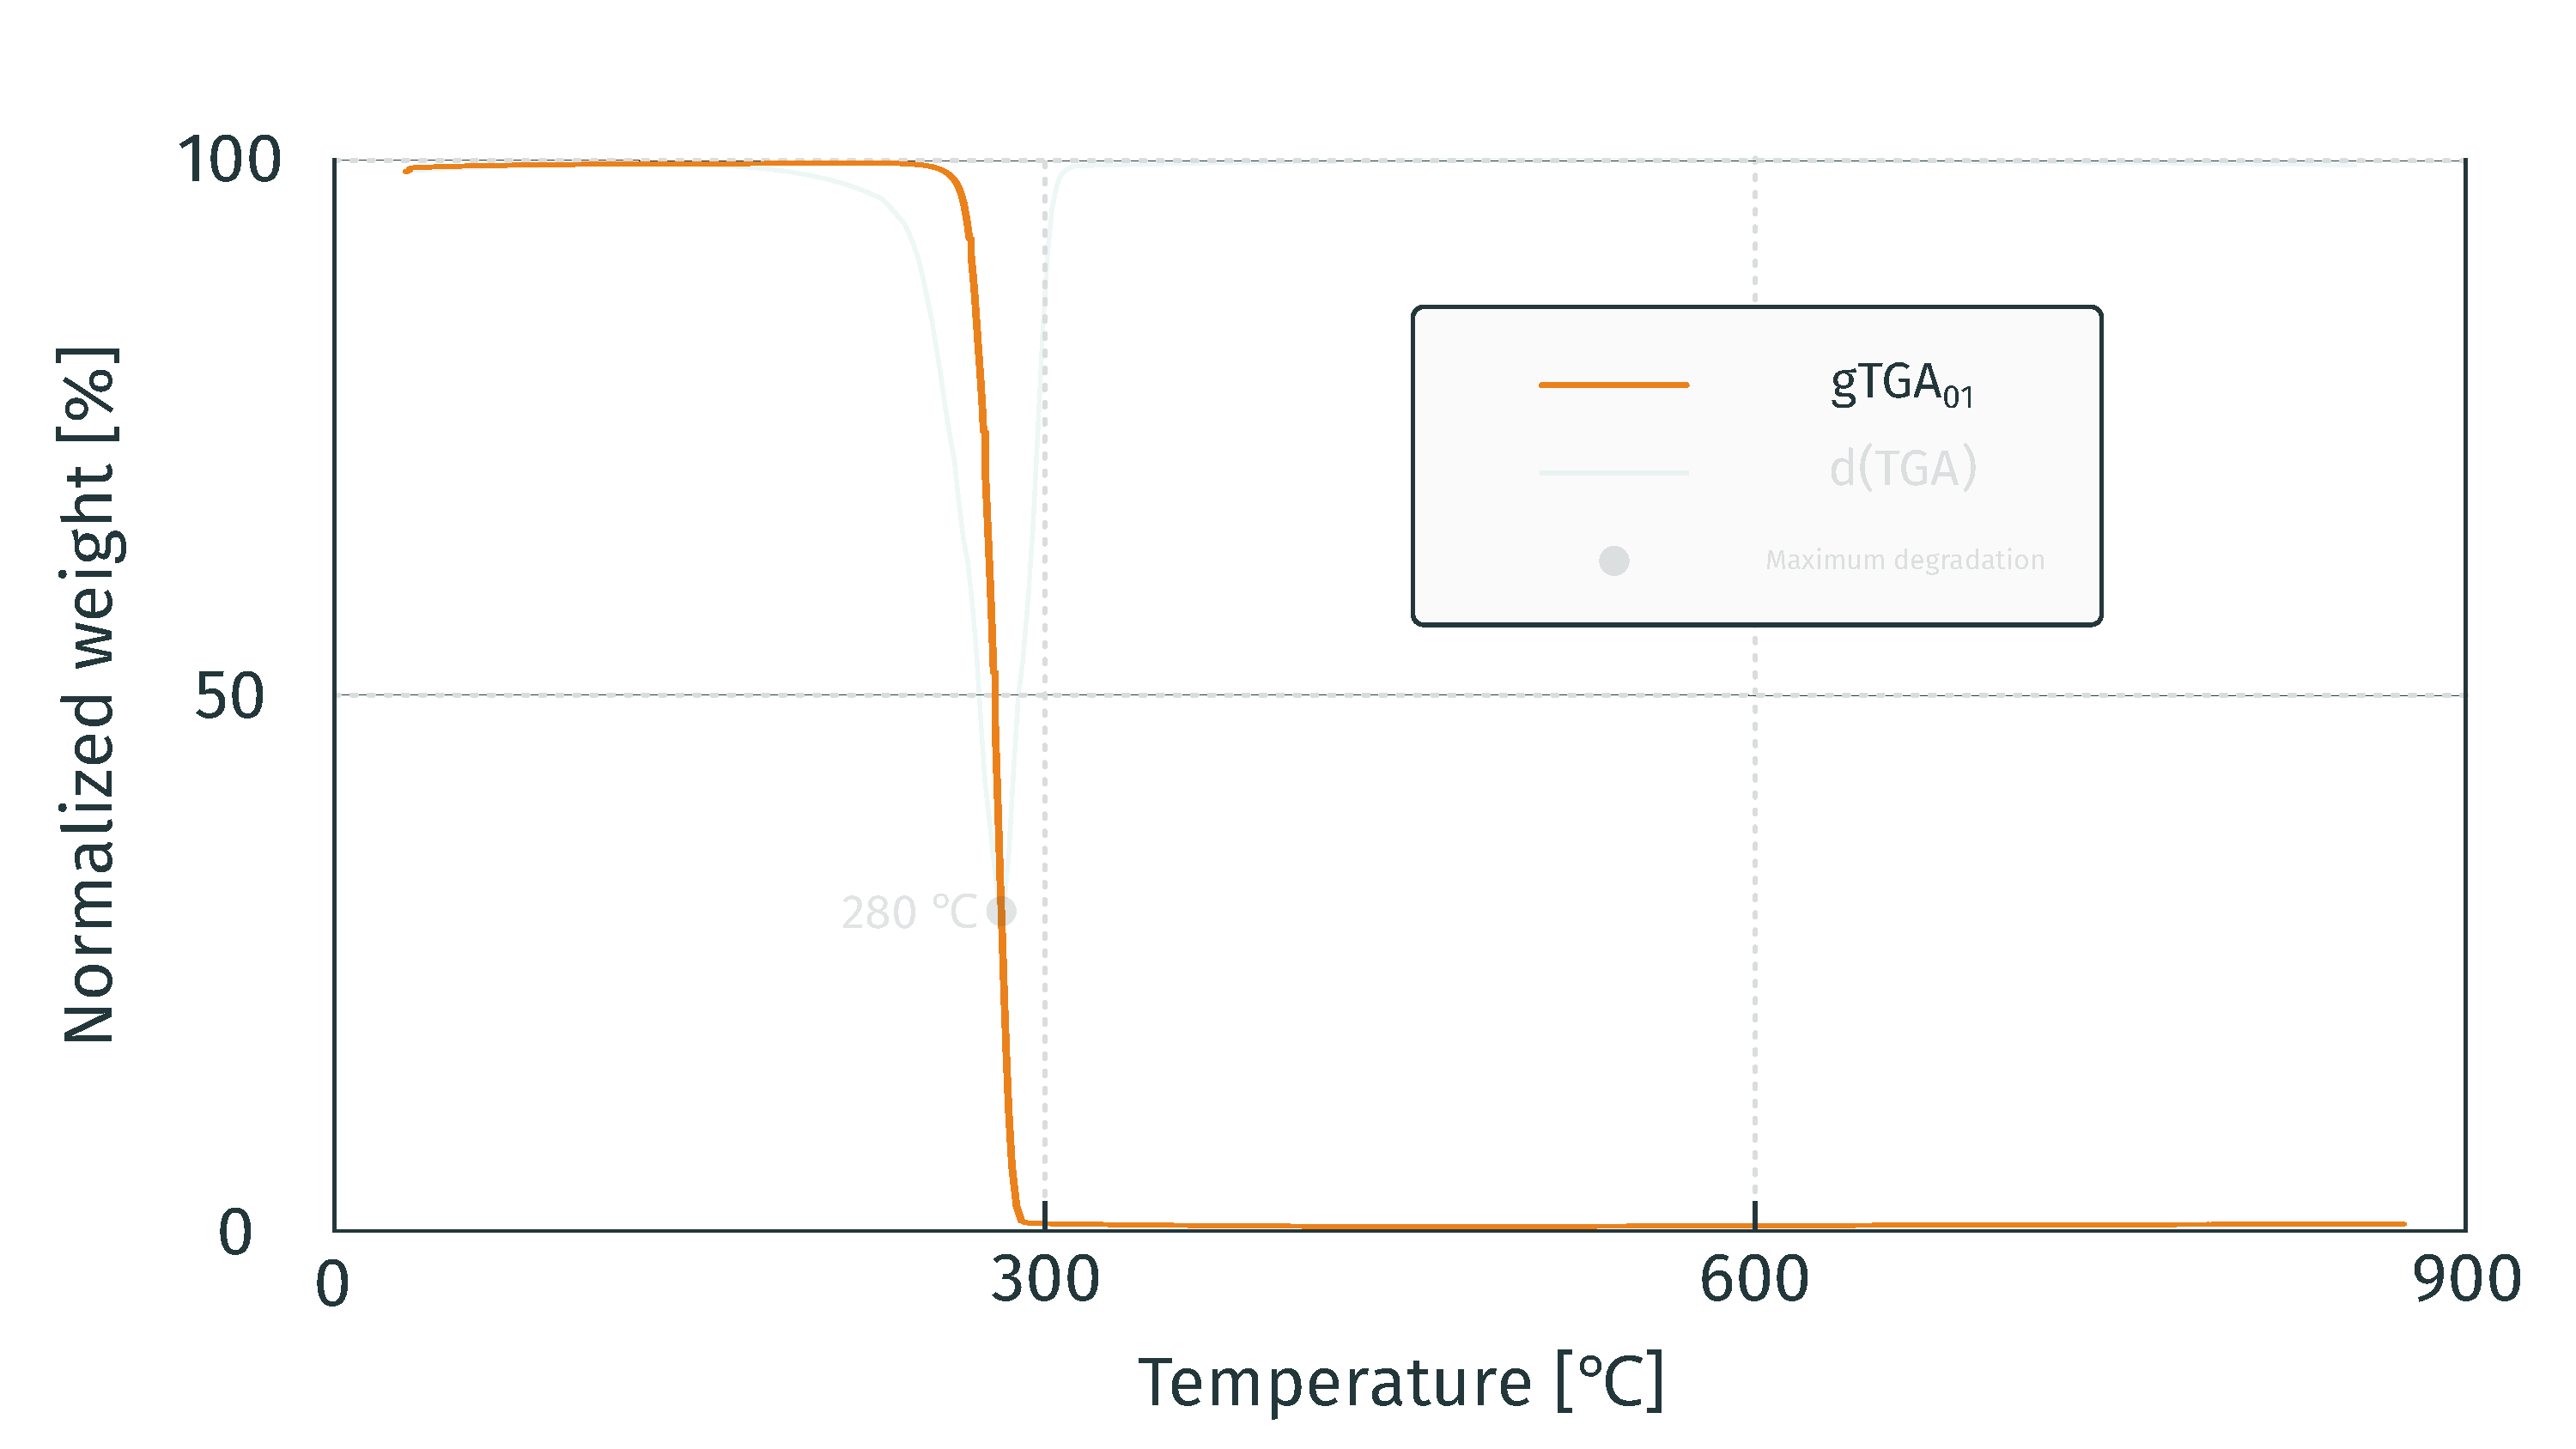
\includegraphics[width=0.8\textwidth]{Pictures/Vector/PDF/TGA/gTGA_noderivative.pdf}
            \end{figure}
          }

          \onslide*<5>{
            \begin{figure}[h]
              \centering
              \caption{TGA pellet}
              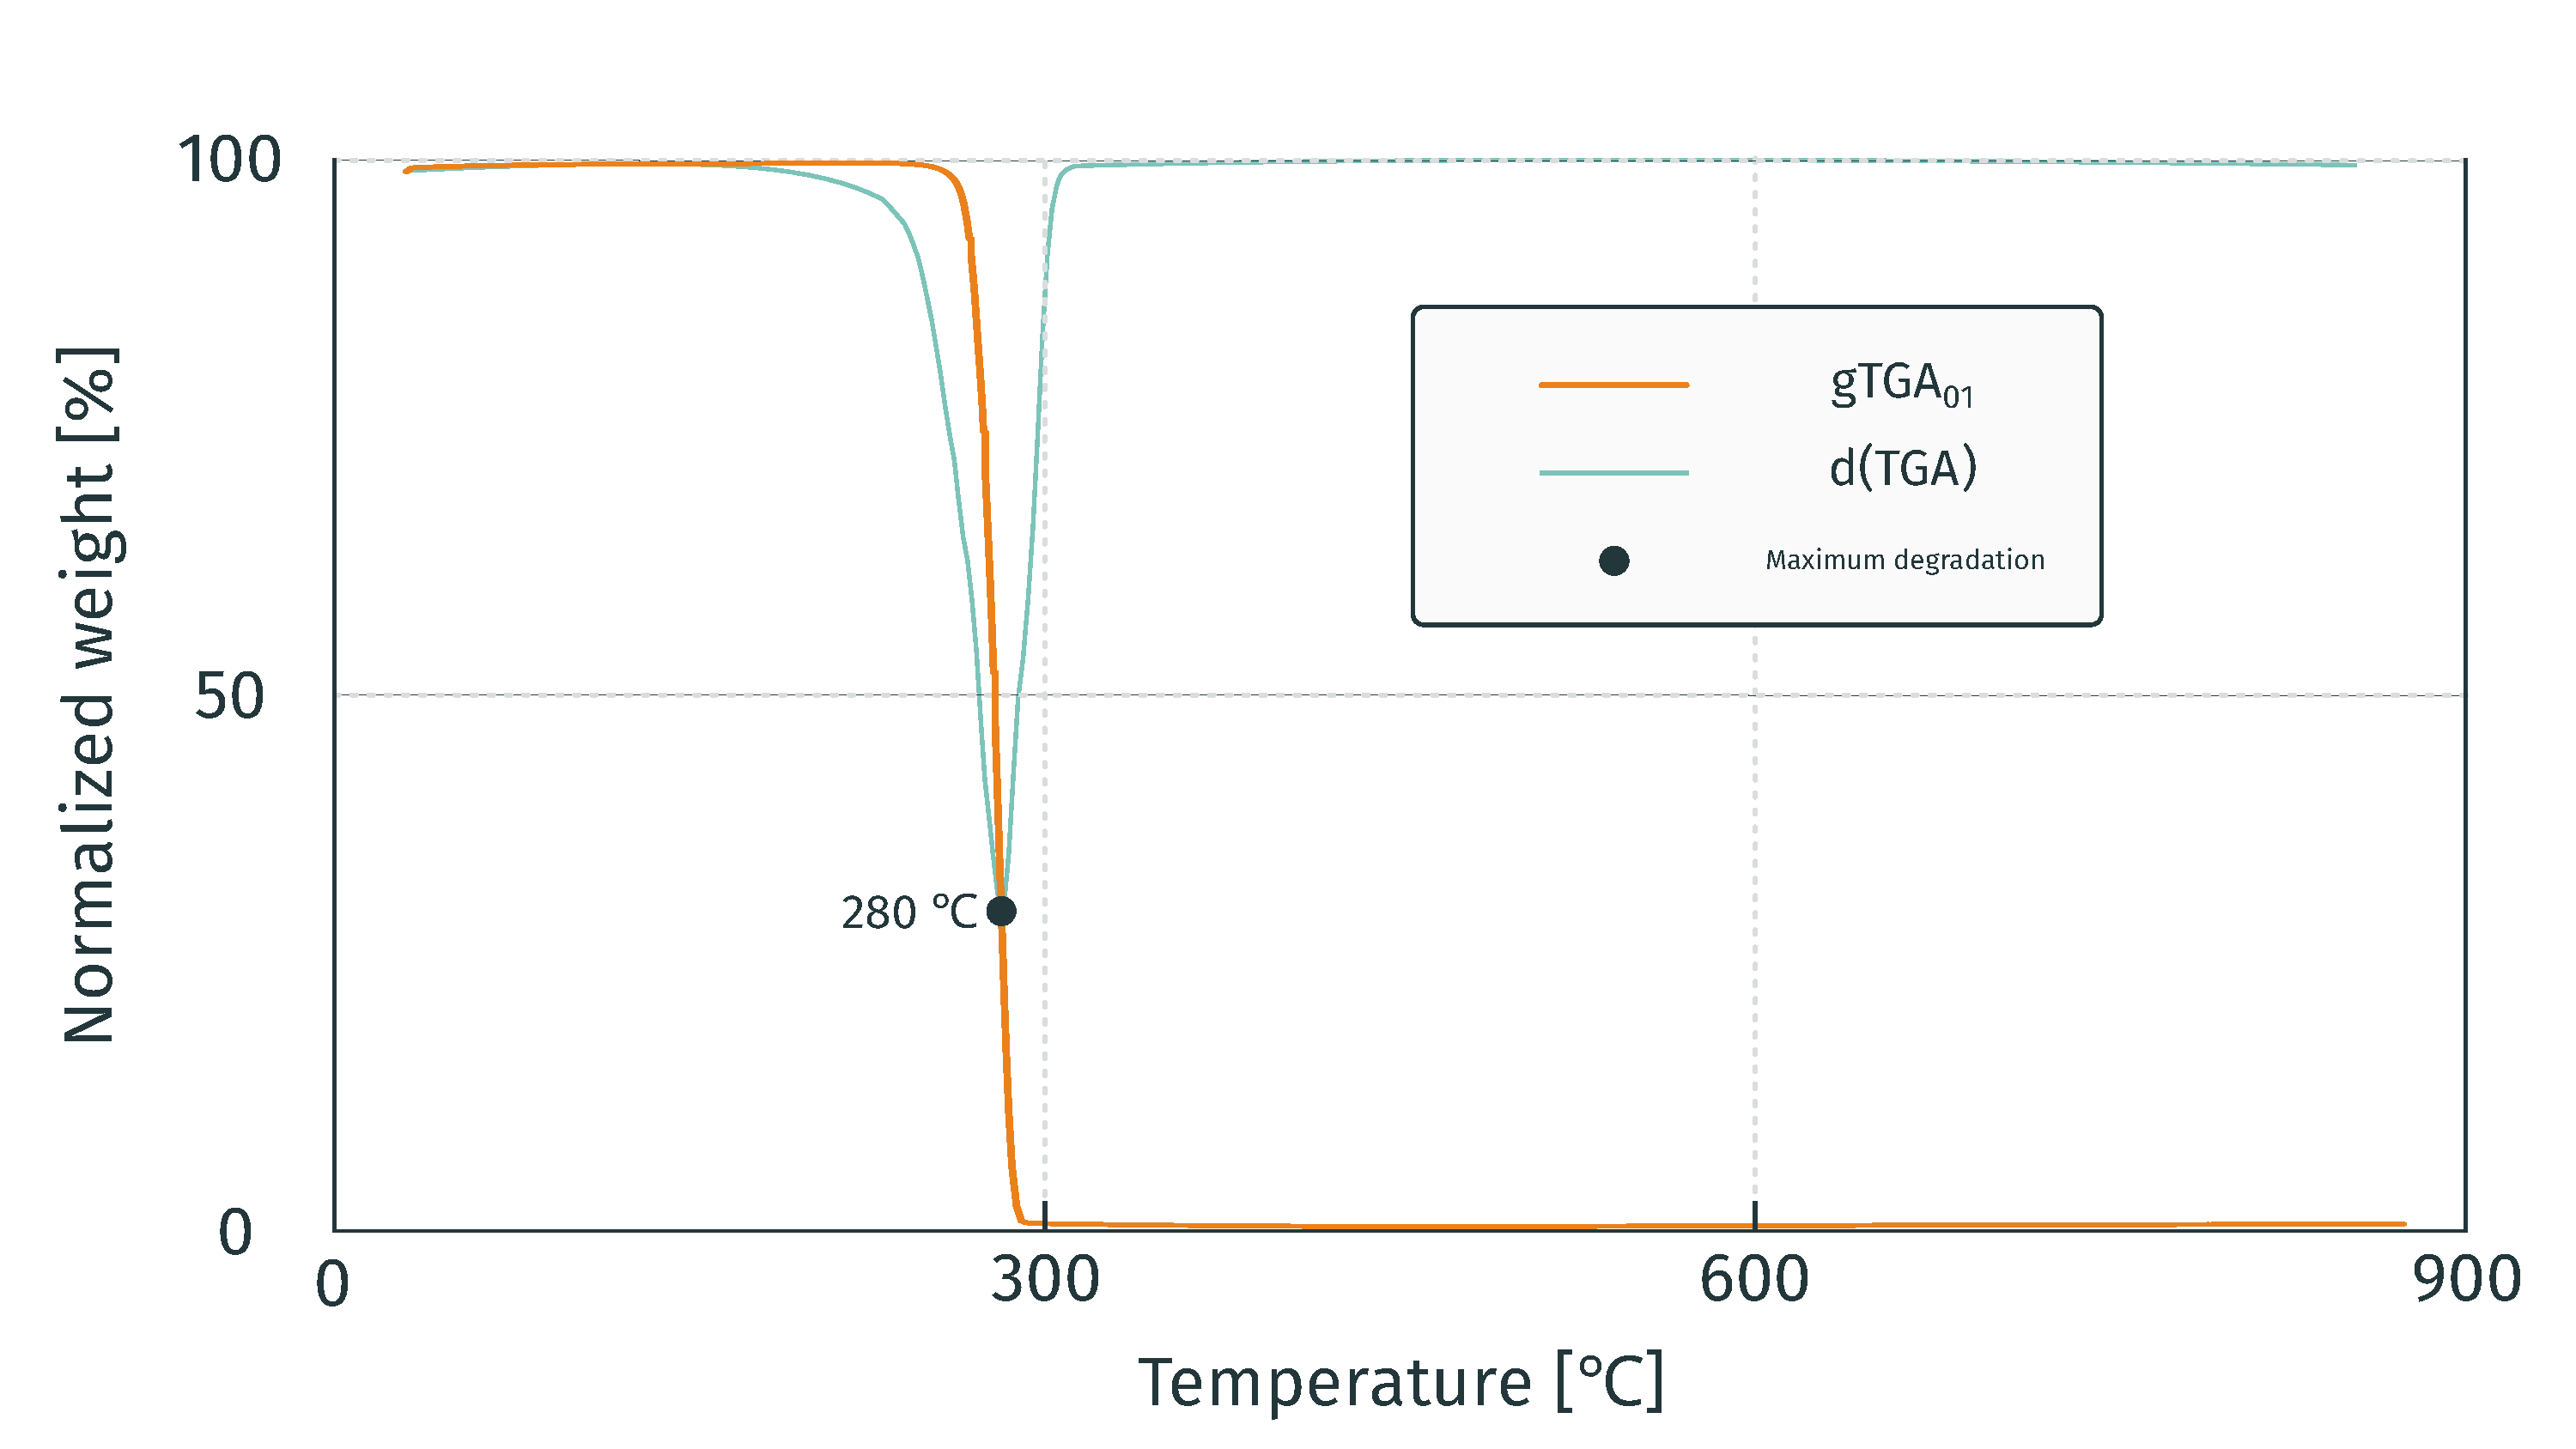
\includegraphics[width=0.8\textwidth]{Pictures/Vector/PDF/TGA/gTGA_derivative.pdf}
            \end{figure}
          }          

          \onslide*<6>{
            \begin{center}
              \alert{Come si comporta la polvere rispetto al pellet di materiale iniziale?}  
            \end{center}
          }

          \onslide*<7>{
            \begin{figure}[h]
              \centering
              \caption{TGA overlap}
              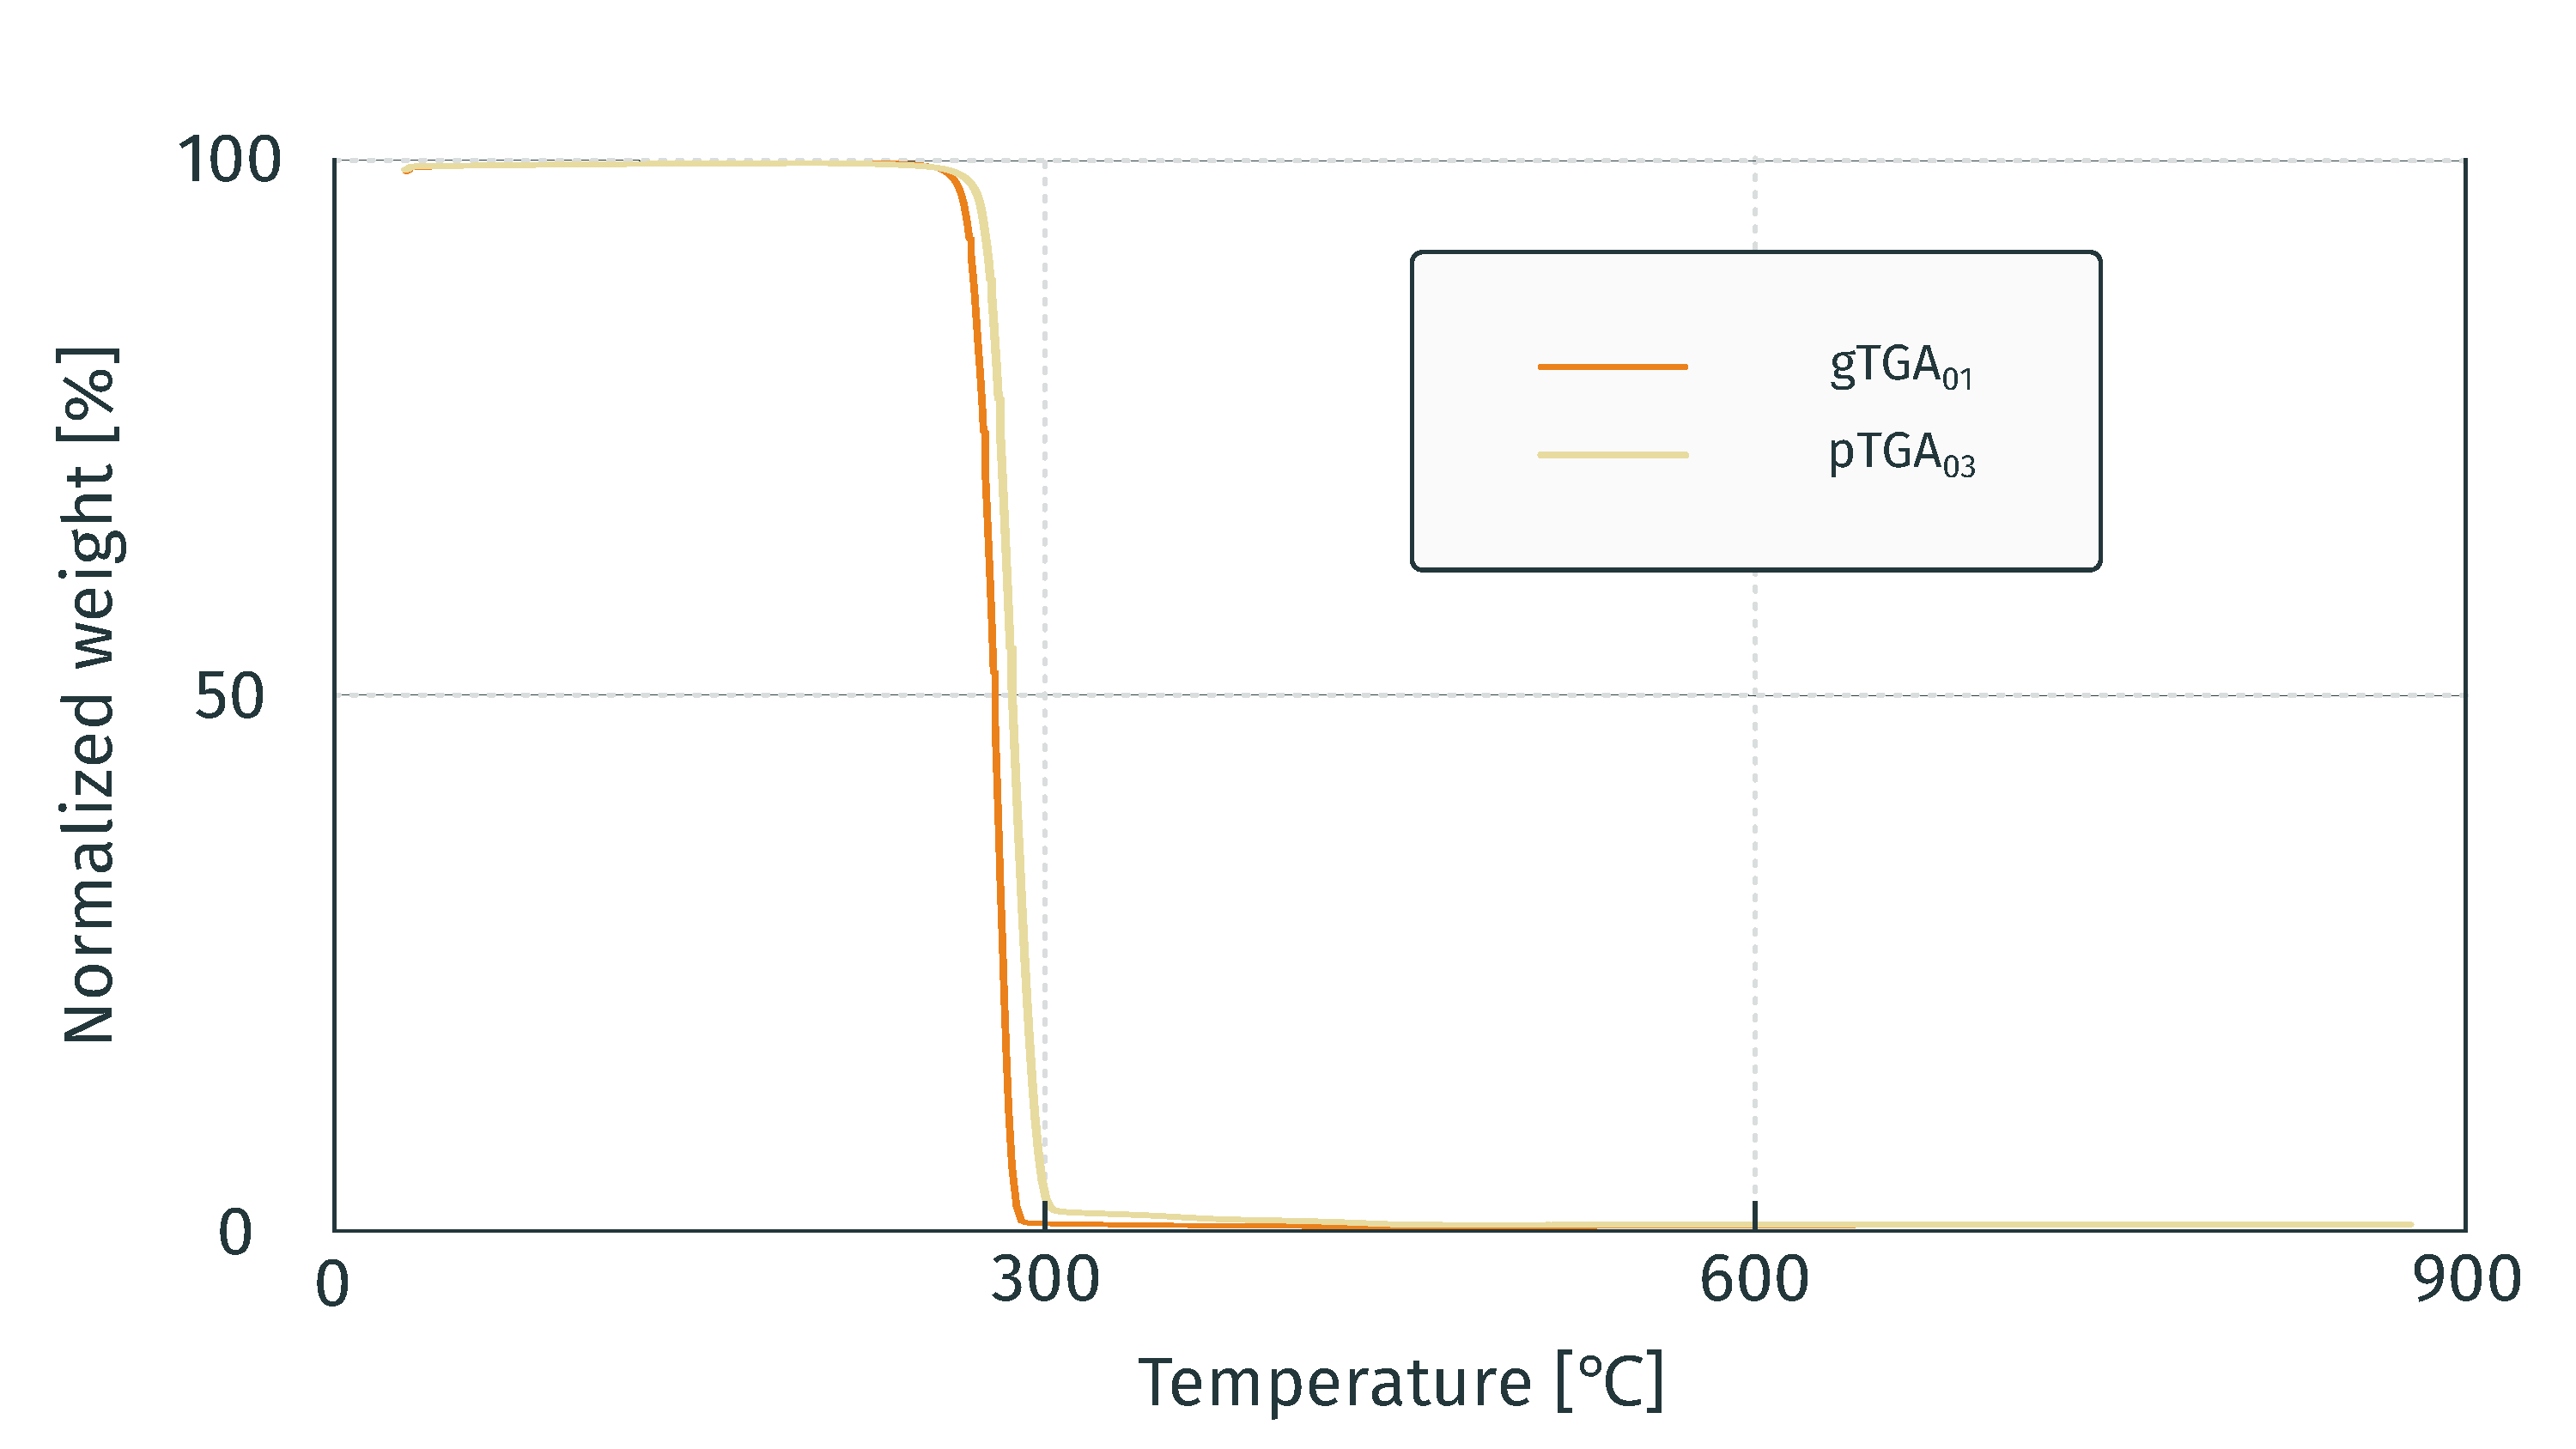
\includegraphics[width=0.8\textwidth]{Pictures/Vector/PDF/TGA/TGA_overlapped.pdf}
            \end{figure}
          }
          
        
        \end{frame}


\section{Stampa 3D}

  \begin{frame}
    \frametitle{Modellazione e Slicing}

    \onslide*<1>{
      \begin{center}
        \alert{Come si crea un oggetto da stampare in 3D?}
      \end{center}

    }

    \onslide*<2>{
      \begin{figure}[h]
        \centering
        \caption{Modellazione e triangolarizzazione della mesh}
        \includegraphics[width=0.75\textwidth]{Pictures/Vector/PDF/3dprinting_diagram-1.pdf}
        
      \end{figure}
    }

    \onslide*<3>{
      
      \begin{figure}
        \centering
        \caption{Slicing e generazione del G-CODE}
        \includegraphics[width=0.75\textwidth]{Pictures/Vector/PDF/3dprinting_diagram-2.pdf}
      \end{figure}
      
    }

    \onslide*<4>{
      \begin{figure}
        \centering
        \caption{Stampa}
        \includegraphics[width=0.75\textwidth]{Pictures/Vector/PDF/3dprinting_diagram-3.pdf}
      \end{figure}
    }

  
  \end{frame}

    \begin{frame}
      \frametitle{Modellazione e Slicing}

      \onslide*<1>{
        \begin{figure}[h]
          \centering
          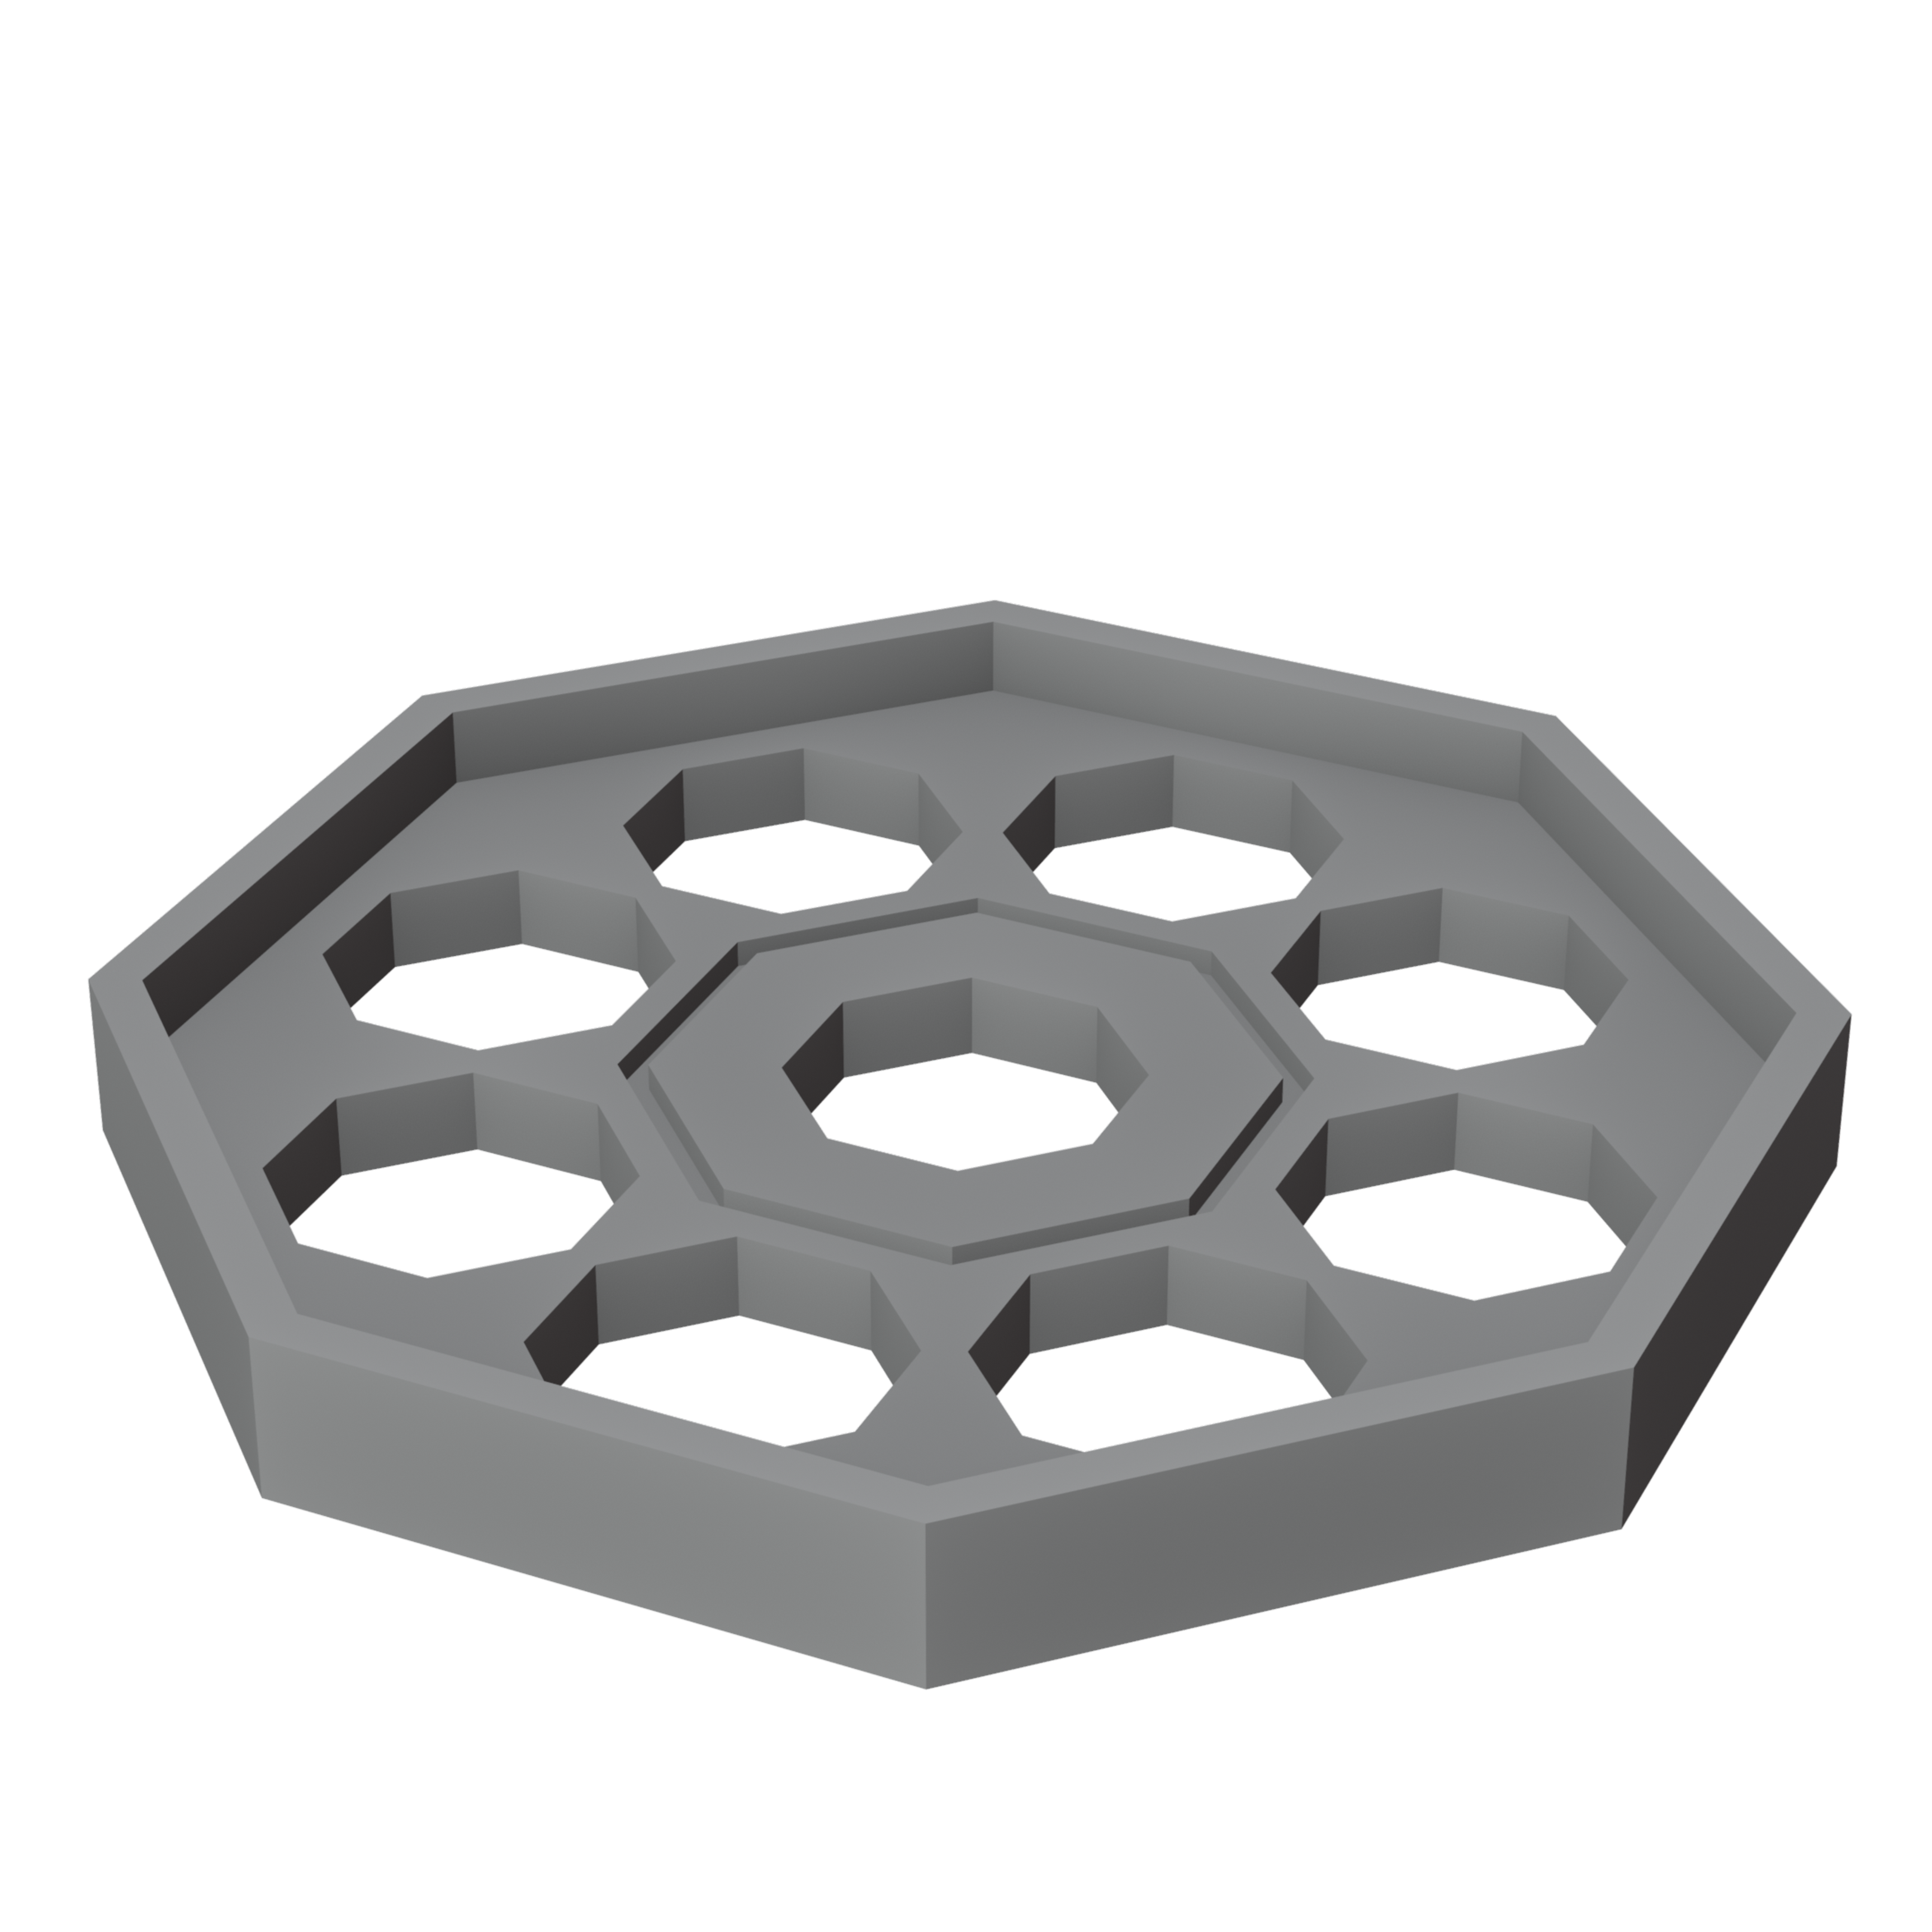
\includegraphics[width=0.5\textwidth]{Pictures/Vector/PDF/octagon_3D.pdf}
        \end{figure}
      }   
  
      \onslide*<2>{
        \begin{figure}[h]
          \centering
          \includegraphics[width=0.5\textwidth]{Pictures/Vector/PDF/octagon_halfrender.pdf}
        \end{figure}
      }
  
      \onslide*<3>{
        \begin{figure}[h]
          \centering
          \includegraphics[width=0.5\textwidth]{Pictures/Vector/PDF/octagon_render.pdf}
        \end{figure}
      }
    
    
      
    
    \end{frame}

  \begin{frame}
    \frametitle{Setup}

    \onslide*<1>{

      \begin{figure}[h]
        \centering
        \caption{Sharebot SnowWhite$^2$}
        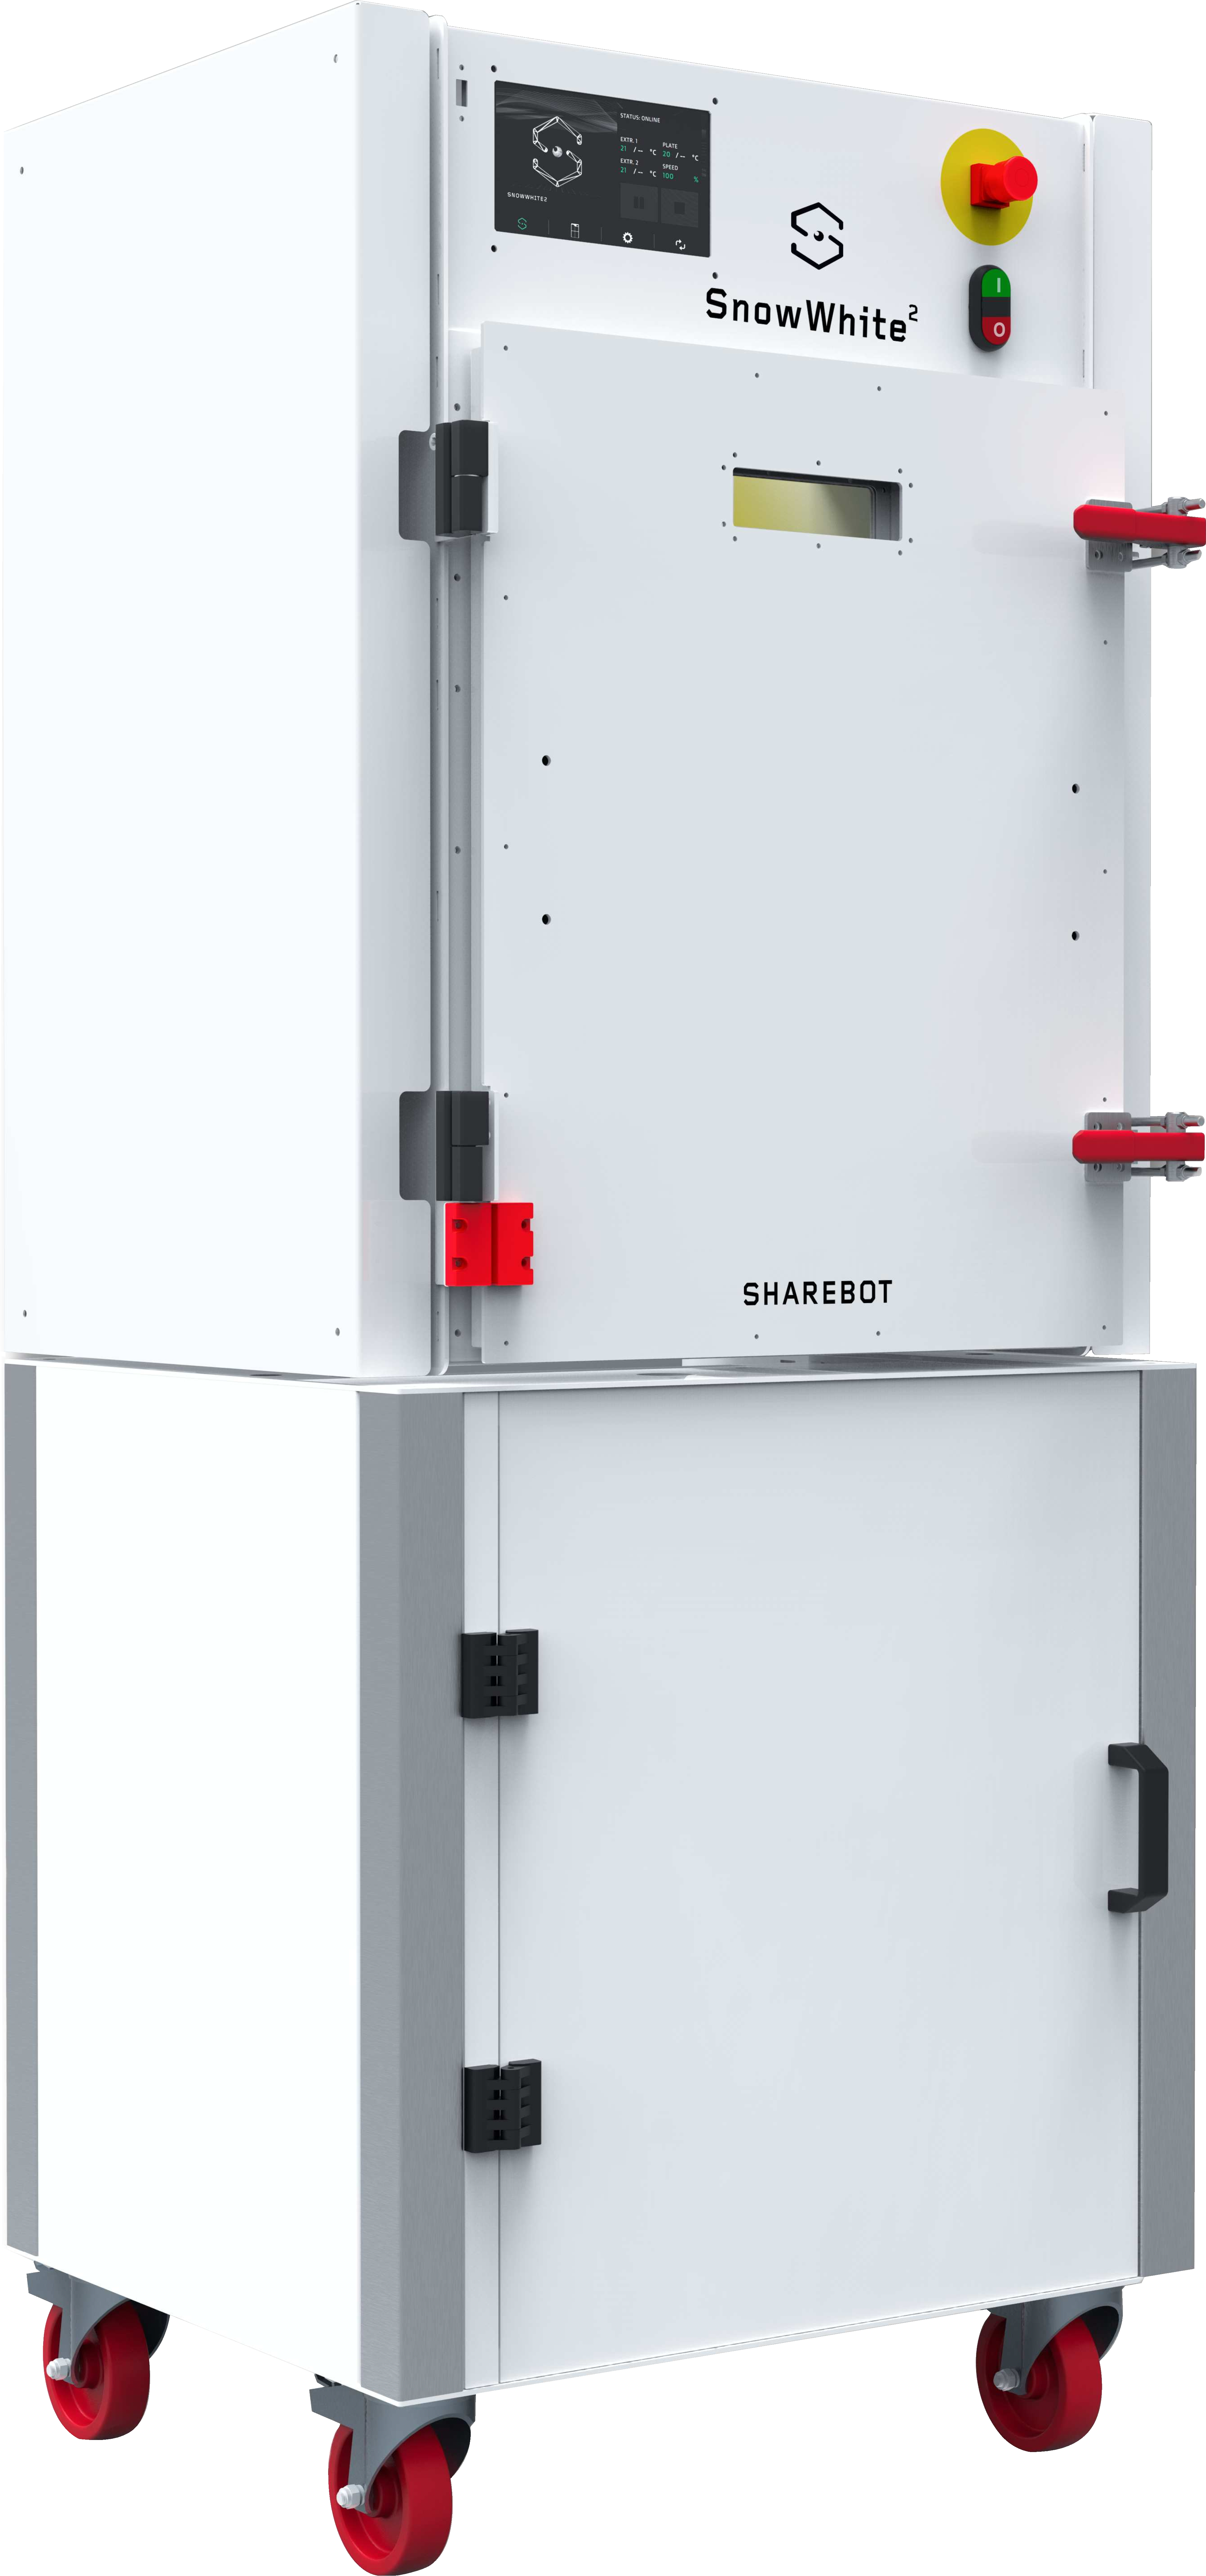
\includegraphics[width=0.2\textwidth]{Pictures/Vector/PDF/sharebot_snowhite2.pdf}
      \end{figure}
    }

    \onslide*<2>{
        
        \begin{figure}[h]
          \centering
          \caption{Touch UI}
          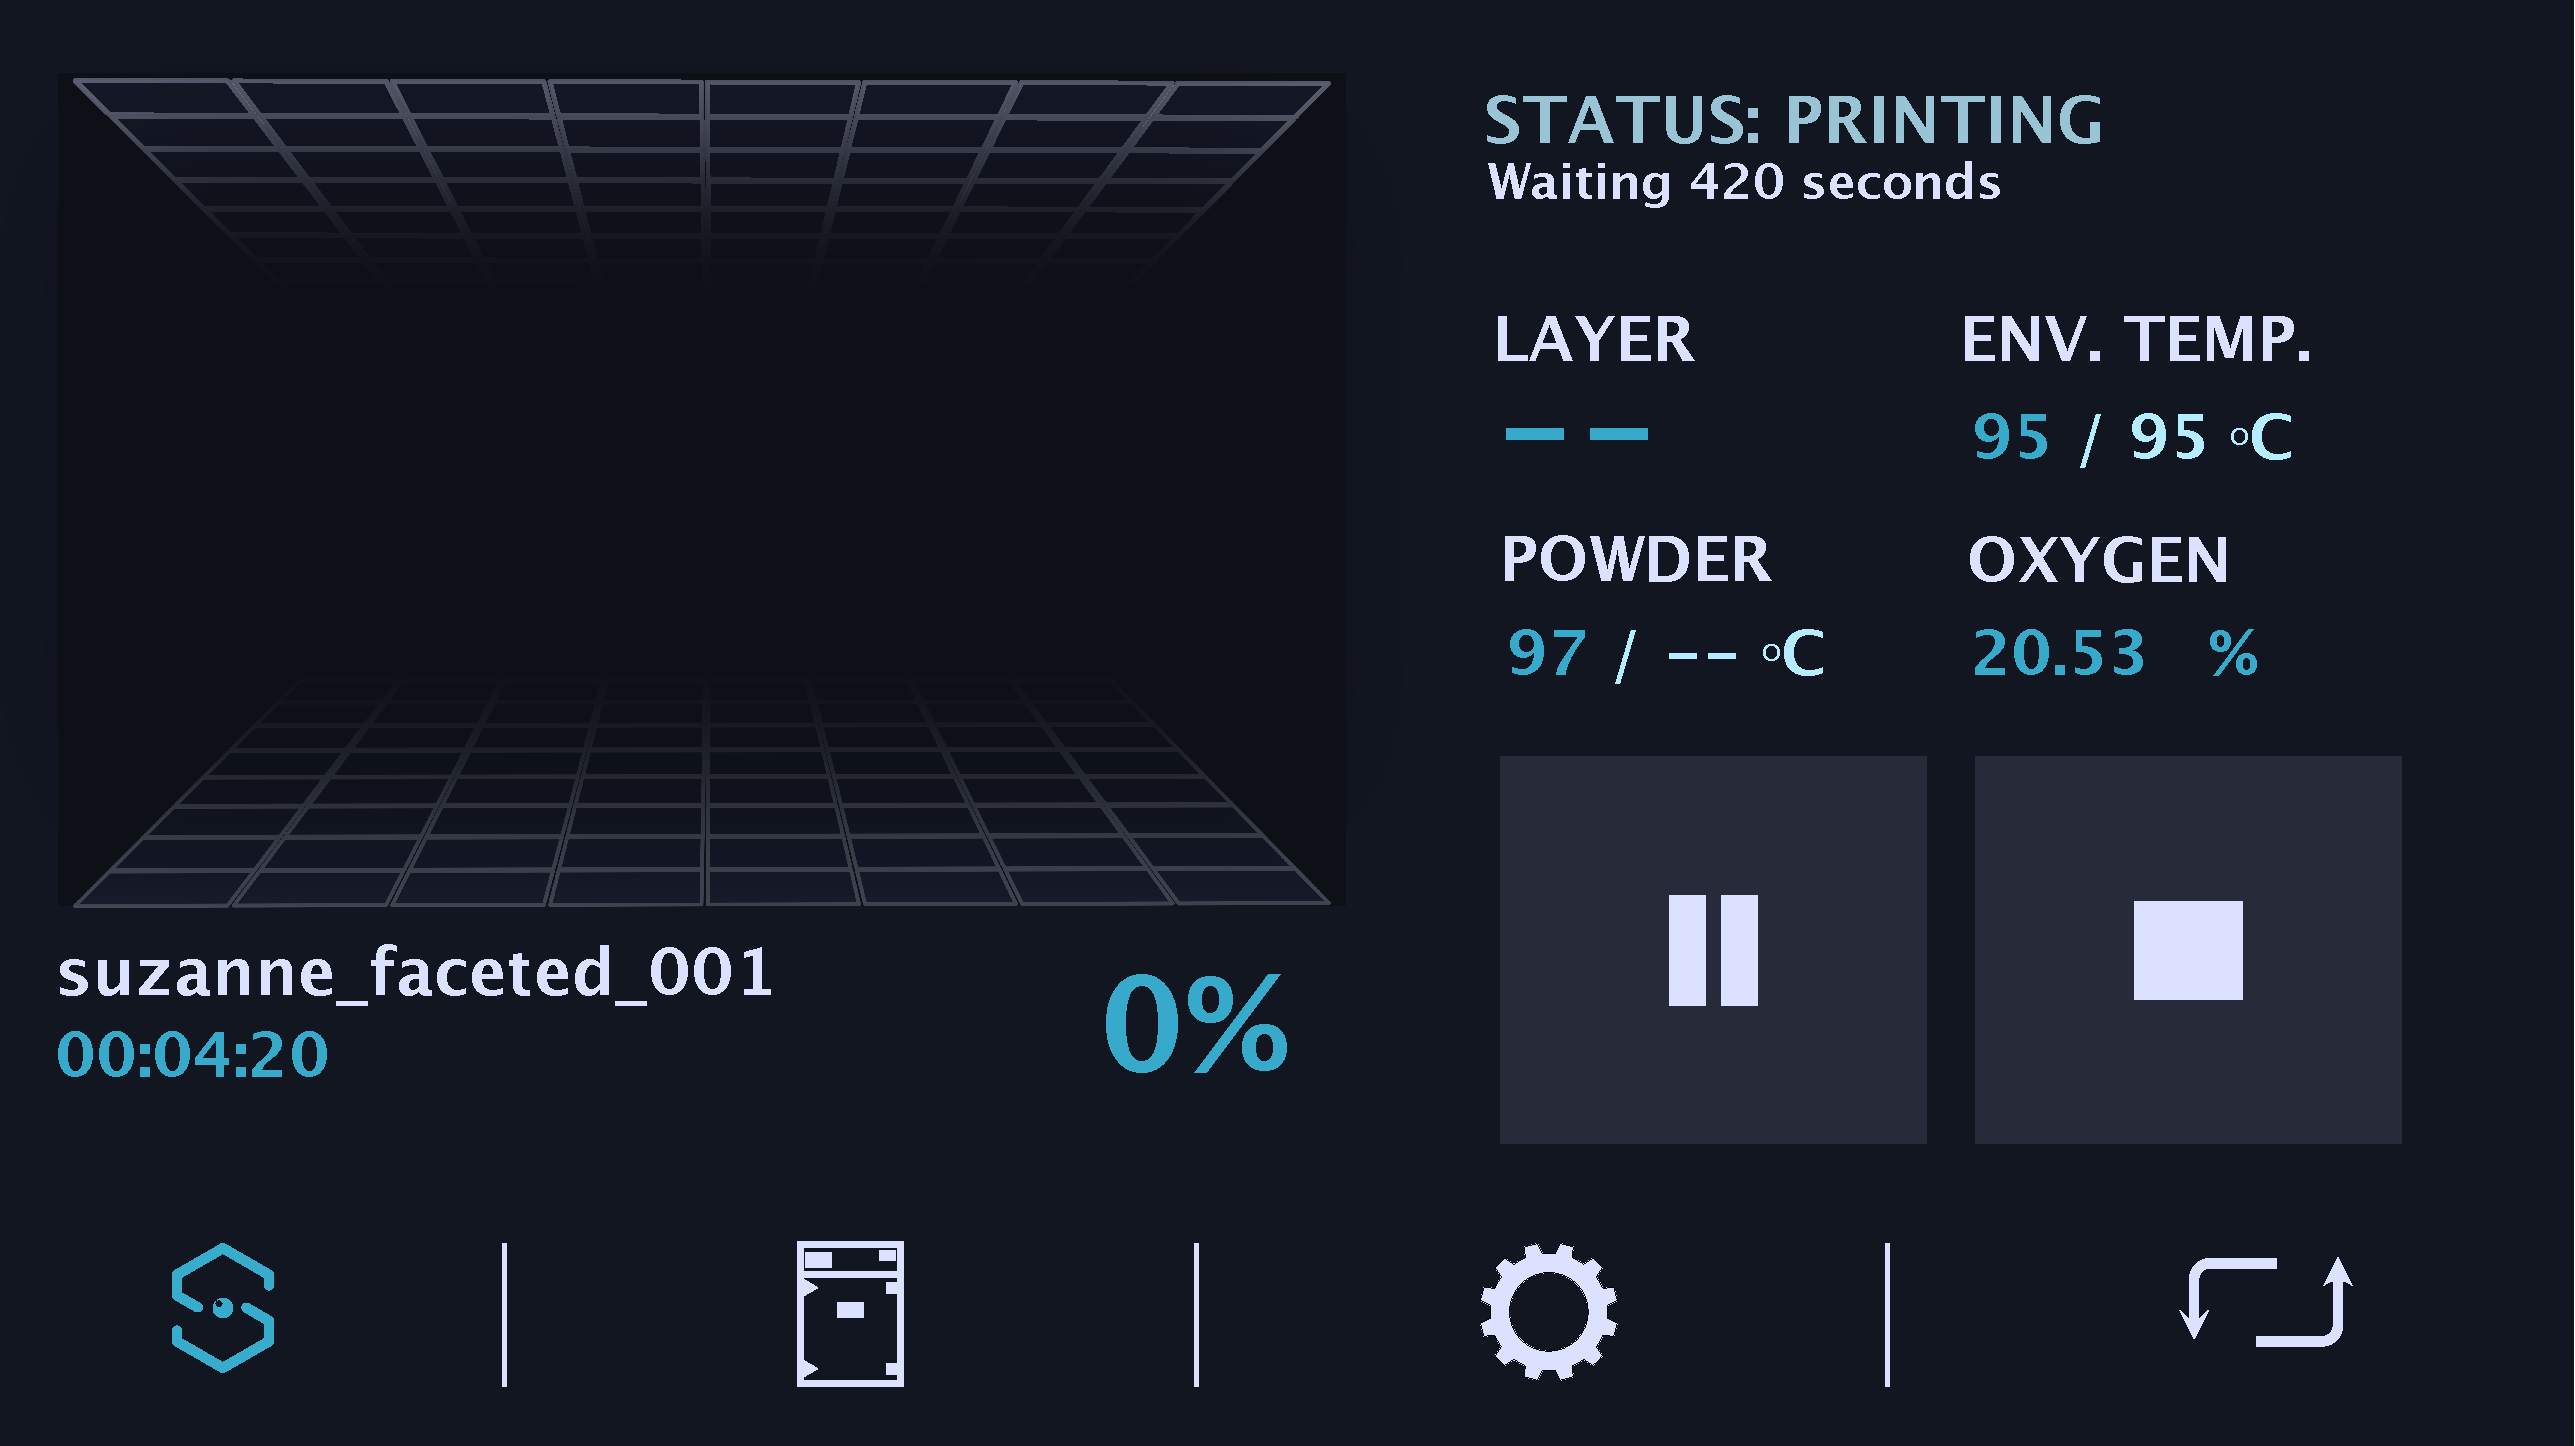
\includegraphics[width=0.8\textwidth]{Pictures/Vector/PDF/Sharebot_GUI.pdf}
        \end{figure}
    }

    \onslide*<3-6>{
      \begin{center}
        \alert<3>{Quali sono i parametri di stampa fondamentali?}
      \end{center}
    }

    \begin{itemize}
      \item <4-6> \textbf{Temperatura ambientale}
      \item <5-6> \textbf{Temperatura del letto di polvere}
      \item <6> \textbf{Potenza del laser}
    \end{itemize}

    \onslide*<4>{Ottimale tra 85 e 95 $ ^{\circ}C$, a seconda della geometria stampata}
    \onslide*<5>{Deve rimanere all'interno della finestra di sinterizzazione}
    \onslide*<6>{Ottimale tra 25 \% e il 35 \% della potenza massima (14 W), a seconda della geometria stampata}



  \end{frame}

  \begin{frame}
    \frametitle{Risultati}

      \onslide*<1>{
        \begin{center}
          \alert{Quali sono i risultati ottenuti?}
        \end{center}
      }

    \onslide*<2>{

      \begin{figure}[h]
        \centering
        \caption{Campioni DMA}
        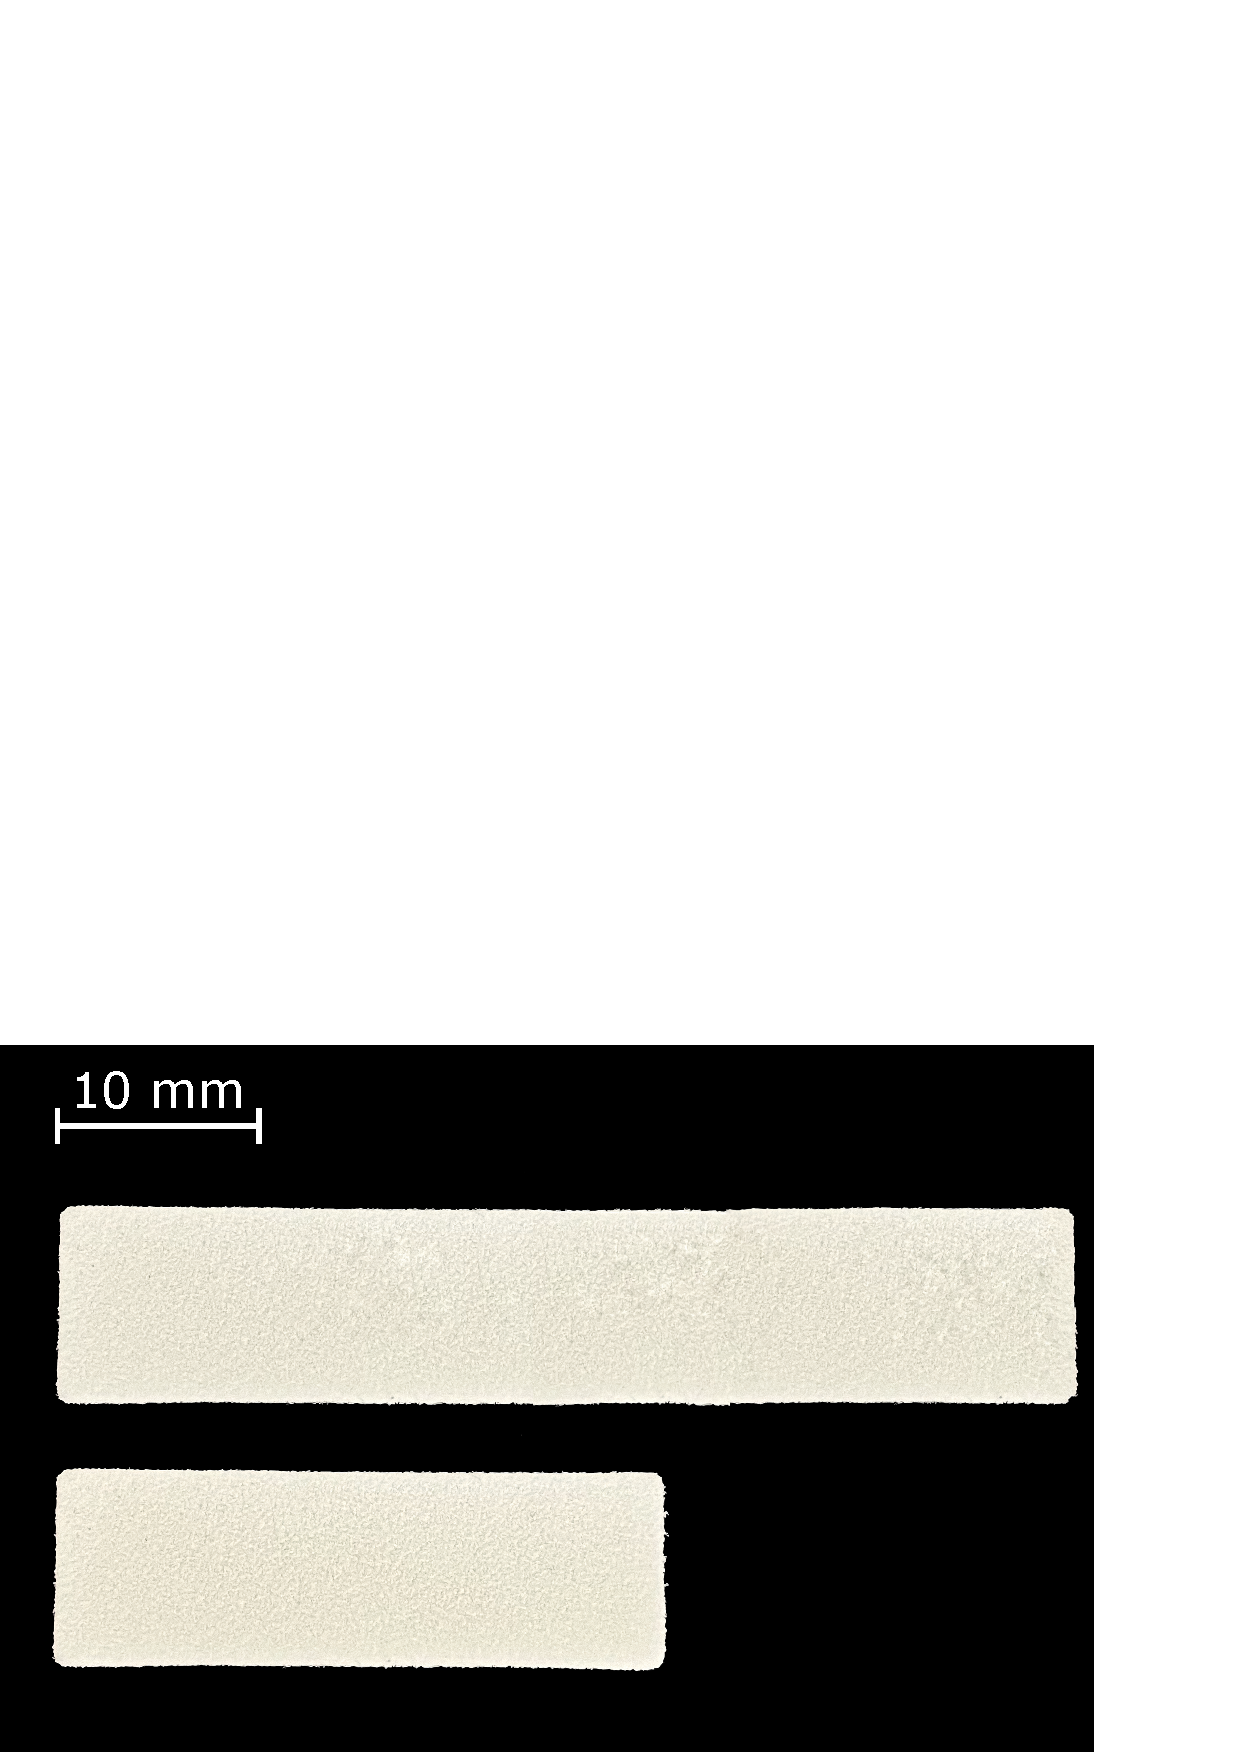
\includegraphics[width=0.6\textwidth]{Pictures/Vector/PDF/Printed_parts/DMA_samples.pdf}
      \end{figure}
    }

    \onslide*<3>{

    \begin{figure}[h]
      \centering
      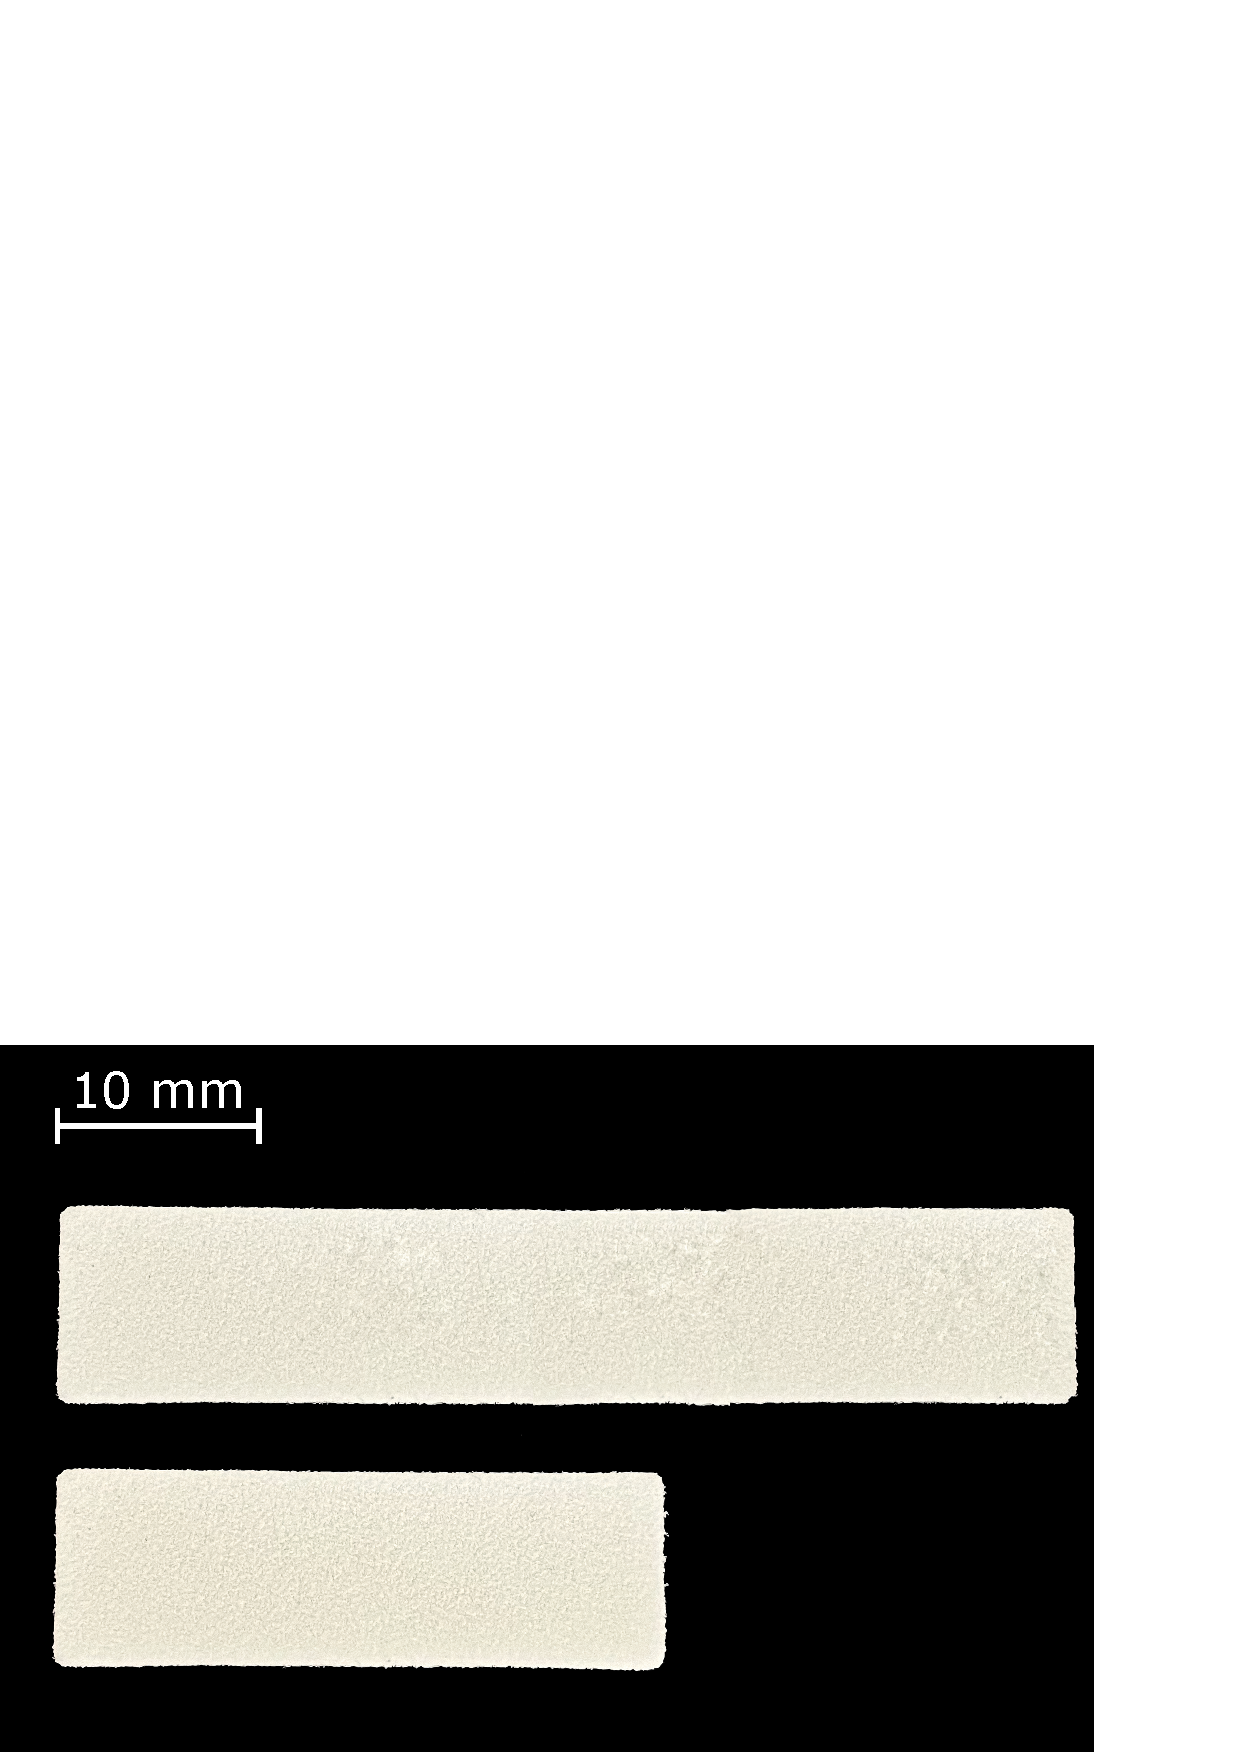
\includegraphics[width=0.4\textwidth]{Pictures/Vector/PDF/Printed_parts/DMA_samples.pdf}
    \end{figure}

      Campioni prismatici, 15 e 10 layer rispettivamente (1.5 e 1.0 mm), stampati con potenza del 25 \% (3.5 W) a 90 $ ^{\circ}C$.
    }

    \onslide*<4>{

      \begin{figure}[h]
        \centering
        \caption{Esagono con pattern intricato}
        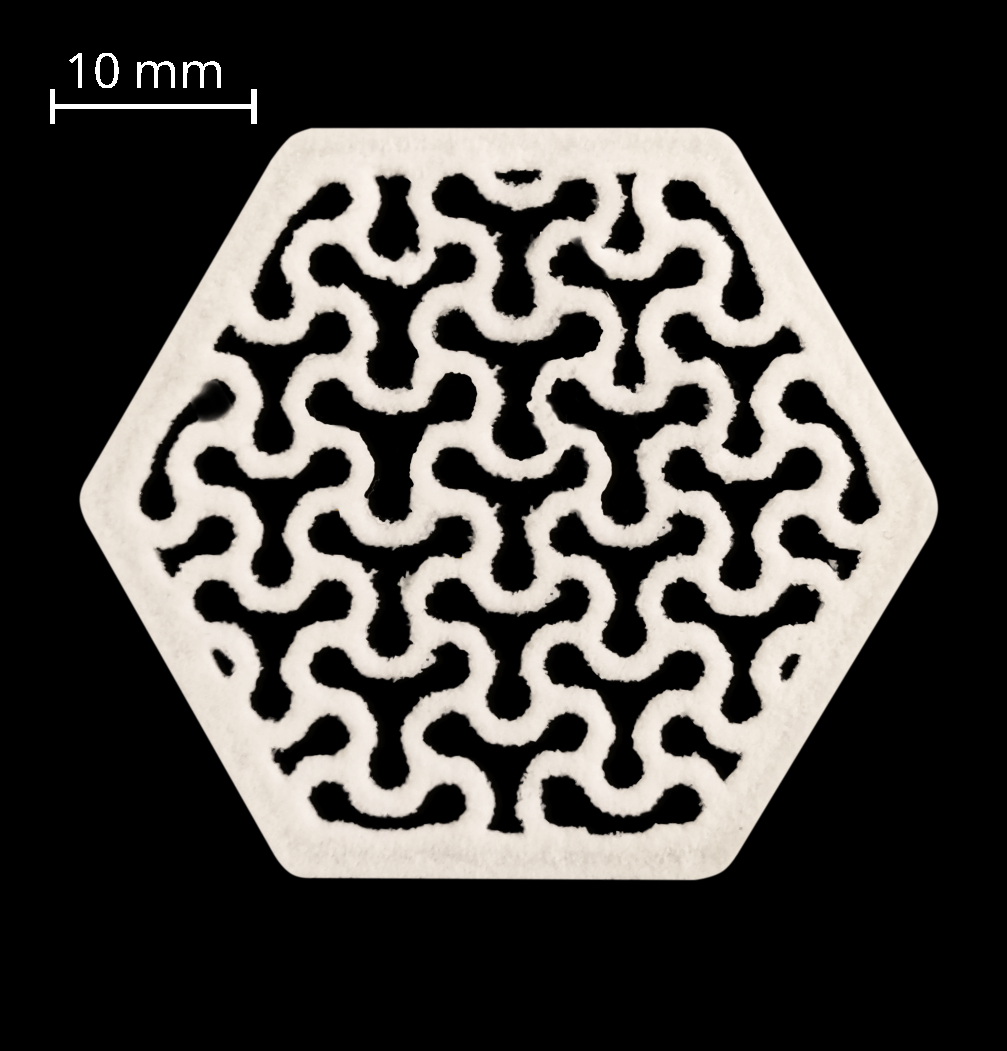
\includegraphics[width=0.4\textwidth]{Pictures/Vector/PDF/Printed_parts/organic_pattern.pdf}
      \end{figure}
    }

    \onslide*<5>{

      \begin{figure}[h]
        \centering
        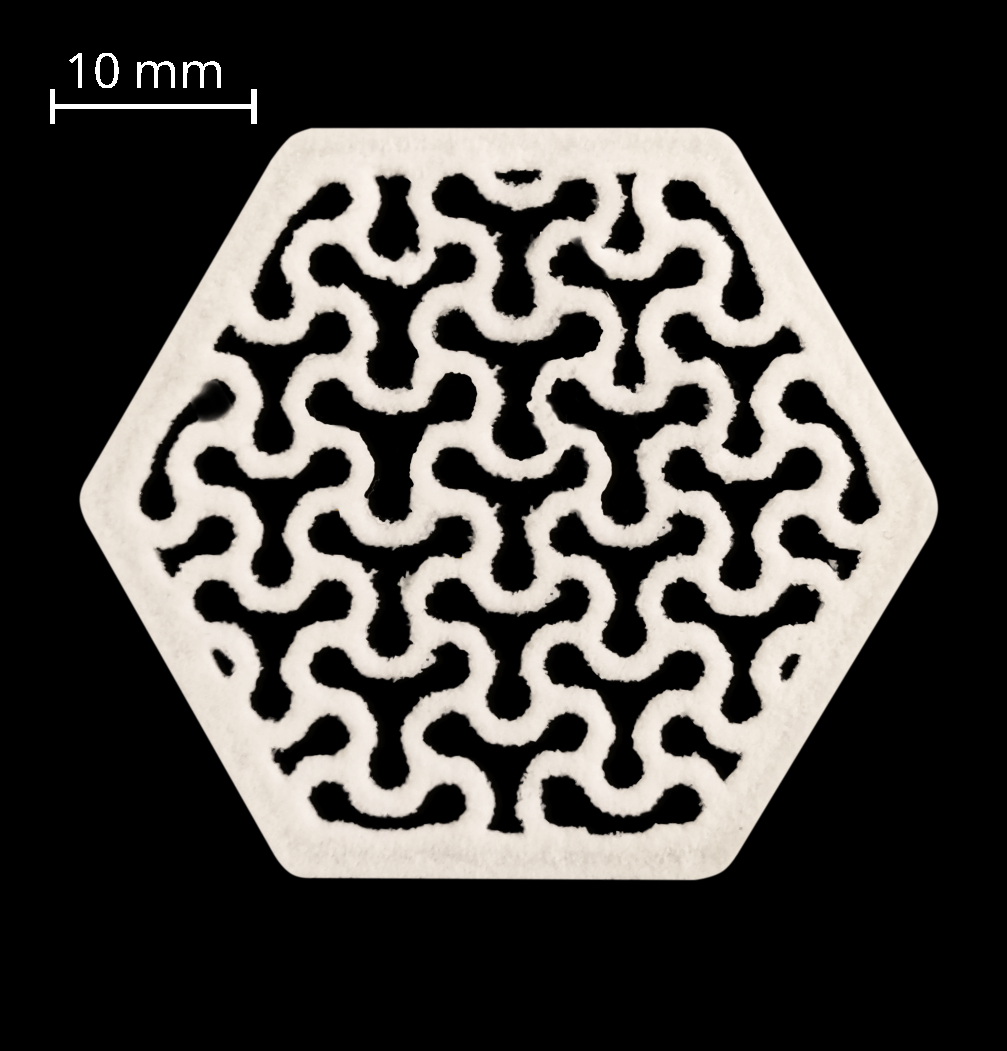
\includegraphics[width=0.25\textwidth]{Pictures/Vector/PDF/Printed_parts/organic_pattern.pdf}
      \end{figure}

      Campione con trama sottile, 15 layer (1.5 mm), stampato con potenza del 35 \% (4.9 W) a 87 $ ^{\circ}C$.
    }

    \onslide*<6>{

      \begin{figure}[h]
        \centering
        \caption{Imbarcazione con pareti sottili e curve}
        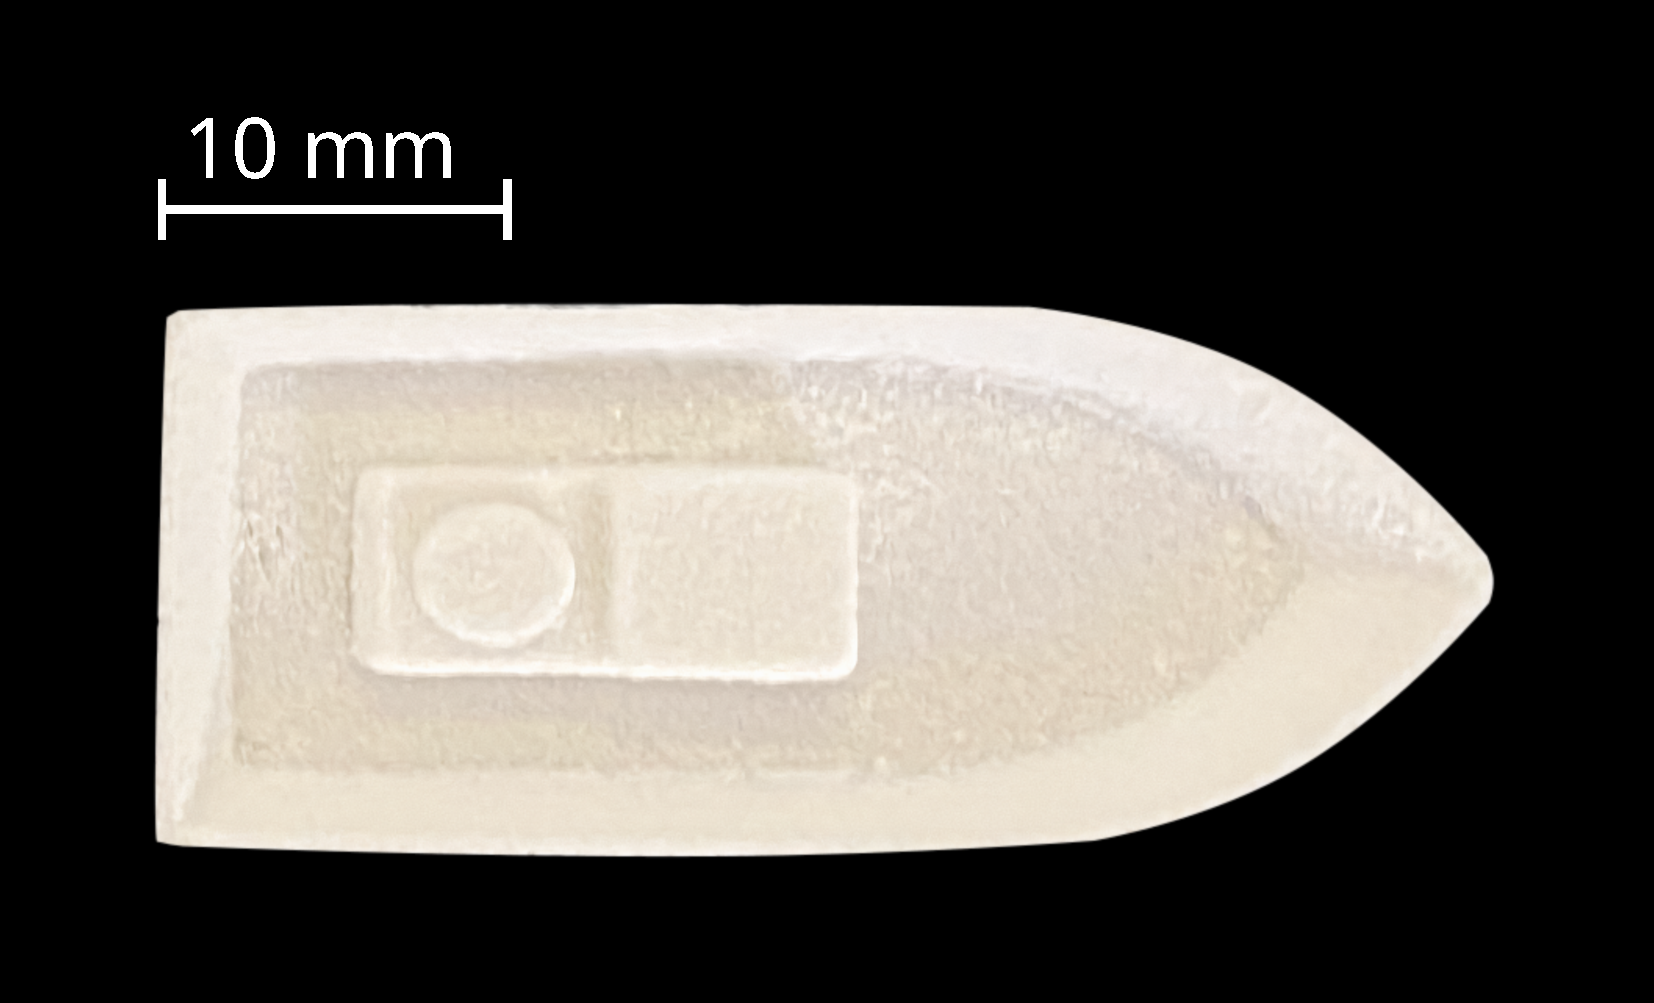
\includegraphics[width=0.6\textwidth]{Pictures/Vector/PDF/Printed_parts/boat.pdf}
      \end{figure}
    }

    \onslide*<7>{

      \begin{figure}[h]
        \centering
        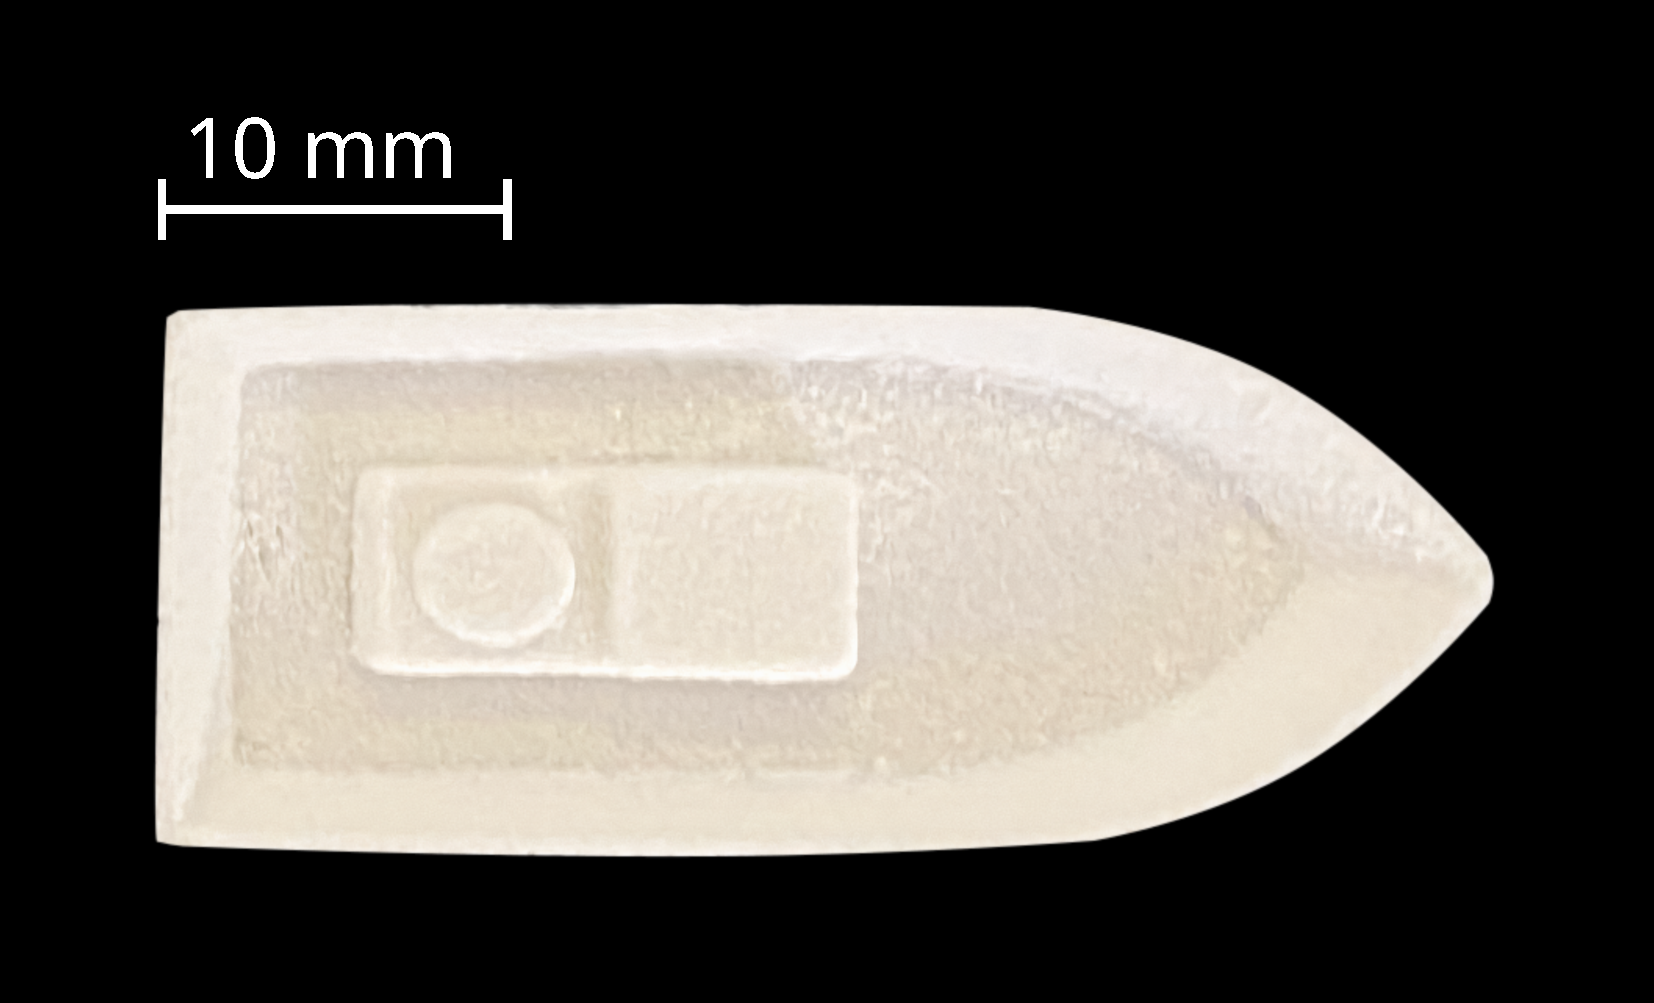
\includegraphics[width=0.4\textwidth]{Pictures/Vector/PDF/Printed_parts/boat.pdf}
      \end{figure}

      Campione con pareti sottili e curve, 50 layer (5 mm), stampato con potenza del 30 \% (4.20 W) a 90 $ ^{\circ}C$.
    }

    \onslide*<8>{

      \begin{figure}[h]
        \centering
        \caption{Ottagono con bordo sottile e array di fori ottagonali}
        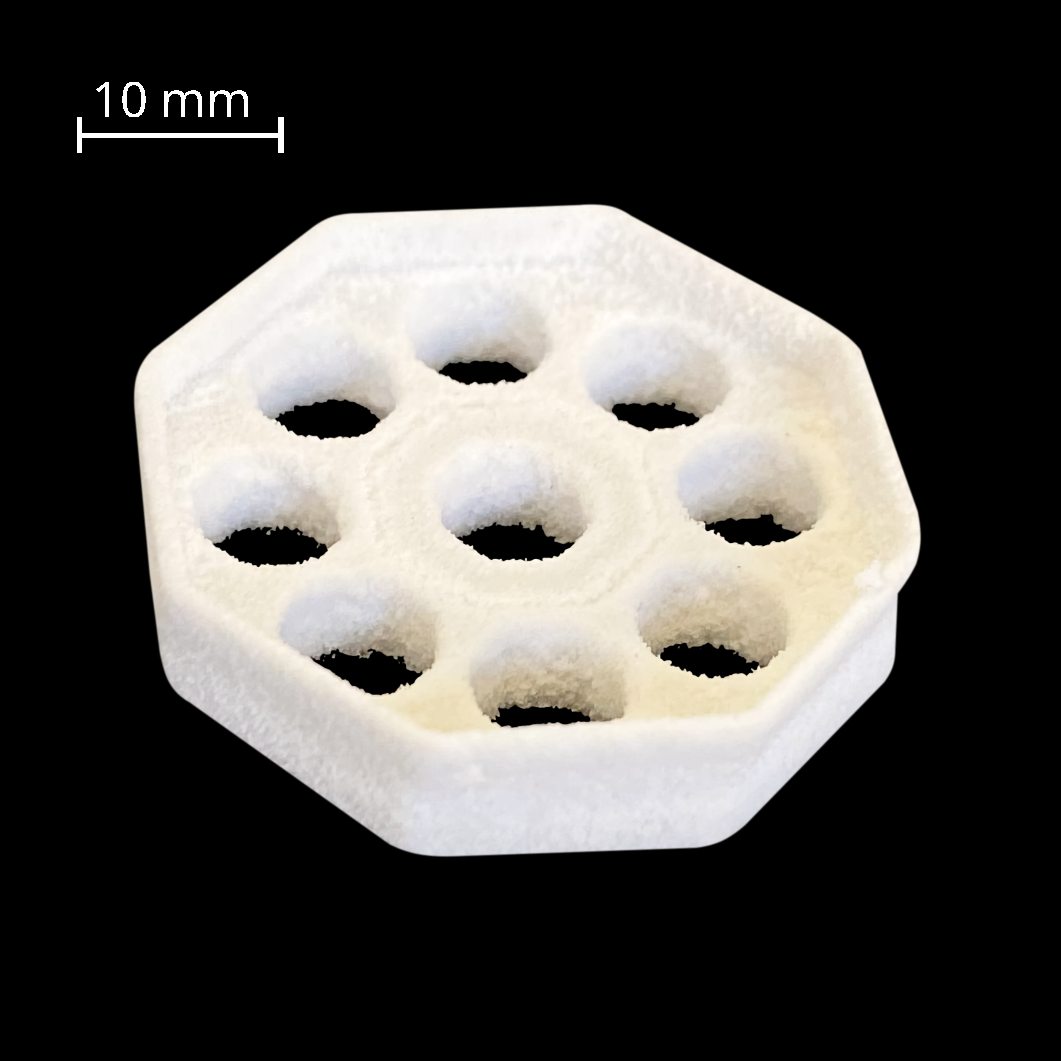
\includegraphics[width=0.4\textwidth]{Pictures/Vector/PDF/Printed_parts/octagon_holes.pdf}
      \end{figure}
    }

    \onslide*<9>{

      \begin{figure}[h]
        \centering
        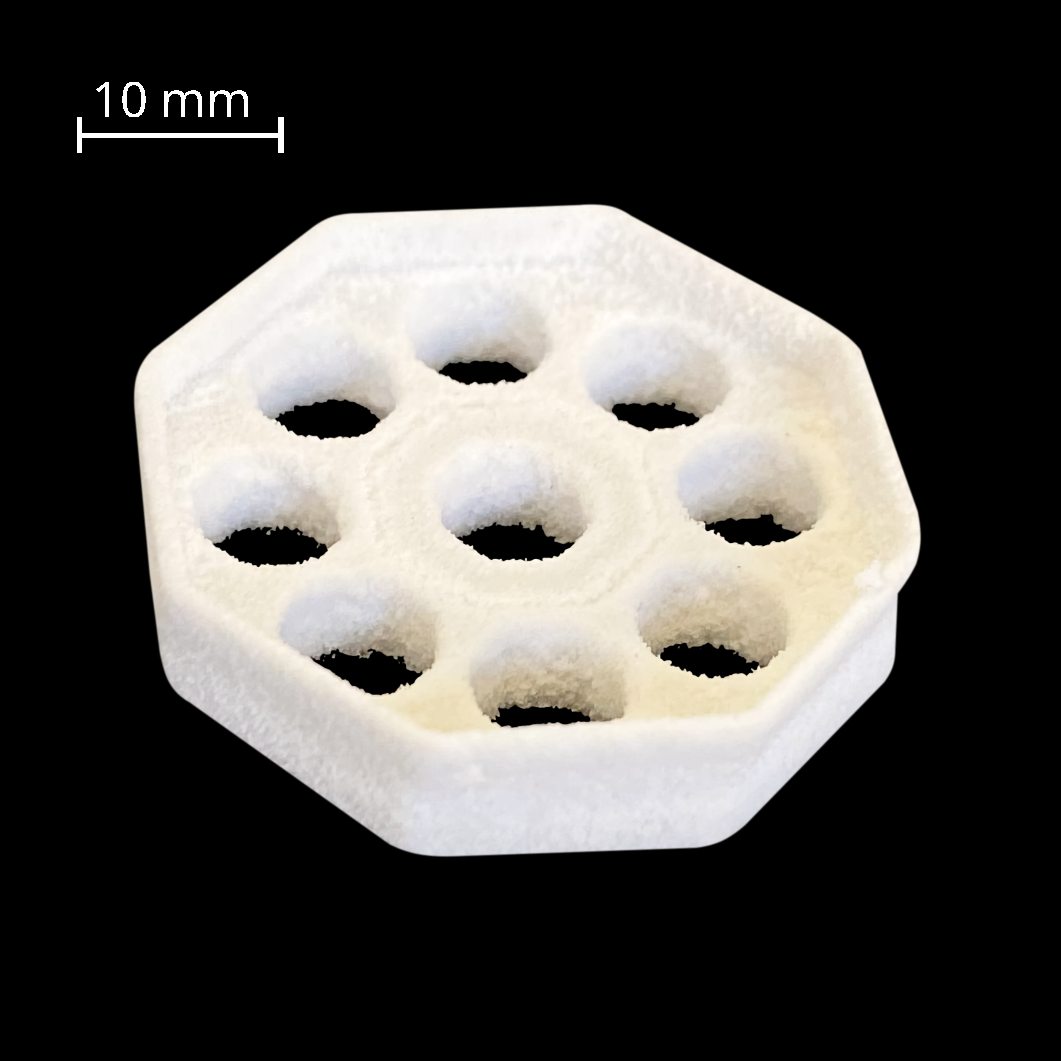
\includegraphics[width=0.25\textwidth]{Pictures/Vector/PDF/Printed_parts/octagon_holes.pdf}
      \end{figure}

      Campione con bordo sottile e array di fori ottagonali, 55 layer (5.5 mm), stampato con potenza del 35 \% (4.9 W) a 95 $ ^{\circ}C$.
    }
  
    
  
  \end{frame}

  \begin{frame}
    \frametitle{Analisi Meccanica Dinamica}

      \onslide*<1>{
        \begin{center}
          \alert{Analisi Meccanica Dinamica}
        \end{center}
      }

      \onslide*<2>{L'\textbf{analisi meccanica dinamica} (DMA) è un'analisi termica utilizzata per lo studio delle proprietà viscoelastiche dei materiali. \\ 
      La prova è stata svolta applicando un carico sinusoidale di 1 N a 1 Hz su un campione di prova, al crescere della temperatura.}
      \onslide*<3-7>{
        \begin{center}
          Quali caratteristiche fondamentali sono state analizzate?
        \end{center}

      }

      \begin{itemize}
        \item <4-7> \textbf{Modulo di conservazione $E'$}
        \item <5-7> \textbf{Modulo di perdita $E''$}
        \item <6-7> \textbf{Fattore di smorzamento $tan \delta = \frac{E''}{E'}$}
        \item <7>  \textbf{Temperatura di transizione vetrosa $T_g$}

      \end{itemize}

      \onslide*<4>{Il modulo di conservazione è indice del comportamento elastico del materiale.}
      \onslide*<5>{Il modulo di perdita è indice della dissipazione di energia sotto forma di calore.}
      \onslide*<6>{Il fattore di smorzamento è il rapporto tra i due moduli.}
      \onslide*<7>{La temperatura di transizione vetrosa è deducibile dal massimo della $tan \delta$, con maggiore precisione rispetto ad una DSC.}

 
  
    
  
  \end{frame}

    \begin{frame}
      \frametitle{Analisi Meccanica Dinamica}

      \onslide*<1>{

        \begin{figure}[h]
          \centering
          \caption{Prova DMA per un campione di PHBH stampato in SLS}
          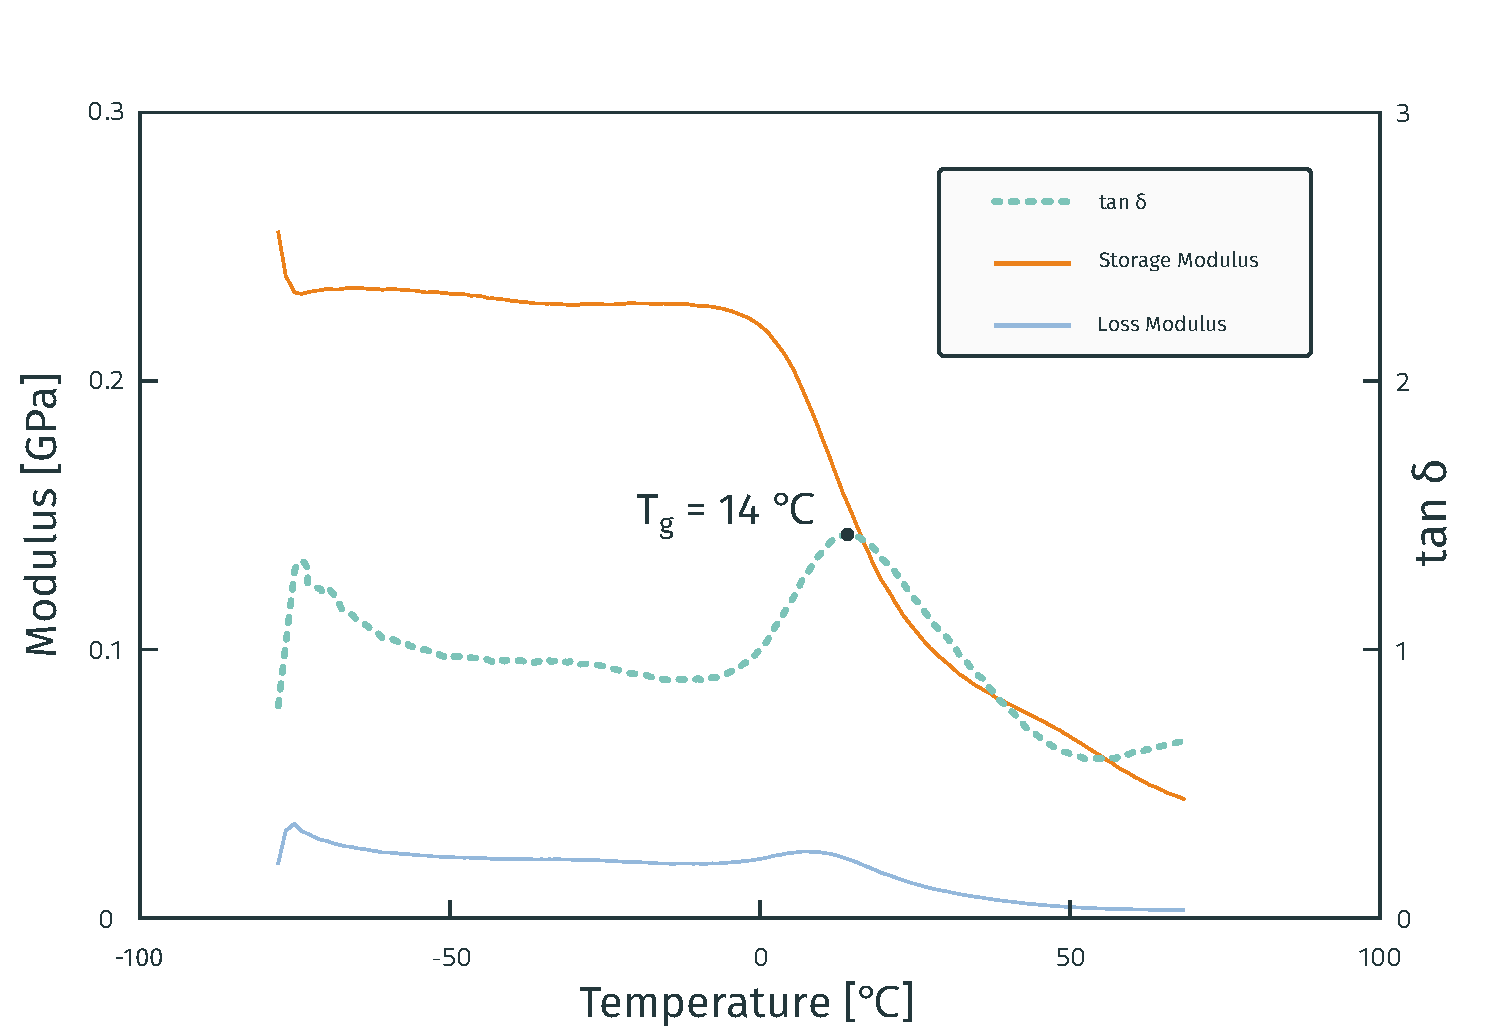
\includegraphics[width=0.6\textwidth]{Pictures/Vector/PDF/DMA.pdf}
        \end{figure}

      }

      \onslide*<2>{

        \begin{figure}[h]
          \centering
          \caption{Moduli}
          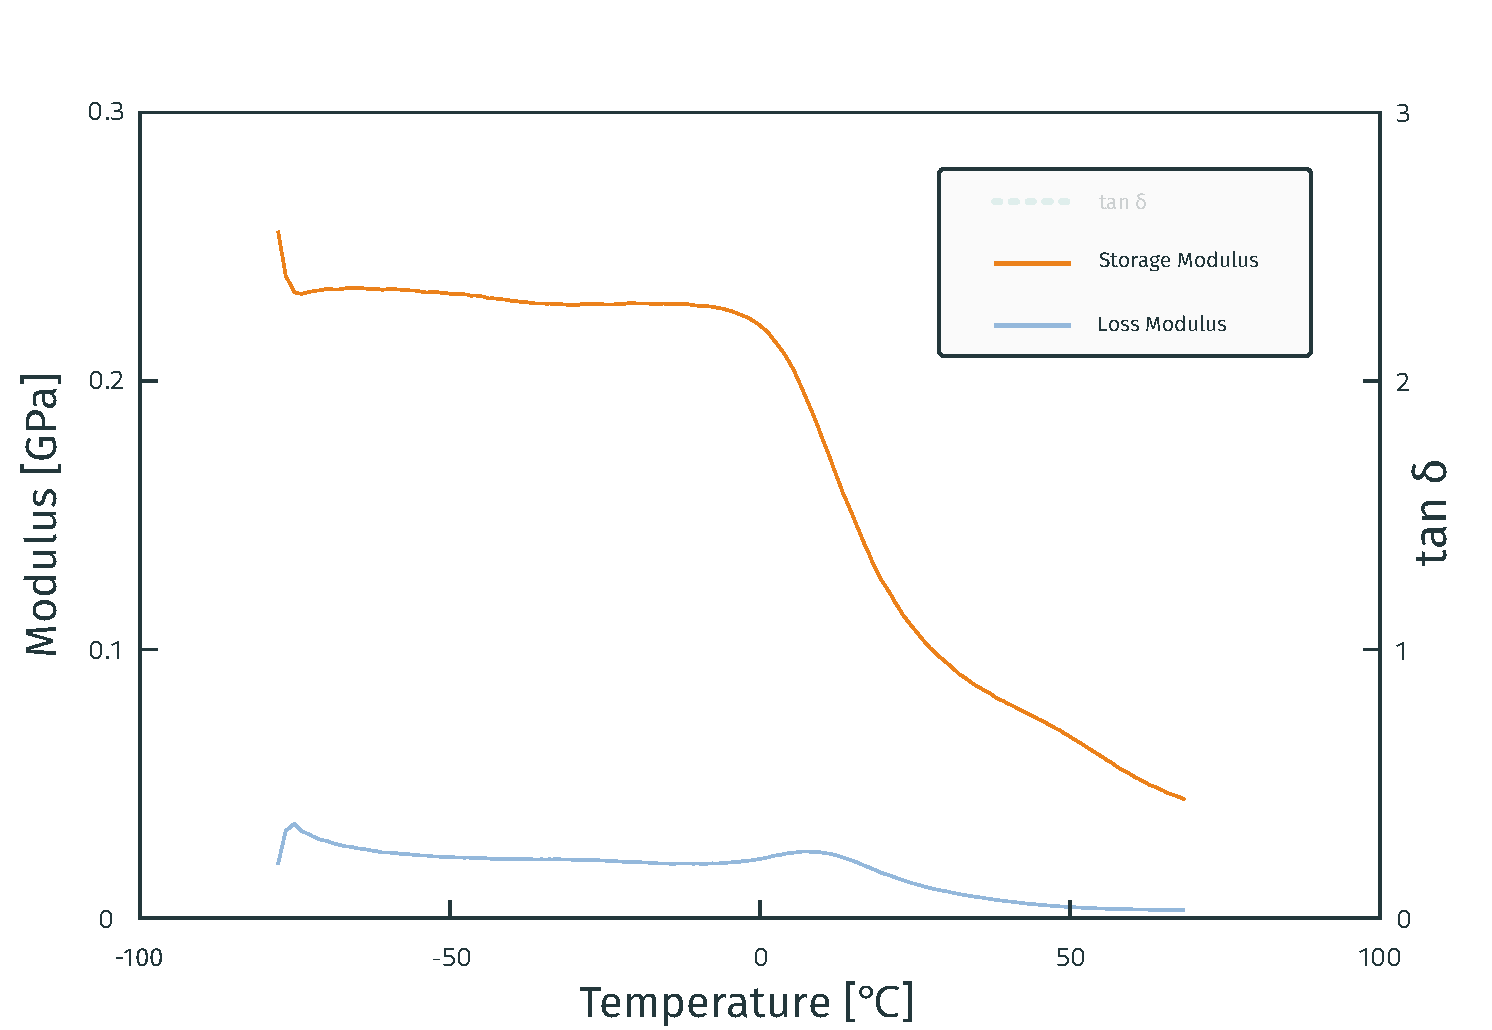
\includegraphics[width=0.6\textwidth]{Pictures/Vector/PDF/DMA-1.pdf}
        \end{figure}

      }

      \onslide*<3>{

        \begin{figure}[h]
          \centering
          \caption{Temperatura di transizione vetrosa}
          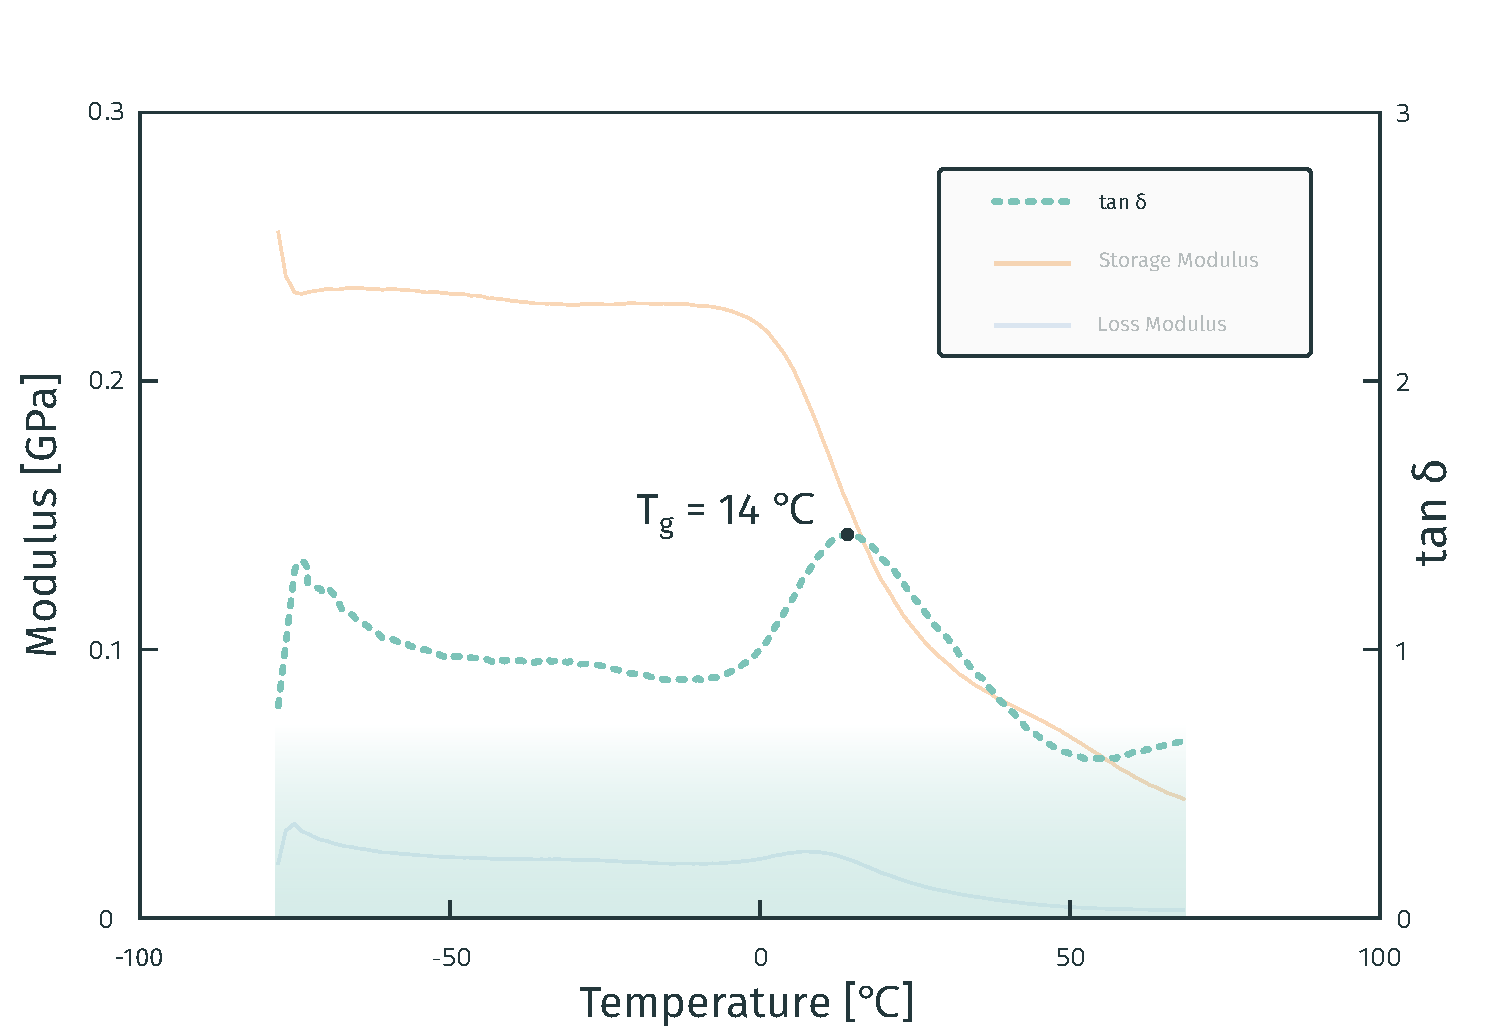
\includegraphics[width=0.6\textwidth]{Pictures/Vector/PDF/DMA-2.pdf}
        \end{figure}

      }
    
    
    \end{frame}

  \begin{frame}
    \frametitle{Stabilità termica}

    \onslide*<1>{
      \begin{center}
        \alert{Come si comporta termicamente il PHBH una volta stampato?}
      \end{center}
    }

    \onslide*<2>{A conferma dell'ottima stabilità termica del PHBH, è stata effettuata un'altra \textbf{analisi termogravimetrica}}

    \onslide*<3>{

      \begin{figure}[h]
        \centering
        \includegraphics[width=0.9\textwidth]{Pictures/Vector/PDF/TGA/TGA_final-1.pdf}
      \end{figure}

    }

    \onslide*<4>{

      \begin{figure}[h]
        \centering
        \includegraphics[width=0.9\textwidth]{Pictures/Vector/PDF/TGA/TGA_final-2.pdf}
      \end{figure}

    } 

    \onslide*<5>{

      \begin{figure}[h]
        \centering
        \includegraphics[width=0.9\textwidth]{Pictures/Vector/PDF/TGA/TGA_final-3.pdf}
      \end{figure}

    }
  
    
  
  \end{frame}


\section{Conclusioni}

  \begin{frame}
    \frametitle{Innovazione}
  
      \onslide*<1-5>{
        \begin{center}
          \alert<1>{Risultati ottenuti ben oltre le aspettative ed estremamente innovativi}
        \end{center}
      }

      \begin{itemize}
        \item <2-5> Produzione di polvere di PHBH ad \textbf{alto rendimento} ed SLS ready
        \item <3-5> Riproducibilità e \textbf{scalabilità} della produzione di polvere
        \item <4-5> Stampa \textbf{SLS} di elevata risoluzione e con ottima \textbf{stabilità termica}
        \item <5>   Enorme \textbf{potenziale applicativo} 
        
        \end{itemize}
  
  \end{frame}

    \begin{frame}
      \frametitle{Pubblicazione}

      \onslide*<1-2>{
        \begin{center}
          Il lavoro è parte di una pubblicazione, al momento in peer review, per la rivista \textbf{Materials Today Sustainability}:
        \end{center}
      }

      \onslide*<2>{
        \begin{center}  
          \textit{Novel 3D Printable Bio-based and Biodegradable Poly(3-hydroxybutyrate-co-3-
          hydroxyhexanoate) Microspheres for Selective Laser Sintering Applications} \\ 

          
          A. Giubilini, G. Colucci, G. De Trane, F. Lupone, C. Badini, P. Minetola, F. Bondioli, M. Messori
        \end{center}
      
      }
    
      
    
    \end{frame}

    %{\setbeamercolor{}{fg=Foreground, bg=Background}
      \begin{frame}[standout]
        Grazie per l'attenzione
      \end{frame}
    %}



    \begin{frame}[allowframebreaks]{Bibliografia}
    
        \nocite{Padovano_SLS_Review}
        \nocite{SLS_3dprinting_biomedical_polymers}
        \nocite{Messori_Bondioli_PHAs}
        \nocite{Solutions_plastic_pollution}
        \nocite{AM_design_review}
        \nocite{DechetMaximilianA2020OtDo}
        \printbibliography

    
    \end{frame}





\end{document}